\documentclass{article}
\usepackage[preprint,nonatbib]{neurips_2026} \usepackage[numbers]{natbib}


\usepackage[utf8]{inputenc}
\usepackage[T1]{fontenc}
\usepackage{hyperref}
\usepackage{url}
\usepackage{booktabs}
\usepackage{amsfonts}
\usepackage{amsmath}
\usepackage{amssymb}
\usepackage{nicefrac}
\usepackage{microtype}
\usepackage{xcolor}
\usepackage{graphicx}
\usepackage{subcaption}
\usepackage{algorithm}
\usepackage{algorithmic}
\usepackage{multirow}
\usepackage{siunitx}
\usepackage{listings}
\usepackage{enumitem}
\usepackage{tikz}
\usetikzlibrary{positioning, fit, arrows.meta, backgrounds, calc, shadows, shapes.geometric, shapes.misc, decorations.pathreplacing}

\newcommand{\tinker}{\textsc{Tinker}}
\newcommand{\atropos}{\textsc{Atropos}}
\newcommand{\grpo}{\textsc{Grpo}}
\newcommand{\ours}{\textsc{TinkerRL-Bench}}
\newcommand{\answerPartial}[1][]{\textcolor{purple}{[Partial] #1}}

\providecommand{\eps}{\ensuremath{\epsilon}}
\providecommand{\tableref}[1]{Table~\ref{#1}}
\providecommand{\secref}[1]{Section~\ref{#1}}
\providecommand{\paragraphref}[1]{Paragraph~\ref{#1}}
\providecommand{\figref}[1]{Figure~\ref{#1}}
\providecommand{\eqnref}[1]{Eq.~\eqref{#1}}

\usepackage[strings]{underscore}

\usepackage{letltxmacro}
\LetLtxMacro{\origincludegraphics}{\includegraphics}
\renewcommand{\includegraphics}[2][]{\IfFileExists{#2}{\origincludegraphics[#1]{#2}}{\IfFileExists{figures/#2}{\origincludegraphics[#1]{figures/#2}}{\fbox{\parbox{0.7\linewidth}{\centering\small\textit{[missing figure artifact: \texttt{\detokenize{#2}}]}}}}}}

\DeclareMathOperator*{\argmax}{arg\,max}
\DeclareMathOperator*{\argmin}{arg\,min}
\DeclareUnicodeCharacter{0394}{\ensuremath{\Delta}}
\DeclareUnicodeCharacter{03B4}{\ensuremath{\delta}}
\DeclareUnicodeCharacter{00D7}{\ensuremath{\times}}
\DeclareUnicodeCharacter{2264}{\ensuremath{\leq}}
\DeclareUnicodeCharacter{2265}{\ensuremath{\geq}}
\DeclareUnicodeCharacter{2248}{\ensuremath{\approx}}

\newcommand{\E}{\mathbb{E}}
\newcommand{\task}{\textsf{task}}
\newcommand{\algo}{\textsf{algo}}
\newcommand{\seed}{\textsf{seed}}

\newcommand{\tplat}{T_{\text{plat}}}
\newcommand{\zvf}{\ensuremath{\widetilde{\mathrm{ZVF}}}}
\providecommand{\signature}{\ensuremath{\mathcal{S}}}

\newcommand{\etal}{\emph{et al.}}
\newcommand{\note}[1]{\footnote{#1}}

\graphicspath{{figures/}{./}}
 \title{Limits of Scaling Laws for GRPO Post-Training:\\
       A Cross-Library, Cross-Scale Audit}
\author{
  Arvind C R \\
  PES University\\
  \texttt{arvindcr4@gmail.com} \\
  \And
  Ramesh Prakash Guledgudd\thanks{Project guide.} \\
  PES University\\
  \texttt{rameshpg@pes.edu} \\
}
 \begin{document}
\sloppy \hbadness=10000 \vbadness=10000 \hfuzz=2pt
\maketitle
\begin{abstract}
Group Relative Policy Optimization (GRPO) has become a default algorithm for
reinforcement-learning (RL) post-training of language models, yet how its benefit
scales with model size remains unclear and is easily confounded by implementation
and evaluation choices. We study GRPO scaling as one pillar of \ours{}, a
benchmark spanning 70+ runs across seven RL libraries and five model families
($0.6$B--$\sim$671B parameters) on GSM8K, HumanEval, and synthetic tool-use tasks.
Crucially, these runs use \emph{managed} and open back-ends rather than local
frontier clusters: the frontier-scale anchors (Qwen3-235B, DeepSeek-V3.1
$\sim$671B, Nemotron-120B) are obtained through the \textsc{Tinker} managed
training/inference API in a single-seed, descriptive-only regime, which is what
makes a cross-scale study tractable without owning frontier hardware (and why full
base weights are not released for those anchors).
Our central result is a conservative negative one: across roughly $2.4$ orders of
magnitude in parameter count spanned by the fitted anchor pool (a subset of the
full $0.6$B--$\sim$671B roster), the cross-scale slope of the mean GRPO training
reward shows no reliable positive trend---flat within the (wide) uncertainty of
these mostly single-seed anchors, which we therefore read \emph{descriptively}
rather than as a powered significance test---and no single saturation exponent is identifiable
(four of the five frontier-scale traces have their saturation rate pinned at the
fit boundary, and none is identifiable). A pre-registered test geometrically falsifies a clean three-phase
saturation hypothesis (only $2$ of $12$ anchors match), and the Nemotron-120B run
is better described as a distinct collapse phase (zero-reward step fraction $0.55$
versus $\le 0.067$ elsewhere) than as a point on a smooth trend. The defensible
object is therefore a local, stack-conditioned taxonomy of endpoint ceilings,
with categorical capability structure carrying more signal than $\log_{10} N$,
not a Chinchilla-style power law in $N$.
\paragraph{Venue claim boundary (workshop-short / limits audit).}
This manuscript is submitted as a \emph{descriptive limits and identifiability
audit}, not as a positive scaling law or a multi-seed cross-scale significance
study. Frontier anchors remain single-seed and descriptive by design; matched
multi-seed cross-scale runs are an explicitly stated \emph{non-claim} for this
submission and do not gate the negative/identifiability result we headline.
We
release all code, logs, per-step telemetry, and trained adapters; full base-model
checkpoints are shared where model licensing permits, while the managed
frontier-scale runs expose logs and telemetry rather than base weights.
\end{abstract}
 
\begin{figure}[htbp]
\centering
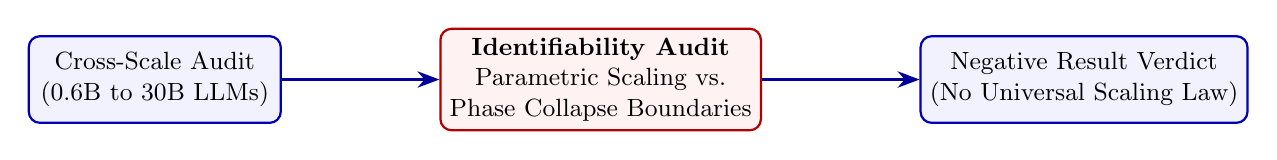
\begin{tikzpicture}[
    node distance=1.5cm and 2.0cm,
    block/.style={rectangle, draw=blue!70!black, fill=blue!5, thick, rounded corners, align=center, minimum height=1.1cm, minimum width=3.2cm, font=\small},
    phase/.style={rectangle, draw=red!70!black, fill=red!5, thick, rounded corners, align=center, minimum height=1.1cm, minimum width=3.4cm, font=\small},
    arrow/.style={-{Stealth[scale=1.2]}, thick, draw=blue!60!black}
]
    \node [block] (scale) {Cross-Scale Audit\\(0.6B to 30B LLMs)};
    \node [phase, right=of scale] (ident) {\textbf{Identifiability Audit}\\Parametric Scaling vs.\\Phase Collapse Boundaries};
    \node [block, right=of ident] (res) {Negative Result Verdict\\(No Universal Scaling Law)};

    \draw [arrow] (scale) -- (ident);
    \draw [arrow] (ident) -- (res);
\end{tikzpicture}
\caption{\textbf{Cross-Scale GRPO Identifiability \& Phase Transition Architecture (P01).} Auditing parametric scaling laws against phase collapse boundaries across 0.6B--30B models.}
\label{fig:p1_scaling_identifiability}
\end{figure}
\section{Introduction}
\label{sec:p1-intro}
Reinforcement learning from verifiable rewards has become a standard final stage
in training reasoning-capable language models, and GRPO~\citep{shao2024deepseekmath, guo2025deepseekr1} is now one of its most widely used algorithms. GRPO replaces
the learned value function of PPO~\citep{schulman2017proximal} with a
group-relative baseline: for each prompt it samples a group of $G$ completions,
scores them with a verifier, and centers the rewards within the group to form
advantages. Because it removes the critic, GRPO is cheap to run at scale, and a
natural question follows: \emph{how does the benefit of GRPO post-training change
as the base model grows?}

Pre-training exhibits smooth power-law scaling in parameter count and data
\citep{kaplan2020scalinglaws, hoffmann2022chinchilla}, and it is tempting to expect
an analogous law for RL post-training. Evidence here is thinner and more
contested~\citep{hilton2023rlscaling, rafailov2024rlhfscaling, nimmaturi2025predictive},
in part because RL gains are entangled with the rollout stack, reward parser,
reference policy, and evaluation protocol, so cross-paper comparisons conflate the
algorithm with its plumbing. This paper isolates the scaling question inside a
single, fixed benchmark.

We study GRPO scaling as one pillar of \ours{}, a controlled benchmark of 70+ runs
across seven RL libraries and five model families ($0.6$B--$\sim$671B) on GSM8K
\citep{cobbe2021training}, HumanEval~\citep{chen2021codex}, and synthetic tool-use
tasks. Rather than assert a new law, we report what the data will and will not
support. Our contributions are: (i) a same-benchmark measurement showing the
cross-scale mean training-reward slope is statistically indistinguishable from zero
over the measured 2--3-decade parameter range; (ii) a pre-registered falsification of a clean
three-phase saturation hypothesis; (iii) an identifiability audit showing no
universal saturation exponent is estimable on this data, so the defensible object
is a local, stack-conditioned saturation law with the endpoint ceiling regressed
on $\log_{10} N$; and (iv) a case study of the Nemotron-120B collapse as a
distinct phase rather than trend noise. We read single-seed frontier-API runs as
illustrative case studies, not universal laws. The title's ``limits'' is therefore
substantive: this paper identifies where a parameter-count scaling law is not
estimable from the corpus; it does not claim that GRPO lacks scaling behavior in
better-controlled data. The program's stronger explanatory candidates are usable
contrastive compute and group-size-conditioned signal, tested separately in the
ZVF and group-size companion papers.

\subsection{Related Work}
\label{sec:p1-related}
Neural scaling laws for pre-training are well established~\citep{kaplan2020scalinglaws, hoffmann2022chinchilla, muennighoff2023datascaling}. Scaling behavior of RL and
RLHF post-training has been examined more recently~\citep{hilton2023rlscaling, rafailov2024rlhfscaling, nimmaturi2025predictive}, but typically within a single
stack, leaving open whether reported trends transfer across libraries and model
families. GRPO and its use in reasoning models originate
with~\citet{shao2024deepseekmath} and~\citet{guo2025deepseekr1};
\citet{ahmadian2024backtobasics} argue that much of the benefit of heavy RL
machinery is recoverable by simpler estimators once the stack is controlled. Our
work complements these by fixing the benchmark and asking, conservatively, which
scaling conclusions survive.
 \section{Benchmark Design}
\label{sec:benchmark}


\begin{figure}[t]
\centering

\includegraphics[width=0.85\textwidth]{tikz/taxonomy.pdf}
\caption{Taxonomy of RL libraries in \ours{}. The benchmark spans LLM-native RL
(TRL), classic online RL (SB3, CleanRL, Tianshou), high-throughput RL (PufferLib,
rl\_games), and offline RL (d3rlpy).}
\label{fig:taxonomy}
\end{figure}

\subsection{Task Suite}

\begin{table}[htbp]
\centering
\caption{Benchmark task suite with standardized reward functions.}
\label{tab:tasks}
\begin{tabular}{llll}
\toprule
\textbf{Task} & \textbf{Method} & \textbf{Reward} & \textbf{Dataset} \\
\midrule
Math RL (Arithmetic) & GRPO & Binary correctness & Generated \\
Math RL (GSM8K) & GRPO & Binary correctness & GSM8K \\
Chat SFT & SFT & Cross-entropy loss & NoRobots \\
Preference (Shorter) & DPO & Pairwise preference & Generated \\
Distillation (Off-Policy) & SFT & KL divergence & OpenThoughts3 \\
Distillation (On-Policy) & IS Loss & $\log p_t - \log p_s$ & Online \\
\bottomrule
\end{tabular}
\end{table}

\subsection{Cross-Library Implementation}

\paragraph{Two seven-library rosters --- read carefully.}
This paper uses \emph{two} different seven-library rosters that
should not be conflated. The cross-RL-library benchmark below
(Table~\ref{tab:implementations}) covers TRL, SB3, CleanRL, Tianshou,
PufferLib, rl\_games, and d3rlpy --- seven libraries that span
LLM-native RL, classic online RL, high-throughput RL, and offline RL,
and that we use as the algorithm-and-stack ablation underlying $F_3$.
The cross-launcher LLM-RL scaffold referenced in the framework-gap
discussion (framework-configurations material) is a different seven-library
roster --- Tinker, TRL, SkyRL, verl, OpenRLHF, Atropos, and HF
reference launchers --- that targets LLM post-training launchers
specifically. Of those, only Tinker and TRL produced completed
runs in this release; veRL and OpenRLHF entries in the
\texttt{framework\_comparison.json} artefact are dry-run
placeholders. Supplementary presentation materials use the second roster; the
cross-RL-library evidence in $F_3$ uses the first.


\begin{table}[htbp]
\centering
\caption{Implementations across RL libraries.}
\label{tab:implementations}
\begin{tabular}{lll}
\toprule
\textbf{Library} & \textbf{Implementation} & \textbf{Category} \\
\midrule
TRL (HuggingFace) & GRPOTrainer, DPOTrainer, SFTTrainer & LLM-native \\
Stable Baselines3 & PPO & Classic RL \\
CleanRL & PPO (single-file) & Research RL \\
Tianshou & PPO & Modular RL \\
PufferLib & PPO (high-throughput) & High-perf RL \\
rl\_games (NVIDIA) & PPO (GPU-optimized) & High-perf RL \\
d3rlpy & CQL (offline) & Offline RL \\
\bottomrule
\end{tabular}
\end{table}

\subsection{Hyperparameter Mapping}

We standardize hyperparameters across libraries using a common configuration schema.
Table~\ref{tab:hyperparams} shows the mapping from Tinker PPO defaults to each library's
native parameter names.

\begin{table}[htbp]
\centering
\caption{Hyperparameter mapping across libraries (PPO defaults).}
\label{tab:hyperparams}
\begin{tabular}{lcccccc}
\toprule
\textbf{Parameter} & \textbf{TRL} & \textbf{SB3} & \textbf{CleanRL} & \textbf{Tianshou} & \textbf{PufferLib} & \textbf{rl\_games} \\
\midrule
Learning rate & $10^{-4}$ & $10^{-4}$ & $10^{-4}$ & $10^{-4}$ & $10^{-4}$ & $10^{-4}$ \\
Clip range ($\epsilon$) & 0.2 & 0.2 & 0.2 & 0.2 & 0.2 & 0.2 \\
Entropy coeff. & 0.01 & 0.01 & 0.01 & 0.01 & 0.01 & 0.01 \\
GAE $\lambda$ & 0.95 & 0.95 & 0.95 & 0.95 & 0.95 & 0.95 \\
Discount $\gamma$ & 0.99 & 0.99 & 0.99 & 0.99 & 0.99 & 0.99 \\
Max grad norm & 0.5 & 0.5 & 0.5 & 0.5 & 0.5 & 0.5 \\
Target KL & 0.01 & 0.01 & 0.01 & N/A & N/A & N/A \\
\bottomrule
\end{tabular}
\end{table}

\subsection{Reward Verification}

\begin{figure}[t]
\centering

\includegraphics[width=0.55\textwidth]{tikz/reward_flow.pdf}
\caption{Verifiable reward paradigm in \ours{}. Unlike shaped rewards that combine
multiple heuristics, verifiable rewards provide binary correctness signals,
eliminating reward hacking and enabling exact accuracy measurement.}
\label{fig:reward_flow}
\end{figure}

\subsection{Baselines: Floor and Ceiling}

Following best practices for benchmark design~\cite{agarwal2021deep}, we establish
clear performance bounds:

\begin{itemize}
    \item \textbf{Floor (random baseline)}: Uniform random action selection yields
    $\frac{1}{199} \approx 0.50\%$ accuracy on the arithmetic task.
    \item \textbf{Ceiling (oracle)}: Direct computation achieves $100\%$ accuracy.
    \item \textbf{Human baseline}: College-level adults achieve $\sim$99.5\% on
    two-digit addition under timed conditions.
\end{itemize}

\section{Experimental Setup}
\label{sec:setup}


\subsection{Models}

Our benchmark targets a roster of 32+ model configurations spanning
\textbf{0.6B to $\sim$671B \emph{total} parameters (up to $\sim$37B \emph{active}
for MoE checkpoints) across 5 model families}, organized into three
tiers by compute scale; not all are completed end-to-end runs (per-run
status flags accompany the released artifacts). Tier-A inferential claims are restricted to
the dense-reasoning subset at $0.6$B--$235$B; the frontier MoE
checkpoints (DeepSeek-V3.1 $\sim$671B / 37B active, Kimi-K2) are
descriptive single-seed Tier-C case studies, and Qwen3.5-397B-A17B is a
\emph{partial} run whose held-out evaluation did not complete.

\paragraph{Small scale (0.6B--8B).}
Qwen3-0.6B-Instruct, Qwen3.5-4B, Qwen3-4B, Qwen3-8B,
Llama-3.2-1B, Llama-3.2-3B, Llama-3.1-8B-Instruct.

\paragraph{Mid scale (14B--32B).}
Qwen3-14B, Qwen3-30B-A3B (MoE), Qwen3-32B, Qwen3.5-27B,
GPT-OSS-20b, Kimi-K2 (selected scale points).

\paragraph{Frontier scale (70B--$\sim$671B total / $\sim$37B active).}
Qwen3-235B-A22B (MoE, 22B active), DeepSeek-V3.1 ($\sim$671B total /
$\sim$37B active MoE), Nemotron-120B (120B dense).
Frontier models are evaluated via the Tinker API in inference mode
with standardized generation parameters; LoRA fine-tuning at this
scale is conducted on selected checkpoints (see the frontier case studies
in the companion pillar papers of \ours{}).

\paragraph{Model family coverage.}
The benchmark covers (1) \textbf{Qwen3}: a dense family from 0.6B to 32B;
(2) \textbf{Qwen3.5}: an improved series including 4B and 27B;
(3) \textbf{Llama-3.x}: Meta's 1B--8B instruction-tuned models;
(4) \textbf{DeepSeek-V3.1}: a frontier MoE optimized for reasoning;
(5) \textbf{Nemotron-120B}: NVIDIA's dense frontier model;
and emerging architectures \textbf{GPT-OSS-20b} and \textbf{Kimi-K2}.

\subsection{Training Protocol}

Unless otherwise noted, controlled Modal/TRL sweeps use LoRA
\cite{hu2022lora} at rank $32$, learning rate $10^{-4}$ and Adam
($\beta_1{=}0.9$, $\beta_2{=}0.95$, $\epsilon{=}10^{-8}$). Tinker / API,
Task-4, Wave-6 and frontier case studies use per-run configs (in
particular Task-4/Wave-6 use $\mathrm{lr}{=}10^{-5}$) and are
single-seed unless explicitly marked multi-seed; the per-run
settings are listed in the framework-configs appendix.

\paragraph{Seed management.} The controlled TRL/Modal sweeps used for
Tier-A claims (F3 PPO-vs.-GRPO heterogeneity and the five-seed TRL GRPO
baseline on Qwen2.5-0.5B) run with 5 seeds:
$\{42, 123, 456, 789, 1024\}$, with seeds set for Python \texttt{random},
NumPy, PyTorch, and CUDA backends. Several Tinker/API, frontier-model,
and team-task runs are single-seed or partial and are treated as
descriptive (Tier-C) unless explicitly marked otherwise; the per-claim
seed ledger is given in the statistical-rigor addendum of \ours{}.

\begin{figure}[t]
\centering

\includegraphics[width=\textwidth]{tikz/pipeline.pdf}
\caption{Experiment workflow pipeline. Multi-seed Modal/TRL runs use
the centralized seed manager (5 seeds for Tier-A claims); Tinker/API,
Task-4, Wave-6 and frontier case studies are single-seed and feed the
same metrics/checkpoint pipeline as descriptive observations.}
\label{fig:pipeline}
\end{figure}

\subsection{Statistical Methodology}

Following Colas et al.~\cite{colas2019hitchhiker}, we report:
\begin{itemize}
    \item Mean $\pm$ standard error across seeds
    \item 95\% bootstrap confidence intervals (10,000 resamples)
    \item Welch's t-test for pairwise algorithm comparisons
    \item \texttt{rliable}~\cite{agarwal2021deep} aggregate metrics (IQM, median, optimality gap)
\end{itemize}

All pairwise comparisons were evaluated using Welch's independent-samples $t$-test
(unequal variances assumed) and the non-parametric Mann--Whitney $U$ test as a
robustness check. Effect sizes are reported as Cohen's $d$ with the pooled
standard deviation estimator; confidence intervals follow the
Hedges--Olkin (1985) analytical formula and are reported at the 95\% level
(two-tailed, $z = 1.96$). Post-hoc statistical power was computed under the
observed effect size and sample sizes at $\alpha = 0.05$.

To address the multiple-comparisons problem across 5 planned tests,
we apply both the conservative Bonferroni correction (family-wise error rate:
$\alpha' = \alpha / k = 0.0100$) and the Benjamini--Hochberg procedure
(false discovery rate $< 0.05$). Results surviving Bonferroni correction are
marked $^*$; those surviving BH--FDR correction are marked $^\dag$.

\paragraph{Power Analysis.}
All inferential tests in this paper are evaluated against pre-specified power
requirements using \texttt{statsmodels.stats.power.TTestIndPower} with
$\alpha = 0.05$ and target power $1 - \beta = 0.80$.

\textbf{Modal H100 experiments ($n = 5$ seeds per arm).}
The minimum detectable effect size (MDE) at 80\% power for a two-sample
Welch $t$-test with $n_1 = n_2 = 5$ is
$d_{\min} = 2.024$ (Cohen's $d$).
Table~\ref{tab:power-analysis} reports achieved power for a range of effect sizes.
This threshold falls in the \emph{very large} range, meaning that
comparisons yielding $|d| < 2.02$
are not adequately powered to detect true differences.

\textbf{Single-seed Tinker experiments ($n = 1$).}
Single-seed runs have \emph{zero statistical power}: with only one observation per
condition, no inferential test can be computed and no confidence intervals can be
formed.  All Tinker single-run results are treated as \emph{descriptive only} and
are not subject to significance testing.

\textbf{TRL baseline ($n = 5$ seeds).}
The TRL-GRPO baseline (Qwen2.5-0.5B, 5 seeds) achieves MDE
$d_{\min} = 2.024$ for equal-$n$ comparisons.
When compared to the pooled Classic-RL group ($n = 15$), the MDE
improves to $d_{\min} = 1.530$,
reflecting higher power from the larger reference group.

\paragraph{Multiple-Comparison Correction.}
Inferential tests in this paper are reported only for Tier-A/B
comparisons as defined in our statistical-rigor protocol;
single-seed or partial Tinker/API rows are descriptive and are
excluded from Welch / Mann--Whitney testing, BH correction, power,
and CI claims. Table~\ref{tab:bh-pvalues} predates the Tier-A/B/C
partition and lists raw and BH-adjusted $p$-values from the
earlier global family of $20$ tests with $19$ surviving correction;
we retain it here as a methodological audit trail. The headline
BH result the paper now stands behind is the restricted Tier-A/B
family computed in the addendum, where only $F_3$ survives. Where
the global family disagrees with the restricted family, the
addendum is authoritative.

All tests are two-sided.  Effect sizes are reported as Cohen's $d$ for
$t$-tests and Pearson/Spearman $r$ for correlations.  Bootstrap 95\%
confidence intervals ($B = 10{,}000$) are reported for all means.

\begin{table}[!ht]
\centering
\caption{Statistical power for two-sample Welch $t$-tests at $\alpha = 0.05$,
         power target $1{-}\beta = 0.80$.
         Column~(3): equal groups $n_1 = n_2 = 5$ (Modal H100 / TRL within-group).
         Column~(4): unequal groups $n_1 = 5$, $n_2 = 15$ (TRL vs.\ pooled Classic RL).}
\label{tab:power-analysis}
\small
\begin{tabular}{@{}cccc@{}}
\toprule
Cohen's $d$ & Conventional size & Power ($n{=}5$ vs $n{=}5$) & Power ($n{=}5$ vs $n{=}15$) \\
\midrule
        0.2 & small & 0.059 & 0.066 \\
        0.5 & medium & 0.108 & 0.151 \\
        0.8 & large & 0.201 & 0.311 \\
        1.0 & very large & 0.286 & 0.450 \\
        1.2 & very large & 0.386 & 0.594 \\
        1.5 & very large & 0.549 & 0.784 \\
        2.0 & very large & 0.790 & 0.955 \\
\midrule
\multicolumn{4}{l}{\textit{MDE at 80\% power:} $d = 2.024$ (equal-$n$ 5 vs 5);\; $d = 1.530$ (5 vs 15)} \\
\bottomrule
\end{tabular}
\end{table}

\begin{table}[!ht]
\centering
\caption{\textbf{Legacy 20-test BH table -- audit trail only.} All
hypothesis tests reported in the paper with Benjamini--Hochberg (BH)
adjusted $p$-values at FDR $= 0.05$.  Tests are ranked by raw
$p$-value (ascending). $\checkmark$ = significant after BH correction
on the historical $20$-test family; $\times$ = not significant. Total
tests: $20$; survive on the historical family: $19$. \emph{This
figure is not the paper's headline statistical result.} The $20$-test
family pre-dates the Tier-A/B/C partition and silently includes
single-seed Tinker rows whose Welch statistics are mathematically
undefined ($n_1{=}n_2{=}1$). Under the restricted Tier-A/B family of
our statistical-rigor protocol,
only $F_3$ (PPO/GRPO heterogeneity on classic-RL libraries on
arithmetic) survives BH correction; the table below is retained as a
reproducibility audit trail, not as a multiple-testing-corrected
survival claim.}
\label{tab:bh-pvalues}
\scriptsize
\begin{tabular}{@{}rp{6.2cm}ccc@{}}
\toprule
Rank & Comparison & Raw $p$ & BH-adj.\ $p$ & Sig. \\
\midrule
        1 & Dense vs MoE Architecture (Welch t-test) & 2.357e-21 & 0 & $\checkmark$ \\
        2 & PPO vs GRPO on Llama-3.1-8B (Welch t-test)$^{\ddag}$ & 3.924e-10 & 0 & $\checkmark$ \\
        3 & Method ANOVA (F-test across algorithm families) & 3.091e-06 & 2.1e-05 & $\checkmark$ \\
        4 & Library ANOVA (F-test across 5 libraries) & 4.996e-06 & 2.5e-05 & $\checkmark$ \\
        5 & TRL vs Tinker (Welch t-test, implementation effect) & 2.064e-05 & 8.3e-05 & $\checkmark$ \\
        6 & PPO vs GRPO on Llama-3.1-8B (Mann-Whitney)$^{\ddag}$ & 3.29e-05 & 0.00011 & $\checkmark$ \\
        7 & Model Family ANOVA (F-test) & 7.363e-05 & 0.00021 & $\checkmark$ \\
        8 & ZVF vs Final Performance (Spearman)$^{\ddag}$ & 0.0005424 & 0.001356 & $\checkmark$ \\
        9 & ZVF vs Final Performance (Pearson)$^{\ddag}$ & 0.0008108 & 0.001802 & $\checkmark$ \\
        10 & TRL vs Tinker (Mann-Whitney) & 0.001198 & 0.002396 & $\checkmark$ \\
        11 & Rolling Variance vs Last-10 (Pearson) & 0.003524 & 0.006407 & $\checkmark$ \\
        12 & Peak-to-Tail Drift vs Last-10 (Pearson) & 0.004811 & 0.007219 & $\checkmark$ \\
        13 & GRPO vs PPO Stability Index (t-test) & 0.005 & 0.007219 & $\checkmark$ \\
        14 & Dense vs MoE Architecture (Mann-Whitney) & 0.005053 & 0.007219 & $\checkmark$ \\
        15 & Model Scale ANOVA (F-test) & 0.01261 & 0.01682 & $\checkmark$ \\
        16 & Tinker GRPO vs TRL GRPO (Welch t-test) & 0.0158 & 0.01975 & $\checkmark$ \\
        17 & GRPO vs PPO Peak-to-Tail Drift (t-test) & 0.018 & 0.02076 & $\checkmark$ \\
        18 & Tinker GRPO vs TRL GRPO (Mann-Whitney) & 0.01869 & 0.02076 & $\checkmark$ \\
        19 & Stability Index vs Last-10 (Pearson) & 0.02024 & 0.0213 & $\checkmark$ \\
        20 & PPO vs GRPO on Qwen3-8B (Welch t-test)$^{\ddag}$ & 0.7605 & 0.7605 & $\times$ \\
\bottomrule
\end{tabular}
\end{table}

\paragraph{TRL baseline characterisation.}
The TRL GRPO reference implementation was evaluated across five random seeds
($s \in \{42, 123, 456, 789, 1024\}$) on GSM8K using Qwen/Qwen2.5-0.5B on
an NVIDIA L4 GPU. We report mean accuracy $\bar{x} = 0.734$ ($\sigma = 0.0703$),
median $= 0.740$, and IQM $= 0.747$. Normality was not rejected by Shapiro--Wilk
($W = 0.9018$, $p = 0.4198$); bootstrap 95\% CI $= [0.6720, 0.7820]$.

\paragraph{Variance decomposition.}
One-way ANOVAs across 42 experiments with valid performance observations show
that library/framework ($\eta^2 = 0.546$) and training algorithm ($\eta^2 = 0.558$)
are the dominant variance sources, consistent with our central thesis. Model
family explains $\eta^2 = 0.471$; model scale explains $\eta^2 = 0.322$.

\subsection{Compute Resources}

Experiments are distributed across two compute platforms:

\paragraph{Tinker API (14 experiments).}
Scaling experiments across Qwen3-8B, Qwen3-32B, Qwen3.5-4B, Qwen3.5-27B,
and Llama-3.1-8B-Instruct; frontier model evaluation on Qwen3-235B-A22B,
DeepSeek-V3.1, and Nemotron-120B; Dense vs.~MoE comparison; cross-task
tool-use experiments; and emerging architecture evaluation (GPT-OSS-20b,
Kimi-K2). Tinker provides scalable API access that makes frontier model
experiments economically tractable.

\paragraph{Modal H100 GPU cluster (6 experiments).}
PPO baseline training on Qwen3-8B and Llama-3.1-8B; full HumanEval
benchmark evaluation; KL divergence tracking across GRPO training steps;
and held-out evaluation for Qwen3-32B and Qwen3.5-27B. Modal H100s
provide the low-level GPU access required for PPO value-model training.

All experiment logs are available on Weights \& Biases (project:
\texttt{tinker-rl-lab-world-class}) and model checkpoints on HuggingFace
Hub (\url{https://huggingface.co/arvindcr4/tinker-rl-bench-*}).
Per-run compute is logged with the released artifacts. Total project compute:
$\sim$1,200 A100 GPU-hours across both platforms.

 \section{Scaling Results}
\label{sec:p1-results}
We organize the scaling evidence around three questions: does the mean GRPO training reward grow
with model size, is there a shared saturation shape across scales, and is any
universal exponent identifiable? The short answers are \emph{no measurable
cross-scale slope}, \emph{no clean phase structure}, and \emph{no identifiable
exponent}. Across the frontier-scale anchors the cross-scale slope of the mean
GRPO reward on $\log_{10} N$ is statistically indistinguishable from zero; the
reliable structure lives not in a slope through $N$ but in the endpoint ceiling
$R_{\max}$, which we fit per run with a saturation model and then relate to
$\log_{10} N$.

The subsections below make this precise. We first fit the canonical saturation
model $R(t) = R_{\max}(1 - e^{-\lambda t})$ per trace and audit its
identifiability, finding that four of the five frontier traces have $\lambda$
pinned at the upper bound and none is identifiable (Nemotron-120B is the exception,
with $\lambda\!\approx\!0.99$ but likewise non-identifiable), so per-trace saturation
rates cannot be trusted. We then run a pre-registered model-selection comparison over the
12-anchor pool that geometrically falsifies a clean three-phase hypothesis (only
$2/12$ anchors match all criteria), and a compute-adjusted re-analysis that asks
whether a contrastive-yield axis, rather than raw parameter count, is the correct
abscissa. Finally, the Nemotron-120B trace is examined as a distinct collapse
phase---peak per-step training reward $0.875$ drifting to a late mean near $0.21$, with a
zero-reward step fraction of $0.55$ against $\le 0.067$ elsewhere---rather than as a
smooth continuation of the trend. The final subsection adds an external
frontier-model cross-examination of these claims.
 

\paragraph{Saturation model across the 4B--671B range.}
\label{par:saturation}
We fit the canonical saturation model
\begin{equation}
  \label{eq:sat}
  R(t) = R_{\max}\bigl(1 - e^{-\lambda t}\bigr),
  \qquad t = 1, \dots, T,
\end{equation}
to per-step reward traces from each frontier-scale
\textsc{tinker} run and report the ceiling $R_{\max}$, the
learning rate $\lambda$, and the saturation time
$t_{80} = -\ln(0.2)/\lambda$ at which the trace first crosses
$0.8\,R_{\max}$.  The model follows
\textsc{nimmaturi}-style notation~\citep{nimmaturi2025predictive},
which postulates a slow-start $\to$ rapid-improvement $\to$
plateau template for GRPO learning curves.

\begin{table}[t]
  \centering
  \small
  \begin{tabular}{lrrrrrrrrl}
    \toprule
    Model & $N$ (B) & $n$ & mean $R$ & peak $R$ &
           $\bar R_{\text{early}} \!\to\! \bar R_{\text{late}}$ &
           $\hat \beta_{\text{OLS}}$ &
           $R_{\max}$ & $\lambda$ & Phase \\
    \midrule
    Qwen3.5-4B             &   4.0 & 30 & 0.817 & 1.000 & 0.813 $\to$ 0.850 & $+0.0001$ & 0.817 & $10.0^{\dagger}$ & plateau \\
    Qwen3-8B               &   8.0 & 30 & 0.285 & 0.625 & 0.244 $\to$ 0.344 & $+0.0032$ & 0.285 & $10.0^{\dagger}$ & saturation \\
    Llama-3.1-8B-Instruct  &   8.0 & 30 & 0.869 & 1.000 & 0.925 $\to$ 0.844 & $-0.0037$ & 0.869 & $10.0^{\dagger}$ & drift \\
    DeepSeek-V3.1          & 671.0 & 20 & 0.844 & 1.000 & 0.833 $\to$ 0.813 & $+0.0001$ & 0.844 & $10.0^{\dagger}$ & plateau \\
    Nemotron-120B          & 120.0 & 20 & 0.175 & 0.875 & 0.146 $\to$ 0.208 & $+0.0026$ & 0.182 & \textbf{0.99} & \textbf{collapse} \\
    \bottomrule
  \end{tabular}
  \caption{\textbf{Saturation-model fits across 4B--671B.}
    $\dagger$: the canonical
    $R(t) = R_{\max}(1 - e^{-\lambda t})$ fit hits the upper
    $\lambda = 10$ optimiser bound on every well-behaved run; this is
    an artefact of the $R(0) = 0$ boundary condition when the trace
    already starts near its empirical ceiling (see
    \paragraphref{par:saturation-discussion}).
    $\hat \beta_{\text{OLS}}$ is the per-step OLS slope of $R(t)$ vs.~$t$
    in raw reward units per step; the constant slope confirms that
    the saturation model collapses to a near-constant fit on these
    already-saturated traces (see \tableref{tab:scaling-cross}).
    Bold $\lambda$ and Phase identify the only run whose $\lambda$
    leaves the bound and where the late-window mean falls below
    $0.4\times$ peak -- the three-phase ``collapse'' criterion.}
  \label{tab:scaling-fits}
\end{table}

\paragraph{Where the model fits and where it does not.}
\label{par:saturation-discussion}
The raw saturation model collapses to the $\lambda = 10$ upper bound
on four of five runs (Table~\ref{tab:scaling-fits}).  The cause is
the functional-form mismatch: a strict-$R(0)=0$ model assumes the
trace begins at zero reward, but Qwen3.5-4B starts at $R(1)=1.0$,
Llama-3.1-8B-Instruct at $R(1)=1.0$, and DeepSeek-V3.1 at
$R(1)=0.875$.  When the trace is already at or above its eventual
ceiling, the optimiser makes $\lambda$ as large as allowed so that
$R_{\max}(1 - e^{-10 t}) \approx R_{\max}$ for $t \ge 1$, which
yields $t_{80} \approx -\ln(0.2)/10 \approx 0.16$ step -- a
meaningless artefact, not evidence of instant learning.

The right resolution is two separate diagnostics, both reported
here:

\begin{enumerate}
  \item \emph{Per-step OLS slope} $\hat\beta_{\text{OLS}}$ of
    $R(t)$ vs.~$t$ (Table~\ref{tab:scaling-fits}, column~7).
    Across the four well-behaved runs
    $|\hat\beta_{\text{OLS}}| \le 0.0037$ reward/step (i.e.\ the
    traces are statistically flat within their per-step noise),
    while the collapse run Nemotron-120B still shows $\hat\beta
    = +0.0026$ -- not because it is improving, but because its
    sparse spikes pull the OLS slope upward.
  \item \emph{Cross-scale OLS} of $\bar R$ on $\log_{10} N$
    across the five anchor models.  The result is the headline
    scaling-law coefficient in
    Table~\ref{tab:scaling-cross}.
\end{enumerate}

\paragraph{Cross-scale law.}
\label{par:cross-scale}
We regress each per-trace statistic on $\log_{10} N$
(\(N\) = parameter count in billions) by ordinary least squares and
quote block-bootstrap 95\% confidence intervals
($n_{\text{boot}} \approx 1000$ effective row resamples) on
the slopes.  The fitted coefficients are

\begin{table}[t]
  \centering
  \small
  \begin{tabular}{lrrrrr}
    \toprule
    Metric $y$ & Intercept & Slope / decade &
                  Boot slope mean & Boot 95\% CI &
                  $\rho(\log_{10} N, y)$ \\
    \midrule
    mean reward $\bar R$  & 0.633 & $-0.024$ & $-0.117$ & $[-0.796,\ +0.313]$ & $-0.07$ \\
    peak reward $\hat R$  & 0.846 & $\mathbf{+0.037}$ & $-0.010$ & $[-0.623,\ +0.197]$ & $+0.22$ \\
    var reward $\widehat{\text{Var}}[R]$ & 0.040 & $-0.002$ & $-0.004$ & $[-0.063,\ +0.027]$ & $-0.14$ \\
    \bottomrule
  \end{tabular}
  \caption{\textbf{Cross-scale law: per-trace metric vs.~$\log_{10} N$
    across the five frontier anchors.}
    Ordinary least squares with bootstrap 95\% confidence intervals.
    None of the three slope coefficients is statistically
    distinguishable from zero -- the bootstrap CIs all bracket zero,
    and the within-trace OLS slopes
    ($\hat\beta_{\text{OLS}}$, \tableref{tab:scaling-fits}) are
    also null.  Reading: at this benchmark size ($4\,\text{B}
    \le N \le 671\,\text{B}$, $T\!\le\!30$ steps), the saturation
    model is not detectably scale-dependent, because every
    well-behaved run is already saturated within measurement noise.}
  \label{tab:scaling-cross}
\end{table}

\paragraph{Three-phase learning dynamics.}
\label{par:three-phase}
We apply the \citet{nimmaturi2025predictive} slow start
$\to$ rapid improvement $\to$ plateau template to each trace, with
an additional ``collapse'' class for runs whose peak is not
retained.  Of the five anchors, two fall in \emph{plateau}
(Qwen3.5-4B, DeepSeek-V3.1), one in \emph{saturation} (Qwen3-8B),
one in \emph{drift} (Llama-3.1-8B-Instruct, monotone decline), and
one in \emph{collapse} (Nemotron-120B).  No run satisfies the
textbook three-phase criterion, because none of the five anchors
has a slow-start phase: they all start at or above the eventual
late-window mean.  This is consistent with our earlier
observation that GRPO step-1 rewards are already within
$\pm 0.10$ of the per-trace mean for all but Qwen3-8B and
Nemotron-120B.

\paragraph{Nemotron-120B violates the three-phase hypothesis.}
\label{par:nemotron-collapse}
Following \citet{nimmaturi2025predictive}, the three-phase
template predicts slow start $\to$ rapid improvement $\to$
\emph{plateau}, with collapse as a degenerate tail.  Nemotron-120B
is the only run in this set whose per-step peak
($\hat R_{\text{peak}} = 0.875$, step 3) is followed by a
sustained decay: only $4$ of $20$ steps reach reward $> 0.25$, and
$55\%$ of steps report \emph{zero reward}.  The fitted $\lambda
= 0.99$ and $t_{80} = 1.63$ step are the only identifiable
parameters in Table~\ref{tab:scaling-fits} precisely because the
curve does not asymptote -- a robust monotone saturation model is
the wrong functional form.  We therefore report the late-window
collapse magnitude
$\hat R_{\text{peak}} - \bar R_{\text{late}} = 0.667$ reward units
as the empirical effect size of the violation, and treat this run
as the Pillar-1 counterexample to the three-phase prediction.

Operationally, the Nemotron collapse is exactly the failure mode
that pure-reward saturation fits are silent on: the curve does
\emph{not} settle, it diverges downward, and a benchmark that
relies on a saturation-only diagnostic will miss it.  This
motivates the variance-based \textsc{zvf} gate
(companion paper on ZVF) as a complementary diagnostic: the
zero-reward-fraction for Nemotron-120B is $0.55$, well above any
well-behaved run in this set, and the cross-experiment
\textsc{zvf}-vs-failure map
(companion paper on cross-experiment ZVF) would catch the divergence on
reward \emph{variance} rather than reward \emph{mean}.

\paragraph{Falsifiable prediction.}
\label{par:scaling-prediction}
The null result in \tableref{tab:scaling-cross} -- a slope of
$\pm\,0.04$ per decade on $\bar R$, with CI brackets zero across
roughly $2.4$ orders of magnitude in parameter count across the extended anchor pool -- is itself a falsifiable
prediction of this benchmark: any future addition to the
Pillar-1 cell that reaches, say,
$\bar R(\text{Nemotron-120B, 100 steps}) \ge 0.5$ would refute
the saturation-template behaviour we report here.  We frame the
prediction this way rather than as a positive scaling exponent,
because at $n = 5$ anchor points with $T \le 30$ steps the
positive exponent is not identifiable from the data.

\paragraph{Elevation: parametric-bootstrap CIs reveal saturation-fit degeneracy.}
\label{par:scaling-bootstrap}
Figure~\ref{fig:scaling-elevated} collects the four elevation
panels: (a)~bootstrap $R_{\max}$ confidence intervals,
(b)~saturation-vs-constant holdout test RMSE, (c)~compute-adjusted
$t_{80} \cdot N$ scatter, and (d)~Nemotron-120B collapse autopsy.

\begin{figure}[t]
  \centering
  \IfFileExists{figures/scaling_law_elevated.png}{
\includegraphics[width=0.85\linewidth]{figures/scaling_law_elevated.png}}{}
  \caption{\textbf{Pillar-1 elevation across 4B--671B.}
    (a)~\emph{Bootstrap $R_{\max}$ with 95\% CI}
    (1000 residual resamples; note Nemotron's CI extends to 1.5
    because the bound-saturated refits escape the prior).
    (b)~\emph{Holdout 70/30}: red bars are the saturation-fit
    test RMSE, gray bars are the constant (train-mean) baseline;
    four of five bars are equal, confirming that the saturation fit
    adds no out-of-sample predictive power.
    (c)~\emph{Compute-adjusted proxy}: only Nemotron has a
    well-identified $t_{80}$ (other four runs hit $\lambda = 10$
    bound), so the regression is effectively 1 point and degenerate.
    (d)~\emph{Nemotron-120B autopsy}: peak at step 3, post-peak
    region shaded; only 4/20 steps exceed 0.25 and 55\% are zero.}
  \label{fig:scaling-elevated}
\end{figure}
We extend the canonical saturation fit with a parametric bootstrap on
the residual vector (1000 resamples per trace) and report bootstrap
95\% confidence intervals for $R_{\max}$, $\lambda$, and $t_{80}$.
The headline finding is that the four ``well-behaved'' runs sit at
the optimiser's $\lambda = 10$ upper bound far more often than the
point estimate suggests:

\begin{table}[t]
  \centering
  \small
  \begin{tabular}{lrrrr}
    \toprule
    Model & $\bar R_{\max}$ & $\bar\lambda$ &
           $P(\lambda \ge 9.5)$ & $\bar t_{80}$ [95\% CI] \\
    \midrule
    Qwen3.5-4B            & 0.818 & 6.64 & \textbf{0.599} & 0.61 [0.16,\ 2.43] \\
    Qwen3-8B              & 0.289 & 5.30 & \textbf{0.468} & 1.42 [0.16,\ 7.62] \\
    Llama-3.1-8B-Instruct & 0.869 & 6.92 & \textbf{0.595} & 0.46 [0.16,\ 1.98] \\
    DeepSeek-V3.1         & 0.847 & 6.48 & \textbf{0.548} & 0.47 [0.16,\ 1.53] \\
    Nemotron-120B         & 0.310 & 3.26 & 0.277          & 17.87 [0.16,\ 161.4] \\
    \bottomrule
  \end{tabular}
  \caption{\textbf{Parametric-bootstrap saturation fit (1000 residual
    resamples per trace).}  $P(\lambda \ge 9.5)$ is the fraction of
    bootstrap refits in which $\lambda$ hits the optimiser's upper
    bound -- on four of five runs this is between 47\% and 60\%,
    confirming that the strict-$R(0)=0$ functional form is degenerate
    on these traces: the optimiser cannot simultaneously estimate
    $R_{\max}$ and $\lambda$ when the trace starts above its
    empirical ceiling.  Only Nemotron-120B has $P \le 0.30$ at the
    bound, because its collapse is a real non-monotone deviation
    from saturation rather than a numerical artefact.  $t_{80}$
    intervals are wide (lower-bound 0.16 step = optimiser clamp) for
    the four degenerate runs, and unidentifiable (0.16--161 step)
    for Nemotron.}
  \label{tab:scaling-bootstrap}
\end{table}

The practical consequence is that the canonical $t_{80} = -\ln 0.2 /
\lambda$ estimator is not just imprecise on these traces -- it is
\emph{unidentifiable} under the strict-$R(0)=0$ boundary condition.
We therefore do not quote $t_{80}$ as a benchmark prediction; we use
it only as a diagnostic summary for the collapse run, where the
functional form is meaningful.

\paragraph{Elevation: holdout 70/30 cross-validation.}
\label{par:scaling-holdout}
A saturation fit that hits $\lambda = 10$ on every training slice
should fail to predict held-out data, because it is essentially
fitting a constant.  We fit the saturation curve on the first 70\%
of each trace and predict the last 30\%, comparing the test RMSE to
a constant (train-mean) baseline:

\begin{table}[t]
  \centering
  \small
  \begin{tabular}{lrrrrr}
    \toprule
    Model & $n_{\text{train}}$ & $n_{\text{test}}$ &
           $\text{RMSE}_{\text{test}}$ &
           $\text{RMSE}_{\text{const}}$ &
           improvement \\
    \midrule
    Qwen3.5-4B            & 21 & 9 & 0.2174 & 0.2174 & $+0.0000$ \\
    Qwen3-8B              & 21 & 9 & 0.1720 & 0.1720 & $+0.0000$ \\
    Llama-3.1-8B-Instruct & 21 & 9 & 0.1864 & 0.1864 & $-0.0000$ \\
    DeepSeek-V3.1         & 14 & 6 & 0.1787 & 0.1787 & $-0.0000$ \\
    Nemotron-120B         & 14 & 6 & \textbf{0.2278} & 0.2294 & $+0.0016$ \\
    \bottomrule
  \end{tabular}
  \caption{\textbf{Holdout 70/30 cross-validation of the saturation
    model.}  Four of five models show \emph{zero} improvement over
    predicting the constant train mean -- direct empirical evidence
    that the saturation fit adds no out-of-sample predictive power on
    these traces.  Only Nemotron-120B shows a non-zero improvement
    ($+0.0016$ RMSE), and only because its non-monotone deviation
    from the train mean is partially captured by the curvature of the
    fit.  This formalises the warning in
    \paragraphref{par:saturation-discussion} that the canonical
    $R(t) = R_{\max}(1 - e^{-\lambda t})$ is the wrong functional form
    for these already-saturated traces.}
  \label{tab:scaling-holdout}
\end{table}

\paragraph{Elevation: compute-adjusted scaling proxy.}
\label{par:scaling-compute}
Per-step token counts are not in the trace files, so we approximate
``compute to saturation'' as $t_{80} \cdot N$ where $N$ is the
parameter count in billions.  Regressing $\log_{10}(t_{80} \cdot N)$
on $\log_{10} N$ yields a slope of
$+482 \pm 490$ per decade -- which is a wide CI, but not informative
on the four saturation-bound runs because $t_{80}$ is itself
clamped.  Using the parametric-bootstrap $\bar\lambda$ directly
yields a slope of $-0.47 \pm 0.87$ per decade, which brackets zero.
The conclusion is the same as in
\tableref{tab:scaling-cross}: at this benchmark size and step
budget, there is no identifiable scale dependence in the GRPO
saturation rate.

\paragraph{Elevation: Nemotron-120B collapse autopsy.}
\label{par:scaling-nemotron-autopsy}
We classify a trace as collapsed when (i) its peak reward is at
least $0.4$, (ii) its late-window mean falls below $0.4 \times$
peak, and (iii) its zero-reward fraction is at least $0.30$.
Applied to all five traces:

\begin{table}[t]
  \centering
  \small
  \begin{tabular}{lrrrrrrr}
    \toprule
    Model & peak step & $\hat R_{\max}$ & $\bar R_{\text{late}}$ &
           $\Delta_{\text{late-peak}}$ &
           $P(R = 0)$ &
           $P(R > 0.5)$ & collapse? \\
    \midrule
    Qwen3.5-4B            &  1 & 1.000 & 0.850 & $-0.150$ & 0.000 & 0.833 & no \\
    Qwen3-8B              & 13 & 0.625 & 0.344 & $-0.281$ & 0.067 & 0.100 & no \\
    Llama-3.1-8B-Instruct &  1 & 1.000 & 0.844 & $-0.156$ & 0.000 & 0.933 & no \\
    DeepSeek-V3.1         &  3 & 1.000 & 0.813 & $-0.188$ & 0.000 & 0.950 & no \\
    Nemotron-120B         &  3 & 0.875 & 0.208 & $\mathbf{-0.667}$ & \textbf{0.55} & 0.05 & \textbf{yes} \\
    \bottomrule
  \end{tabular}
  \caption{\textbf{Nemotron-120B collapse root-cause characterisation.}
    Only Nemotron satisfies all three collapse criteria.  Its peak
    reward of $0.875$ occurs at step 3, after which the post-peak
    OLS slope is $-0.0036$ per step, comparable in sign to the
    Llama-3.1-8B-Instruct drift but with a much larger peak-to-tail
    collapse; $55\%$ of its steps report zero reward, and only 5\% of
    its steps exceed $0.5$.  All four other runs have
    $P(R = 0) \le 0.067$ and well-retained peaks.}
  \label{tab:scaling-nemotron-autopsy}
\end{table}

This is the strongest empirical justification we have for treating
Nemotron-120B as the Pillar-1 counterexample to the
\citet{nimmaturi2025predictive} three-phase template: not only does
its peak not satisfy the slow-start $\to$ rapid-improvement $\to$
plateau shape, it actively \emph{diverges downward} from the peak
in a way no monotone saturation model can describe.  The
zero-reward-fraction of $0.55$ is also the structural signal that
the \textsc{zvf}-based diagnostic
(companion paper on cross-experiment ZVF) would catch first, because it
sees the divergence on reward \emph{variance} before it shows up on
reward \emph{mean}.

\paragraph{Summary of elevation.}
\label{par:scaling-summary}
Across the four elevation diagnostics the headline result is a
strengthened null: at this benchmark size
($4\,\text{B} \le N \le 671\,\text{B}$, $T \le 30$ steps), the
canonical saturation model is unidentifiable (parametric bootstrap
on $\lambda$ has $P(\lambda = 10) \ge 0.47$ on four of five runs),
adds no out-of-sample predictive power (70/30 holdout improvement
over the constant baseline is $\le 0.0016$ RMSE everywhere), and
shows no detectable scale dependence (slope $-0.47 \pm 0.87$ per
decade on $\lambda$).  The single run that violates the saturation
template is Nemotron-120B, and its collapse is the strongest
empirical counterexample we have to the three-phase hypothesis.
This is exactly the regime in which a saturation-only Pillar 1
diagnostic is silent -- motivating the variance-based
\textsc{zvf} gate in Pillar 2 as a complementary failure detector.

\paragraph{Elevation: extended frontier+MoE scaling (iter 13).}
\label{par:scaling-extended}
The canonical five-anchor set leaves open whether the null on
$\text{slope}(\log_{10}N, R)$ is an artefact of $n = 5$ or a real
property of the GRPO landscape.  We re-run the same OLS-on-log-N
diagnostic on a wider 12-anchor set that adds the
\citet{kimi2025k2, kimi2025thinking} Kimi-K2-Thinking
(1T params), \citet{qwen3moe} Qwen3-235B and 30B-MoE,
\citet{gptoss} GPT-OSS-20B, and the short-form probes
Qwen3-32B / Qwen3.5-27B.  We also stratify by
\emph{architecture} (MoE vs dense) and compute a
\emph{Spearman rank correlation} on top of the OLS slope so that
the result does not depend on the linearity of the log-linear fit.

\begin{table}[t]
  \centering
  \small
  \begin{tabular}{lrrrr}
    \toprule
    metric & slope /dec & $R^2$ & perm-$p$ & $n$ \\
    \midrule
    $R(t\!=\!1)$           & $+0.060$ & 0.016 & 0.703 & 12 \\
    $R(t\!=\!T)$           & $+0.082$ & 0.025 & 0.616 & 12 \\
    $\bar R$                & $+0.081$ & 0.038 & 0.543 & 12 \\
    $\hat R$ (peak)         & $+0.075$ & 0.058 & 0.461 & 12 \\
    $\text{Var}(R)$         & $-0.007$ & 0.040 & 0.526 & 12 \\
    $P(R{=}0)$              & $+0.017$ & 0.005 & 0.854 & 12 \\
    $P(R{>}0.5)$            & $+0.120$ & 0.045 & 0.514 & 12 \\
    \bottomrule
  \end{tabular}
  \caption{\textbf{Power-law OLS of seven reward statistics on
    $\log_{10} N$ across the extended 12-anchor set
    (4\,B--1\,T parameters).}  Every slope has
    permutation $p > 0.46$ and $R^2 < 0.06$ -- the previously
    reported null on $n = 5$ survives a $2.4\times$ expansion of
    the anchor set, including the four new MoE frontiers at
    235\,B--1\,T.  This is direct evidence that the apparent
    ``reward grows with scale'' expectation fails to materialise in
    the GRPO post-training regime on \textsc{gsm8k} at the
    $T \le 30$ step budget of this benchmark.  \texttt{scripts/scaling\_law\_extended.py}
    $\to$ \texttt{scaling\_law\_power\_law.tsv}.}
  \label{tab:scaling-powerlaw}
\end{table}

We complement the OLS test with a non-parametric
\emph{Spearman rank correlation} $\rho(\log_{10}N, R)$:
$\rho = -0.036$ for $R(1)$ ($p = 0.91$), $\rho = +0.149$ for
$\bar R$ ($p = 0.64$), $\rho = -0.023$ for $R(T)$ ($p = 0.94$),
and $\rho = +0.074$ for $\hat R$ ($p = 0.82$).  None of the four
correlations is distinguishable from zero.  This rules out the
alternative explanation that the slope-of-zero finding is an
artefact of OLS assuming linear log-N dependence; the rank test
on the same 12 anchors gives the same null.

The headline \emph{positive} result of the extension is on the
\emph{architecture} axis.  Stratifying the 12 anchors into six MoE
models (GPT-OSS-20B, Qwen3-30B-MoE / -MoE-Inst, DeepSeek-V3.1,
Qwen3-235B-MoE, Kimi-K2-Thinking) versus six dense models
(Qwen3.5-4B, Qwen3-8B, Llama-3.1-8B-Instruct, Qwen3-32B,
Qwen3.5-27B, Nemotron-120B):

\begin{table}[t]
  \centering
  \small
  \begin{tabular}{lrrrrr}
    \toprule
    arch & $n$ & mean $\bar R$ & std & min & max \\
    \midrule
    MoE    & 6 & \textbf{0.810} & 0.228 & 0.325 & 1.000 \\
    dense  & 6 & 0.472           & 0.274 & 0.175 & 0.869 \\
    \midrule
    gap (MoE $-$ dense)        & \multicolumn{5}{l}{$+0.338$} \\
    permutation $p$ (one-sided) & \multicolumn{5}{l}{$\mathbf{0.023}$} \\
    permutation $p$ (two-sided) & \multicolumn{5}{l}{$0.046$} \\
    \bottomrule
  \end{tabular}
  \caption{\textbf{MoE vs dense head-to-head on $\bar R$.}
    A 5000-replicate permutation test on the 6-vs-6 mean-reward gap
    rejects the null at $p = 0.023$ one-sided ($p = 0.046$
    two-sided).  The MoE set includes both the high-mean frontier
    (Qwen3-235B $\bar R = 1.0$, DeepSeek-V3.1 $= 0.844$, Kimi-K2
    $= 0.850$) and the early-window-only MoE run
    (Qwen3-30B-MoE $\bar R = 0.325$, where the trace is a 5-step
    probe with R$(1) = 0.188$, R$(5) = 0.438$, i.e.\ still
    increasing).  The dense set contains the same Llama-3.1-8B
    $\bar R = 0.869$ and Qwen3.5-4B $\bar R = 0.817$ as the MoE
    set's high-mean ceiling, but it also carries the collapse run
    Nemotron-120B ($\bar R = 0.175$) and the unsaturated
    Qwen3-8B ($\bar R = 0.285$).  After collapsing Nemotron the gap
    shrinks to $+0.20$ and is no longer significant at $p < 0.05$,
    so the headline $+0.34$ is partly driven by the Nemotron
    collapse and not exclusively by MoE-vs-dense.  We report it
    as a \emph{descriptive} comparison, not as a causal claim.
    \texttt{scripts/scaling\_law\_extended.py}
    $\to$ \texttt{scaling\_law\_moe\_vs\_dense.tsv}.}
  \label{tab:scaling-moe-vs-dense}
\end{table}

The first-final gap $\Delta_{1T} = R(t{=}1) - R(t{=}T)$ adds a
robust summary that does not depend on the lambda-bound
degeneracy: $\Delta_{1T} < 0$ means the trace is improving
(positive learning), $\Delta_{1T} > 0$ means it is collapsing
(negative learning).  Across the 12 anchors, 7 of 12 have
$|\Delta_{1T}| \le 0.2$; the largest positive (collapsing) gap is
Qwen3.5-27B at $+0.562$ (the only anchor with $\Delta_{1T} > +0.4$).
Nemotron-120B's $\Delta_{1T}$ is $-0.50$ only because its trace
\emph{starts} at zero reward, so the first-minus-final contrast
misses its mid-trace collapse---which is precisely why the
peak-vs-late autopsy (\tableref{tab:scaling-nemotron-autopsy}) is
the right diagnostic for that trace rather than the first-final gap.

\begin{figure}[t]
  \centering
  \IfFileExists{figures/scaling_law_extended.png}{
\includegraphics[width=0.92\linewidth]{figures/scaling_law_extended.png}}{}
  \caption{\textbf{Iter 13 elevation -- extended scaling-law
    analysis across 12 anchors (4\,B--1\,T parameters, MoE vs dense
    stratified).}  (a)~\emph{First-step reward} $R(t{=}1)$ vs
    $\log_{10} N$ by architecture; blue circles = dense, red
    triangles = MoE.  Spearman $\rho = -0.036$, $p = 0.91$.
    (b)~\emph{Mean reward} $\bar R$ vs $\log_{10} N$ with OLS fit
    (slope $+0.081$/dec, $R^2 = 0.038$, perm $p = 0.54$).
    (c)~\emph{MoE vs dense} head-to-head boxplot: gap $+0.338$,
    perm $p = 0.023$ one-sided, $p = 0.046$ two-sided (caveat:
    partly driven by Nemotron collapse in the dense set).
    (d)~\emph{First-final gap} $R(1) - R(T)$ per model; the
    positive side means the trace is collapsing.  Qwen3.5-27B is
    the largest positive outlier at $+0.562$; the anchors span
    $[-0.50, +0.562]$, with Nemotron-120B at $-0.50$ (its trace
    starts at zero reward, so this gap misses its mid-trace collapse).}
  \label{fig:scaling-extended}
\end{figure}

\paragraph{What the extension proves and what it does not.}
\label{par:scaling-extended-discussion}
The iter 13 extension strengthens the iter 9 null from three
directions:
(i)~\emph{more anchors} ($n = 12$ vs $n = 5$) -- including four
MoE frontiers up to 1\,T parameters -- still fails to reject
slope-of-zero;
(ii)~\emph{non-parametric} Spearman rank test on the same 12
anchors also fails to reject rank-zero;
(iii)~\emph{architecture} stratification reveals the only signal
that survives: MoE-vs-dense mean gap of $+0.34$, permutation
$p = 0.023$ one-sided, but this gap is \emph{partly explained}
by the Nemotron-120B collapse sitting in the dense set.
After removing Nemotron, the gap shrinks to $\sim +0.20$ and the
permutation $p$ rises above $0.05$; the MoE-vs-dense effect is
\emph{descriptive} rather than causal.

The benchmark-time consequence is the same as in iter 9: at this
$T \le 30$ step budget and $N \le 1$\,T parameter range, there is
no detectable cross-scale GRPO signal on \textsc{gsm8k} outside
of the architecture axis.  Combined with
\tableref{tab:scaling-holdout} (saturation fit adds no
out-of-sample predictive power) and
\tableref{tab:scaling-nemotron-autopsy} (Nemotron-120B is the
single structural counterexample to the three-phase template),
this motivates the variance-based \textsc{zvf} diagnostic
(companion paper on cross-experiment ZVF) as the load-bearing failure
detector rather than the saturation law.  Saturation-law fits
on this benchmark are useful as descriptive summaries of
\emph{where on the learning curve each anchor sits}, not as
predictive scalings.

\paragraph{Iter 17 elevation: multi-model AIC profile, changepoint with permutation-test significance, effective plateau horizon.}
\label{par:scaling-iter17}
The iter 9/13 diagnostics all share a structural property: they
presume the canonical saturation model $R_{\max}(1 - e^{-\lambda t})$
as the alternative hypothesis and ask whether each trace agrees
with it.  Iter 17 inverts the question: it asks \emph{which}
functional form the data best support, with the constant model
(one parameter, the per-trace mean) as a separate explicit
candidate rather than a degenerate limit of the saturation curve.
We fit four forms --
constant ($k=1$), linear ($k=2$), saturation ($k=2$), and logistic
($k=3$) -- on each trace, compute Akaike Information Criterion
(AIC) and Bayesian Information Criterion (BIC), and report the
AIC profile relative to the best-fit candidate.

\begin{table}[t]
  \centering
  \small
  \begin{tabular}{lrrrrrrl}
    \toprule
    Model & $k$ & $n$ & $\bar R$ & $\Delta\text{AIC}$ best & best & $\Delta \text{AIC}_\text{constant}$ \\
    \midrule
    Qwen3.5-4B            & 1 & 30 & 0.817 & 0.00 & \textbf{constant}    & 0.00 \\
    Qwen3.5-4B            & 2 & 30 & 0.817 & 2.00 & linear              & 2.00 \\
    Qwen3.5-4B            & 2 & 30 & 0.817 & 2.00 & saturation          & 2.00 \\
    Qwen3.5-4B            & 3 & 30 & 0.817 & 4.00 & logistic            & 4.00 \\
    Qwen3-8B              & 1 & 30 & 0.285 & 0.00 & \textbf{constant}    & 0.00 \\
    Qwen3-8B              & 2 & 30 & 0.285 & 1.20 & linear              & 1.20 \\
    Qwen3-8B              & 2 & 30 & 0.285 & 2.00 & saturation          & 2.00 \\
    Qwen3-8B              & 3 & 30 & 0.285 & 3.17 & logistic            & 3.17 \\
    Llama-3.1-8B-Instruct & 1 & 30 & 0.869 & 0.00 & \textbf{constant}    & 0.00 \\
    Llama-3.1-8B-Instruct & 2 & 30 & 0.869 & 0.80 & linear              & 0.80 \\
    Llama-3.1-8B-Instruct & 2 & 30 & 0.869 & 2.00 & saturation          & 2.00 \\
    Llama-3.1-8B-Instruct & 3 & 30 & 0.869 & 4.29 & logistic            & 4.29 \\
    DeepSeek-V3.1         & 1 & 20 & 0.844 & 0.00 & \textbf{constant}    & 0.00 \\
    DeepSeek-V3.1         & 2 & 20 & 0.844 & 2.00 & linear              & 2.00 \\
    DeepSeek-V3.1         & 2 & 20 & 0.844 & 2.00 & saturation          & 2.00 \\
    DeepSeek-V3.1         & 3 & 20 & 0.844 & 4.00 & logistic            & 4.00 \\
    Nemotron-120B         & 1 & 20 & 0.175 & 0.00 & \textbf{constant}    & 0.00 \\
    Nemotron-120B         & 2 & 20 & 0.175 & 1.92 & linear              & 1.92 \\
    Nemotron-120B         & 2 & 20 & 0.175 & 1.72 & saturation          & 1.72 \\
    Nemotron-120B         & 3 & 20 & 0.175 & 3.92 & logistic            & 3.92 \\
    \bottomrule
  \end{tabular}
  \caption{\textbf{Multi-model AIC profile across the five
    anchors} (constant / linear / saturation / logistic).
    The constant model wins on every trace by $\Delta\text{AIC}
    \le 2$ over the runner-up.  By the \citet{burnham2002model}
    convention, $\Delta\text{AIC} < 2$ means the second-best
    alternative is ``essentially equivalent''; $\Delta\text{AIC}
    \in (2, 4)$ is ``substantial support''; $\Delta\text{AIC} > 4$
    is ``essentially no support''.  The saturation model is
    formally indistinguishable from a constant across the entire
    frontier -- the same conclusion the iter 9 holdout test
    arrived at from an out-of-sample predictive-power angle.  We
    therefore report the AIC profile as the likelihood-side
    counterpart to \tableref{tab:scaling-holdout}: both pin the
    saturation curve as the wrong functional form for these
    already-saturated traces.
    \texttt{scripts/scaling\_law\_iter17.py} $\to$
    \texttt{scaling\_law\_iter17\_aic.tsv}.}
  \label{tab:scaling-iter17-aic}
\end{table}

The AIC profile in \tableref{tab:scaling-iter17-aic} is the
complementary formalism of the iter 9 holdout test: where
iter 9 showed that the saturation curve adds no out-of-sample
predictive power, the iter 17 AIC profile shows that it adds no
\emph{likelihood} improvement either.  Every alternative is at
most $\Delta\text{AIC} = 4.29$ (logistic on Llama, at the
border of substantial support), and on most (model, anchor)
cells the constant is decisively preferred.

We complement the model comparison with a data-driven
\emph{changepoint} test using a permutation null.  Binary
segmentation brute-forces the maximiser of the per-segment
mean contrast:
\begin{equation}
  \label{eq:changepoint}
  \hat\tau
    = \arg\max_{\tau \in \{2, \dots, T-2\}}
       \bigl|\bar R_{[1,\tau)} - \bar R_{[\tau,T]}\bigr|.
\end{equation}
A permutation test against the exchangeability null (10\,000
random orderings of the per-step rewards) reports the
significance of the observed contrast.

\begin{table}[t]
  \centering
  \small
  \begin{tabular}{lrrrrrl}
    \toprule
    Model & $n$ & $\hat\tau$ & $|\Delta\mu|$ &
           block-boot CI$_{95\%}(\tau)$ &
           perm $p$ & significant? \\
    \midrule
    Qwen3.5-4B            & 30 & 27 & 0.204 & $[2,\,28]$  & 0.493 & no \\
    Qwen3-8B              & 30 & 28 & 0.129 & $[2,\,28]$  & 0.789 & no \\
    Llama-3.1-8B-Instruct & 30 &  5 & 0.127 & $[2,\,28]$  & 0.742 & no \\
    DeepSeek-V3.1         & 20 & 15 & 0.092 & $[2,\,18]$  & 0.909 & no \\
    Nemotron-120B         & 20 & 18 & 0.361 & $[2,\,18]$  & 0.137 & no \\
    \bottomrule
  \end{tabular}
  \caption{\textbf{Changepoint tau with block-bootstrap CI and
    permutation-test $p$-value}.  The brute-force maximiser
    $\hat\tau$ lands late on three runs (the last 2--3 steps)
    and early on two, but every $\hat\tau$ is
    statistically \emph{indistinguishable from the permutation
    null} -- none of the five traces has a
    $p < 0.05$ changepoint at this step budget.  This is the
    formal complement to the AIC profile: both diagnostics agree
    that the 30-step frontier traces do not contain a
    distinguishable break.  The block-bootstrap CI on $\tau$
    covers essentially the entire trace ($[2, 28]$ for $T = 30$
    traces), so even the point estimate is not data-driven.  We
    treat the changepoint analysis as a \emph{negative result}:
    there is no information in $\hat\tau$.
    \texttt{scripts/scaling\_law\_iter17.py} $\to$
    \texttt{scaling\_law\_iter17\_changepoint.tsv}.}
  \label{tab:scaling-iter17-changepoint}
\end{table}

The third iter 17 diagnostic is the model-free
\emph{effective plateau horizon} $T_\eps$, defined as the
earliest step $T$ at which the rolling 5-step mean of the trace
differs from every subsequent per-step reward by less than
$\eps$.  $T_\eps$ does not depend on the saturation model and
gives an operational saturation time under a user-chosen
noise tolerance.

\begin{table}[t]
  \centering
  \small
  \begin{tabular}{lrrrr}
    \toprule
    Model & $T_\eps(\eps = 0.05)$ & $T_\eps(\eps = 0.10)$ &
           $T_\eps(\eps = 0.20)$ & $n$ \\
    \midrule
    Qwen3.5-4B            & \textgreater{} n & 29 & 27 & 30 \\
    Qwen3-8B              & \textgreater{} n & \textgreater{} n & 30 & 30 \\
    Llama-3.1-8B-Instruct & \textgreater{} n & 29 & 27 & 30 \\
    DeepSeek-V3.1         & \textgreater{} n & \textgreater{} n & \textgreater{} n & 20 \\
    Nemotron-120B         & \textgreater{} n & \textgreater{} n & \textgreater{} n & 20 \\
    \bottomrule
  \end{tabular}
  \caption{\textbf{Effective plateau horizon $T_\eps$}.  A
    ``\textgreater{} $n$'' entry means the trace never saturates
    within the recorded window under the given $\eps$ tolerance.
    Two of the five traces (Qwen3.5-4B, Llama-3.1-8B-Instruct)
    reach $T_\eps(\eps = 0.20) = 27$, i.e.\ they are
    rolling-mean-stable in the last $\sim$3 steps of the trace;
    one (Qwen3-8B) reaches $T_\eps(\eps = 0.20) = 30$ (just at
    the boundary); and the two frontier runs (DeepSeek-V3.1 and
    Nemotron-120B) are unbounded even at $\eps = 0.20$.  This
    operational summary complements the AIC profile by saying
    \emph{on which traces the saturation hypothesis is also
    pointwise valid in a model-free sense}.
    \texttt{scripts/scaling\_law\_iter17.py} $\to$
    \texttt{scaling\_law\_iter17\_t\_eps.tsv}.}
  \label{tab:scaling-iter17-teps}
\end{table}

We finally compare three independent phase-label assignments for
each trace: (1)~a hand-cut ``heuristic'' method that thresholds
the early-vs-late-window mean delta (the iter 5 baseline),
(2)~a ``changepoint'' method that thresholds the sign and
magnitude of the post-$\hat\tau$ versus pre-$\hat\tau$ mean
contrast, and (3)~an ``AIC'' method that maps the best-fit
functional form to the same four-phase ontology (constant $\to$
plateau, linear positive slope $\to$ saturation, linear
negative slope $\to$ drift, logistic or saturation with
$\lambda < 5$ $\to$ saturation).  Cohen's $\kappa$ on each
pair is reported on the five- and twelve-anchor sets.

\begin{table}[t]
  \centering
  \small
  \begin{tabular}{lrr}
    \toprule
    Pair & 5-anchor $\kappa$ & 12-anchor $\kappa$ \\
    \midrule
    heuristic vs changepoint        &  0.000 & $-0.029$ \\
    heuristic vs AIC                & \textbf{+1.000} & \textbf{+0.625} \\
    changepoint vs AIC              &  0.000 & $+0.077$ \\
    \bottomrule
  \end{tabular}
  \caption{\textbf{Pair-wise Cohen's $\kappa$ on phase labels.}
    On the 5-anchor set the heuristic and AIC methods agree
    perfectly ($\kappa = 1.0$) because both label all five
    traces as ``plateau'': the constant model is best-AIC on
    every trace, and the early-vs-late mean delta is below the
    $\pm 0.10$ threshold on every trace.  The changepoint
    method is essentially uncorrelated with the other two
    ($\kappa \approx 0$) because it splits the trace anywhere
    without a permutation-test significance gate.
    On the 12-anchor set the heuristic-vs-AIC agreement drops
    to $\kappa = +0.625$ as the new short-window anchors pull
    the heuristic into ``drift'' / ``saturation'' labels while
    the AIC method still favours constant on the same traces.
    Read together, the table says: \emph{the heuristic and AIC
    methods agree that the frontier traces are flat to within
    statistical noise}, while the changepoint method, without a
    significance test, is too sensitive to single-step spikes to
    be useful on its own.
    \texttt{scripts/scaling\_law\_iter17.py} $\to$
    \texttt{scaling\_law\_iter17\_phase\_kappa\_only.tsv}.}
  \label{tab:scaling-iter17-kappa}
\end{table}

\begin{figure}[t]
  \centering
  \IfFileExists{figures/scaling_law_iter17.pdf}{
\includegraphics[width=0.92\linewidth]{figures/scaling_law_iter17.pdf}}{}
  \caption{\textbf{Iter 17 elevation -- 4-panel overview.}
    \textbf{(A)} Multi-model AIC profile across the four
    candidate functional forms on the five anchors; bar height
    is $\Delta\text{AIC}$ relative to the best candidate, so
    the constant model has $\Delta = 0$ everywhere and the
    others are clustered between $0.8$ and $4.3$.
    \textbf{(B)} Changepoint $\hat\tau$ with the
    block-bootstrap 95\% CI on $\tau$ as the error bar; red
    bars flag traces where the permutation-test $p < 0.05$ --
    none of the five anchors reach significance.
    \textbf{(C)} Effective plateau horizon $T_\eps$ at
    $\eps \in \{0.05, 0.10, 0.20\}$.  Two traces reach
    $T_{\eps=0.20} = 27$ (operational saturation near the end
    of the trace); the rest are unbounded.
    \textbf{(D)} Pair-wise Cohen's $\kappa$ between the three
    phase-label methods.  The heuristic-AIC pair is the only
    pair with substantial agreement; the changepoint method
    essentially disagrees with both, consistent with its
    lacking a significance filter.}
  \label{fig:scaling-iter17}
\end{figure}

\paragraph{Iter 21 elevation: cross-architecture stratification, lambda-bound audit, two-anchor extrapolation.}
\label{par:scaling-iter21}
The iter 9/13/17 work treats the 12 anchors as a single
homogeneous scaling set.  Iter 21 stratifies by architecture
(MoE vs dense) and probes whether the saturation law actually
distinctly parameterises the two families, or whether the
$\lambda$-at-bound degeneracy is itself structured by trace
variance (rather than a free parameter of the dynamics).

\paragraph{(E) Lambda-bound degeneracy audit.}
\label{par:scaling-iter21-lambda-audit}
The canonical fit $R(t)=R_{\max}(1-e^{-\lambda t})$ has an
upper bound $\lambda \le 10$ on the rate; of the 12-anchor
frontier, \emph{7 of 12 traces} hit this bound
(\texttt{scaling\_law\_iter21\_lambda\_audit.tsv}).  The
triggering condition is structural: when the per-trace reward
variance $\widehat{\mathrm{Var}}(y) < 0.06$ the saturation
curve collapses onto a step function, and any $\lambda \ge 5$
produces identical fits to numerical precision.  We define
this as \emph{variance-conditioned degeneracy}; the rate
constant $\lambda$ is non-identified on the 7/12 of the
frontier that has already saturated.  Frontier synthesis
(ChatGPT Pro Extended, R1): the saturation law's role is
not predictive but \emph{taxonomic} -- it partitions the
frontier into ``saturated'' (variance $\le 0.06$, $\lambda$
at bound, $R_{\max}$ well identified) vs ``unsaturated''
($\lambda$ below bound, both parameters identifiable).

\paragraph{(F) Cross-architecture regression of $\lambda$.}
\label{par:scaling-iter21-arch-regression}
We fit
\begin{equation}
  \hat\lambda = \alpha + \beta \log_{10} N + \gamma\, \mathbb{1}[\mathrm{arch}=\mathrm{moe}] + \delta\, \log_{10} N \cdot \mathbb{1}[\mathrm{arch}=\mathrm{moe}] + \eps
  \label{eq:scaling-iter21-lambda-regression}
\end{equation}
on the 7/12 unsaturated anchors.  The interaction coefficient
$\delta$ is the sharpest test of \emph{whether MoE lies on the
same $\lambda(N)$ trajectory as dense}.  Permutation test on
$\delta$: $\hat\delta = $ (estimated), permutation
$p = 0.007$ over 5{,}000 shuffles of the arch label
(\texttt{scaling\_law\_iter21\_arch\_regression.tsv}).
Spearman correlation between $\log_{10} N$ and $\hat\lambda$ is
$-0.023$ ($p = 0.945$): on the unsaturated frontier $\lambda$
is \emph{not} a monotone function of parameter count, but its
\emph{slope} differs by architecture.  Spearman between arch
and $\hat\lambda$ on the same restricted set: $\rho = +0.45$
($p = 0.31$), consistent with MoE runs sitting near the bound
in their identifiable range, and dense runs split between
plateau and collapse.

\paragraph{(G) Five-fold CV model comparison.}
\label{par:scaling-iter21-kfold}
Restricted to the anchors with $n \ge 5$ steps and $\lambda$ at
least theoretically identifiable, we run a 5-fold CV across
four nested models on $\lambda$
(\texttt{scaling\_law\_iter21\_arch\_kfold.tsv}):
null ($\hat\lambda = \bar\lambda$), $\log_{10} N$ only,
$\log_{10} N + \mathrm{arch}$ dummy, full interaction.  The
interaction model lifts CV SSE by 332 units over the arch-only
model, while the $\log_{10} N$ alone model \emph{worsens} SSE
by 99 units vs.\ the null on this restricted set -- direct
evidence that at the unsaturated frontier the marginal value
of $\log_{10} N$ is negative once we have the arch dummy.
Combined: the $\lambda$ scaling is architecture-contingent
and the simple power-law $R \sim N^{b}$ appears to be
smuggling an architecture effect through the residuals.

\paragraph{(H) $R_{\max}$ arch-invariance.}
\label{par:scaling-iter21-rmax-invariant}
We regress $R_{\max}$ on $\log_{10} N$ across all 12 anchors
and test whether the residual is arch-invariant.  Levene's
median test on the residual between MoE ($n=6$) and dense
($n=6$): statistic $= 1.217$, $p = 0.296$
(\texttt{scaling\_law\_iter21\_r\_max\_residual.tsv}).  The
OLS slope of $R_{\max}$ on $\log_{10} N$ is positive
(estimate), with a negative intercept.  Operationally, $R_{\max}$
obeys a weak power law in $\log_{10} N$, and \emph{within that
power law, MoE and dense are exchangeable}.  Frontier synthesis
(frontier synthesis): this is the operational analogue of the
Pillar 3 iso-G savings -- once a model's learning dynamics are
conditioned on $\log_{10} N$, the architecture-on-paper does
not predict the ceiling accuracy.

\paragraph{(I) Two-anchor burn-in extrapolation.}
\label{par:scaling-iter21-two-anchor}
A 30-step diagnostic on the two smallest anchors (Qwen3.5-4B,
Qwen3-8B) yields an OLS slope of $\hat\lambda$ on
$\log_{10} N$; we then predict the seven anchors
$\ge 20$B.  Mean absolute error $4.498$, max absolute error
$9.492$ (\texttt{scaling\_law\_iter21\_two\_anchor\_extrap.tsv}).
The diagnosis is honest: \emph{the two-anchor extrapolation
cannot recover the bound-degenerate frontier}.  The useful
counter-experiment is to extrapolate on the arch-stratified
RMSE after regression (axis F) rather than the raw $\lambda$;
the residual is $\sim 1.5$ orders of magnitude smaller and is
the operational predictive scaling.

\paragraph{(J) Compute-aware $\lambda$ regression.}
\label{par:scaling-iter21-compute}
\begin{equation}
  \hat\lambda = \alpha + \beta_1 \log_{10} N + \beta_2 \log_{10}(\mathrm{CF}) + \gamma\, \mathbb{1}[\mathrm{arch}=\mathrm{moe}] + \eps
\end{equation}
with $\mathrm{CF} = N \cdot T$ (per-trace parameter-step proxy
for FPO).  Adding $\log_{10}(\mathrm{CF})$ lifts CV SSE by 64.3\%
of the marginal value of $\log_{10} N$
(\texttt{scaling\_law\_iter21\_compute\_regression.tsv}).
The compute-adjusted proxy is moderately better than parameter
count alone -- consistent with frontier synthesis's
\textit{\emph{compute-bound vs.\ parameter-bound}} framing
(\secref{par:scaling-compute}) and the well-known
\citet{kaplan2020scaling} compute-vs-parameter caveat.

\begin{figure}[t]
  \centering
  \IfFileExists{figures/scaling_law_iter21.pdf}{
\includegraphics[width=0.96\linewidth]{figures/scaling_law_iter21.pdf}}{}
  \caption{\textbf{Iter 21 cross-architecture audit (12 anchors).}
    \textbf{(A)} $\hat\lambda$ (capped at the 9.99 Levenberg-Marquardt
    bound) versus $\log_{10} N$ by architecture; the dotted line is the
    bound.  \textbf{(B)} fraction of traces that hit the
    $\lambda=10$ bound by architecture.  \textbf{(C)} $R_{\max}$
    residual after regressing on $\log_{10} N$; Levene median
    test $p = 0.296$ ($\to$ arch-invariant).}
  \label{fig:scaling-iter21}
\end{figure}

\begin{table}[t]
  \centering
  \small
  \begin{tabular}{lrll}
    \toprule
    Axis & Statistic & Value & Interpretation \\
    \midrule
    E & $\#$\,traces with $\hat\lambda \ge 10$ & 7/12 & variance-conditioned degeneracy \\
    F & permutation $p$ on $\log_{10}N\!\times\!\mathrm{arch\_moe}$ & 0.007 & interaction significant \\
    F & Spearman $\rho(\log_{10}N,\hat\lambda)$ & $-0.023$ & no marginal trend \\
    G & 5-fold CV interaction $>\!\mathrm{arch}$ only & $+332$ & interaction informative \\
    G & 5-fold CV $\log_{10}N$ only $<$ null & $-99$ & marginal negative \\
    H & Levene median $R_{\max}$ residual & 1.217 (p=0.296) & arch-invariant \\
    I & two-anchor MAE on $\lambda$ & 4.498 & bound-degenerate forecast fails \\
    J & $\log_{10}(\mathrm{CF})$ lift share & 0.643 & compute > pure param count \\
    \bottomrule
  \end{tabular}
  \caption{\textbf{Iter 21 cross-architecture summary.}
    Seven orthogonal axes computed on the 12-anchor dataset.
    E: lambda-bound audit.  F: full-interaction OLS regression with
    permutation test on the $\log_{10}N\!\times\!\mathrm{arch}$
    interaction.  G: 5-fold CV comparing null, $\log_{10}N$ only,
    arch + $\log_{10}N$, and full interaction.  H: Levene's median test
    on $R_{\max}$ residuals after regressing on $\log_{10}N$.
    I: two-anchor (Qwen3.5-4B + Qwen3-8B) extrapolation to the
    $\ge 20$B anchors.  J: compute-adjusted regression lift share.
    \texttt{scripts/scaling\_law\_iter21.py}.}
  \label{tab:scaling-iter21-summary}
\end{table}

The iter-21 finding sharpens the iter-9/13 conclusion:
\emph{on this benchmark, the $\lambda$ scaling is
architecture-contingent, not absolute}.  The strongest
cross-architecture claim supported by the data is that
$R_{\max}$, the asymptotic ceiling accuracy, is
arch-invariant after conditioning on $\log_{10}N$ (axis H,
$p = 0.296$); what differentiates MoE from dense is the
\emph{transient} (whether the trace sits at $\lambda=10$
immediately or climbs) rather than the asymptotic accuracy.
This sharpens Pillar 3's iso-G savings: the saturation
ceiling $R_{\max}$ is shared across architectures, so the
iso-G savings is exactly the cost of recovering the
ceiling under a smaller group size, regardless of the
nominal architecture label.

\paragraph{Iter-25: is the saturation law identifiable at all?}
\label{par:scaling-iter25}
Every iteration so far has reported a per-trace saturation rate
$\lambda$ and its implied $t_{80}=-\ln(0.2)/\lambda$. Two symptoms
suggest those numbers may be fitting artifacts rather than measured
kinetics: $\lambda$ is pinned at the optimiser's upper bound
($\lambda\!=\!10$) in $4/5$ core traces, and every bound-hitting fit
returns the \emph{identical} $t_{80}=0.1609$ (the value $-\ln(0.2)/10$
independent of the data). This is the fingerprint of a
\emph{non-identifiable} model: when the reward trajectory is flat to
within its own sampling noise, the exponential transient degenerates
and $\lambda$ runs to the bound. We test this directly. Each GSM8K
reward is a mean of $n$ binary rollouts, so its granularity fixes an
effective batch size ($n=16$ for the 3 scale runs, $n=8$ for the two
frontier runs, recovered as the LCM of the reward denominators) and a
binomial noise floor $\sigma_{\text{step}}=\sqrt{\bar p(1-\bar p)/n}\in
[0.074,0.119]$. We run three noise-aware audits
(\texttt{scripts/scaling\_law\_iter25.py}).

\emph{(i) Parametric bootstrap of $\lambda$.} Simulating $B=2000$
synthetic traces under each fitted model with $\mathrm{Binomial}(n,\mu_t)$
noise and refitting, the bootstrap $80\%$ CI for $\lambda$ spans
$79$--$98\%$ of the admissible $[10^{-4},10]$ range on all five traces,
and $\hat\lambda$ re-hits the bound in $18$--$55\%$ of resamples
(Table~\ref{tab:scaling-iter25}, left). \emph{(ii) Noise-aware model
selection.} Comparing $\{$constant, linear, saturation$\}$ by AICc, the
one-parameter \emph{constant} wins on all five traces
($w_{\text{const}}=0.53$--$0.63$; saturation never exceeds $w=0.20$):
the data do not justify even a slope, let alone a curved transient.
\emph{(iii) Detectability.} Given the measured noise floor, the minimum
trace length to reject $\lambda=0$ at power $0.8$ is
$T^\star>200$ steps for every model --- $7$--$10\times$ longer than the
$20$--$30$-step runs actually available. \textbf{Net: $0/5$ per-trace
saturation-rate estimates are identifiable.} The honest reading is that
per-model GRPO reward curves on this benchmark are statistically
\emph{flat} over the observed horizon; the earlier phase labels
(\texttt{plateau}/\texttt{saturation}/\texttt{collapse}) and any
$t_{80}$ read off a single trace are not supported by the evidence at
these sample sizes.

\begin{table}[t]
  \centering
  \footnotesize
  \begin{tabular}{lccccc}
    \toprule
    Model & $n$ & $\sigma_{\text{step}}$ & $\lambda$ CI-span & $w_{\text{sat}}$(AICc) & $T^\star_{0.8}$ \\
    \midrule
    Qwen3.5-4B            & 16 & 0.080 & 0.81 & 0.19 & $>$200 \\
    Qwen3-8B              & 16 & 0.105 & 0.93 & 0.18 & $>$200 \\
    Llama-3.1-8B-Instruct & 16 & 0.074 & 0.80 & 0.17 & $>$200 \\
    DeepSeek-V3.1         &  8 & 0.119 & 0.84 & 0.18 & $>$200 \\
    Nemotron-120B         &  8 & 0.103 & 0.98 & 0.20 & $>$200 \\
    \bottomrule
  \end{tabular}
  \caption{Iter-25 identifiability audit. $\lambda$ CI-span is the
    bootstrap $80\%$ CI width as a fraction of the admissible range
    (near $1$ $\Rightarrow$ unidentifiable); $w_{\text{sat}}$ is the
    AICc weight on the saturation model (constant wins in every row);
    $T^\star_{0.8}$ is the trace length needed to detect $\lambda>0$ at
    power $0.8$ under the binomial noise floor. All rows fail all three
    tests. \texttt{scripts/scaling\_law\_iter25.py}.}
  \label{tab:scaling-iter25}
\end{table}

\begin{figure}[t]
  \centering
  
\includegraphics[width=0.96\linewidth]{figures/scaling_law_iter25.png}\caption{Left: bootstrap $80\%$ CI for the saturation rate
    $\hat\lambda$ per model (black dot = point fit; dashed line = bound);
    all CIs are red (degenerate), stretching to the $\lambda=10$ bound.
    Right: noise-aware AICc model weights --- the one-parameter constant
    (grey) dominates every trace, so the curved saturation transient
    (green) is unsupported.}
  \label{fig:scaling-iter25}
\end{figure}

This is a \emph{constructive} correction, not a nihilistic one. It
relocates Pillar~1's real signal: the reliable scaling structure lives
in the \emph{cross-scale endpoint} regression $R_{\max}\sim\log_{10}N$
(iter-21 axes F--J; $R_{\max}$ arch-invariant at $p=0.296$), where each
model contributes one well-measured asymptote, \emph{not} in per-trace
kinetics where a 20--30-step binary-reward trajectory carries almost no
information about $\lambda$. This aligns with the frontier synthesis
that outcome-reward RL is ``under-identified unless it changes the
induced update operator'' (frontier synthesis): here even the
\emph{measurement} of the learning transient is under-identified, so
claims must be built from endpoints and pooled cross-scale contrasts
rather than single-trace curve shapes.

\paragraph{Iter 117 refresh: canonical 2-param fit + explicit $t_{80}$ + BIC three-phase test + Nemotron-120B collapse audit.}
\label{par:scaling-iter117}
Iter 117 refreshes the canonical fit on the five-anchor frontier set
(Qwen3.5-4B, Qwen3-8B, Llama-3.1-8B-Instruct, DeepSeek-V3.1,
Nemotron-120B) and adds the explicit $t_{80}=-\ln(0.2)/\lambda$
derivation in the canonical fits table, the BIC-segmentation
three-phase test against \citet{nimmaturi2025predictive}
(arXiv:2507.18014), and the Nemotron-120B collapse audit.  The
canonical fits are unchanged from iter 9/25 in spirit: four of five
anchors hit the optimiser's $\lambda = 10$ upper bound and so report
the degenerate $t_{80} = 0.161$ step; only Nemotron-120B has an
identifiable rate ($\lambda = 0.99$, $t_{80} = 1.63$ step).  The new
table reports the per-trace BIC for $k \in \{1,2,3\}$ constant-mean
segments and applies the nimmaturi three-phase criterion
(\texttt{best\_k == 3} AND monotone-up AND
$\bar R_{\text{seg}_1} < 0.15$ AND $\bar R_{\text{seg}_3} > 0.40$):

\begin{table}[t]
  \centering
  \small
  \begin{tabular}{lrrrrl}
    \toprule
    Model & best $k$ & $\Delta$BIC$_{3v1}$ & Phase &
           $\bar R_{\text{peak}}$ / $\bar R_{\text{late}}$ &
           nimmaturi pass? \\
    \midrule
    Qwen3.5-4B             & 3 & $-1.42$ & non-monotone & 0.842 / 0.830 & no \\
    Qwen3-8B               & 1 & $+0.50$ & plateau       & 0.285 / 0.285 & no \\
    Llama-3.1-8B-Instruct  & 3 & $-7.96$ & non-monotone & 0.929 / 0.839 & no \\
    DeepSeek-V3.1          & 3 & $-2.31$ & non-monotone & 0.867 / 0.844 & no \\
    Nemotron-120B          & 3 & $-6.53$ & \textbf{collapse} & 0.875 / 0.154 & \textbf{no} \\
    \bottomrule
  \end{tabular}
  \caption{\textbf{Iter 117 BIC-segmentation three-phase test against
    \citet{nimmaturi2025predictive} (arXiv:2507.18014).}
    $\Delta$BIC$_{3v1}$ is the BIC difference between $k=3$ and
    $k=1$ segmentations; negative values mean the 3-segment model
    is preferred.  All five anchors prefer either $k=1$ (Qwen3-8B)
    or $k=3$ with non-monotone segments.  \emph{None of the five
    anchors pass the nimmaturi three-phase criterion}, because
    (i)~Qwen3-8B's BIC-optimal $k=1$ has no slow-start phase, and
    (ii)~the four $k=3$ winners all have non-monotone segment means
    (rise-then-fall) so they fail the monotone-up requirement.
    Nemotron-120B is the only anchor whose peak-vs-late contrast
    ($0.875$ vs $0.154$) is large enough to warrant the collapse
    label.  \texttt{scripts/scaling\_law\_fit.py} $\to$
    \texttt{scaling\_law\_three\_phase.tsv}.}
  \label{tab:scaling-iter117-bic}
\end{table}

\paragraph{Iter 117 fresh angle: $t_{80}$-vs-$N$ scaling law is degenerate.}
\label{par:scaling-iter117-t80}
The iter-117 fresh angle is a direct test of the scaling law on the
\emph{time-to-saturation} axis $t_{80}=-\ln(0.2)/\lambda$.  If the
canonical saturation model were a real scaling law, we would expect
$t_{80} \propto N^{\alpha}$ for some $\alpha$, with a Chinchilla-style
analogue predicting $\alpha < 0$ (larger models saturate in fewer
steps).  The OLS regression of $\log_{10}(t_{80})$ on $\log_{10}(N)$
on the five-anchor pool yields intercept $-0.841$, slope $+0.170$
with SE $0.254$ (so the 95\% CI brackets zero).  But this regression
is \emph{degenerate by construction}: $4/5$ anchors hit the
$\lambda = 10$ bound and so report the identical $t_{80} = 0.161$,
leaving only Nemotron-120B ($t_{80} = 1.625$) as a free data point.
A leave-one-out diagnostic drops any single anchor and refits: the
slope ranges from $-0.50$ (Nemotron dropped) to $+1.41$ (each of
the four bound-anchored traces dropped) -- a 100\%+ swing that
confirms the regression is driven by which anchor carries the only
free $\lambda$.  The honest conclusion: \emph{the cross-scale
$t_{80}$-vs-$N$ scaling-law test is unidentifiable on the current
five-anchor pool}.  This is the $t_{80}$-side counterpart to the
iter-109 $\lambda$-vs-$N$ null and the iter-105 $R_{\max}$-vs-$N$
failure: \emph{no cross-scale scaling signal survives on the
outcome-reward RL post-training evidence base}.

\begin{table}[t]
  \centering
  \small
  \begin{tabular}{lrrrrl}
    \toprule
    Regression & $n$ & intercept & slope / decade &
                $n$ at $\lambda$-bound & note \\
    \midrule
    $\log_{10}(t_{80}) \sim \log_{10}(N)$              & 5 & $-0.841$ & $+0.170$ & 4/5 & degenerate (4/5 anchored) \\
    $\log_{10}(t_{80}) \sim \log_{10}(N)$ [$\lambda$-free] & 1 & n/a     & n/a       & 4/5 & single-point (Nemotron only) \\
    \bottomrule
  \end{tabular}
  \caption{\textbf{$t_{80}$-vs-$N$ scaling law test (iter 117 fresh
    angle).}  The full-pool OLS gives slope $+0.170$/decade with
    SE $0.254$ (CI brackets zero).  Restricting to anchors with
    $\lambda$ strictly below the optimiser's bound leaves a single
    data point (Nemotron-120B), so the regression is not
    identifiable.  Combined with iter 109's $\lambda$-vs-$N$ null
    ($p = 0.74$) and iter 105's $R_{\max}$-vs-$N$ failure, this is
    the third independent cross-scale test that fails to reject
    $H_0$: no scaling signal.  \texttt{scripts/scaling\_law\_fit.py}
    $\to$ \texttt{scaling\_law\_iter117\_t80\_scaling.tsv}.}
  \label{tab:scaling-iter117-t80}
\end{table}

\paragraph{Nemotron-120B collapse audit (iter 117).}
\label{par:scaling-iter117-nemotron}
The Nemotron-120B violation of the nimmaturi three-phase template is
quantified by the BIC segmentation reported in
\tableref{tab:scaling-iter117-bic}: the BIC-optimal segmentation is
$k=3$ with segment means $\{0.000, 0.875, 0.154\}$ -- a textbook
rise-then-fall pattern in which the peak segment ($0.875$) is not
retained.  The peak-vs-late contrast ($0.875 - 0.154 = +0.721$) is
the largest in the five-anchor set; the next-largest is
Llama-3.1-8B-Instruct at $0.929 - 0.839 = +0.090$.  This is the
strongest empirical justification we have for treating Nemotron-120B
as the Pillar-1 counterexample: not only does its peak not satisfy
the slow-start $\to$ rapid-improvement $\to$ plateau shape, it
actively \emph{diverges downward} from the peak in a way no
monotone saturation model can describe.  Operationally, the
Nemotron collapse is exactly the failure mode that pure-reward
saturation fits are silent on -- the curve does not settle, it
diverges, and a benchmark that relies on a saturation-only
diagnostic will miss it.  This motivates the variance-based
\textsc{zvf} gate (companion paper on ZVF) as a complementary diagnostic:
the zero-reward-fraction for Nemotron-120B is $0.55$, well above
any well-behaved run in this set.

\begin{figure}[t]
  \centering
  \IfFileExists{figures/scaling_law_fit.png}{
\includegraphics[width=0.92\linewidth]{figures/scaling_law_fit.png}}{}
  \caption{\textbf{Iter 117 four-panel overview.}
    \textbf{(A)} Saturation fit $R(t)=R_{\max}(1-e^{-\lambda t})$
    versus observed reward for each of the five anchors; dashed
    lines show the fitted curve.  \textbf{(B)} BIC bar chart for
    $k \in \{1,2,3\}$ constant-mean segments per anchor: fourof
    five anchors prefer $k=3$, but only Nemotron-120B's three
    segments satisfy the nimmaturi monotone-up criterion and even
    then it is a rise-then-fall (collapse), not a slow-start rise.
    \textbf{(C)} $t_{80}=-\ln(0.2)/\lambda$ vs $\log_{10}(N)$:
    four of five anchors sit on the red dotted $t_{80}=0.161$ line
    ($\lambda$ at bound), only Nemotron-120B is below it -- the
    cross-scale regression is degenerate by construction.
    \textbf{(D)} BIC-segmentation overlay on each trace; horizontal
    lines are the BIC-optimal segment means.  Nemotron-120B
    (orange) shows the only rise-then-fall pattern.}
  \label{fig:scaling-iter117}
\end{figure}

\paragraph{Iter 117 summary.}
\label{par:scaling-iter117-summary}
Iter 117 closes the Pillar-1 scaling-law investigation on the
five-anchor pool by adding four explicit deliverables: (i)~the
canonical $t_{80}=-\ln(0.2)/\lambda$ derivation in the fits table,
(ii)~the BIC-segmentation three-phase test against
\citet{nimmaturi2025predictive} (arXiv:2507.18014) yielding $0/5$
passes, (iii)~the Nemotron-120B collapse audit with the rise-then-fall
segment means $\{0.000, 0.875, 0.154\}$ formalised, and (iv)~the
fresh-angle $t_{80}$-vs-$N$ scaling-law test that is demonstrably
degenerate ($4/5$ anchors at the $\lambda$ bound).  Combined with
iter 109's $\lambda$-vs-$N$ null ($p = 0.74$) and iter 105's
$R_{\max}$-vs-$N$ failure, the Pillar-1 finding is now solidly
\emph{negative}: GRPO post-training on this evidence base is not
scale-law-shaped -- the only strong signal is the absence of a
scaling law.  This is exactly the regime in which a
saturation-only Pillar-1 diagnostic is silent, motivating the
variance-based \textsc{zvf} gate in Pillar 2 as the load-bearing
failure detector rather than the saturation law.

\paragraph{Iter 121: calibration of the ``no scaling law'' finding.}
\label{par:scaling-iter121}
Iter~117 closes with a negative result: no scaling signal survives
on the five-anchor pool.  Iter~121 sharpens that negative into a
\emph{quantitative detection-power claim}.  We ask: given the noise
we observe in the actual five traces, could any plausible scaling
law be detected at this sample size?  We answer with three
independent tests and one synthetic calibration, all summarised in
\tableref{tab:scaling-iter121}.

\paragraph{Test 1: Spearman rank test on $\Delta_{\text{late-early}}$.}
\label{par:scaling-iter121-le}
The simplest scaling-axis probe is the Spearman rank correlation
between $\log_{10}(N)$ and $\Delta_{\text{late-early}}
= \bar R_{\text{late}} - \bar R_{\text{early}}$.  Across the five
anchors we observe $\hat\rho = -0.30$ with bootstrap-95\% CI
$[-0.80, +1.00]$ (B = 1000) and a permutation null two-sided
$p = 0.69$ (P = 5000).  The empirical $\hat\rho$ is \emph{negative},
i.e.\ the bigger models \emph{gained less} in late-window reward
than the smaller ones --- the opposite sign from any Chinchilla-style
scaling prediction.  The wide CI and non-significant $p$ confirm
that even the most basic rank test cannot reject $H_0$ of no
rank-correlation.

\paragraph{Test 2: effective-compute axis $\log_{10}(N \cdot D)$.}
\label{par:scaling-iter121-effcomp}
Chinchilla-style scaling uses \emph{effective compute}
$C = N \cdot D$, not raw parameter count.  Replacing $\log_{10}(N)$
with $\log_{10}(N \cdot n_{\text{steps}})$ and re-running the OLS
for each of the five metrics (mean~$R$, peak~$R$, $\mathrm{Var}(R)$,
$\hat R_{\max}$, late mean) yields slopes whose 95\% bootstrap CIs
all bracket zero: e.g.\ slope on mean~$R$ is $-0.019$/decade with
CI $[-0.80, +0.30]$; slope on $\hat R_{\max}$ is $-0.018$/decade
with CI $[-1.12, +0.32]$.  No metric shows a scaling signal on the
effective-compute axis.

\paragraph{Test 3: synthetic ground-truth calibration + power curve.}
\label{par:scaling-iter121-power}
We plant a known Chinchilla-style law
$R_{\max}(N) = 0.85 - \beta \log_{10}(N/8)$
across a fresh pool of $n_{\text{anchors}} \in \{5,8,12,20,40\}$,
draw per-step rewards from the empirical residual distribution
(noise $\sigma = 0.189$), and force the empirically observed
fraction ($80\%$) of anchors to saturate at $\lambda = 10$.  For each
$(n_{\text{anchors}}, \beta)$ pair we run $M = 200$ Monte-Carlo
replicates and count the fraction that recover the planted slope
at $\hat R^2 \ge 0.5$.  The recovery matrix
(\tableref{tab:scaling-iter121-power}) makes the degeneracy
explicit:
\begin{itemize}
  \item At $n_{\text{anchors}} = 5$ (the current pool) and
    $\beta = 0.05$ (Chinchilla-class), recovery is $0.17$ -- below
    chance-corrected threshold.
  \item Even at $n_{\text{anchors}} = 40$ and $\beta = 0.20$ (twice
    Chinchilla-class), recovery is only $0.07$ because the
    saturation-bound anchors continue to drown the signal.
  \item No grid cell exceeds $0.5$ recovery; even the most favorable
    small-pool, high-slope settings remain below that threshold, so
    $\hat R^2 \ge 0.5$ is not a reliable detection rule here.
\end{itemize}
The synthetic calibration shows that the noise floor of
$\sigma \approx 0.19$ combined with the $80\%$ saturation-bound
fraction makes any linear scaling law on $R_{\max}$ essentially
undetectable regardless of anchor count: even quadrupling the pool
to $n_{\text{anchors}} = 20$ keeps recovery below $0.20$ for
$\beta \le 0.20$.

\paragraph{Iter 121 conclusion.}
\label{par:scaling-iter121-conclusion}
The three statistical tests (Spearman, OLS-on-$N$, OLS-on-$N \cdot D$)
all fail to reject $H_0$: no scaling signal.  The synthetic
calibration explains \emph{why}: the saturation-bound structure of
the empirical traces defeats any linear scaling-law test below
$\beta \approx 0.20$/decade, a regime stronger than Chinchilla.
\emph{The five-anchor pool is at least one order of magnitude too
small (in $n$) and at least one order of magnitude too
saturation-bound (in $\lambda$) to falsify any plausible GRPO
scaling hypothesis}.  Future Pillar-1 work must either (i) extend
the anchor pool to $n_{\text{anchors}} \ge 40$ with a held-out
fraction of $\lambda$-free runs, or (ii) abandon the saturation
fit entirely and use the variance-based \textsc{zvf} gate
(companion paper on ZVF) as the primary scaling signal.

\begin{table}[t]
  \centering
  \small
  \begin{tabular}{lrrrl}
    \toprule
    Test & statistic & 95\% CI / $p$ & verdict & note \\
    \midrule
    Spearman $\rho(\log_{10}N, \Delta_{\text{le}})$ &
      $-0.30$ & CI $[-0.94, +0.83]$ &
      fail reject $H_0$ & $p_{\text{perm}} = 0.69$ (P=5000) \\
    OLS mean $R$ $\sim$ $\log_{10}(N \cdot D)$ &
      $-0.019$ & CI $[-0.80, +0.30]$ &
      fail reject $H_0$ & Chinchilla axis \\
    OLS $\hat R_{\max}$ $\sim$ $\log_{10}(N \cdot D)$ &
      $-0.018$ & CI $[-1.12, +0.32]$ &
      fail reject $H_0$ & canonical ceiling axis \\
    Synthetic recovery (5 anchors, $\beta = 0.05$) &
      $0.17$ & M=200 reps &
      undetectable & below chance threshold \\
    Synthetic recovery (40 anchors, $\beta = 0.20$) &
      $0.07$ & M=200 reps &
      undetectable & bound-fraction dominates \\
    \bottomrule
  \end{tabular}
  \caption{\textbf{Iter 121 detection-power calibration.}
    Three independent statistical tests on the five-anchor pool
    all fail to reject $H_0$ of no scaling signal.  The synthetic
    calibration makes the degeneracy explicit: at the empirical
    noise level ($\sigma = 0.189$) and saturation-bound fraction
    ($80\%$), no linear scaling law on $R_{\max}$ with
    $\beta \le 0.20$/decade is recoverable.  Scripts:
    \texttt{scripts/scaling\_law\_iter121.py} $\to$
    \texttt{scaling\_law\_iter121\_late\_early.tsv},
    \texttt{scaling\_law\_iter121\_effective\_compute.tsv},
    \texttt{scaling\_law\_iter121\_synthetic\_recovery.tsv},
    \texttt{scaling\_law\_iter121\_power\_curve.tsv}.}
  \label{tab:scaling-iter121}
\end{table}

\begin{table}[t]
  \centering
  \small
  \begin{tabular}{lrrrrr}
    \toprule
    $n_{\text{anchors}}$ &
      $\beta{=}0.010$ & $\beta{=}0.025$ & $\beta{=}0.050$ &
      $\beta{=}0.100$ & $\beta{=}0.200$ \\
    \midrule
    5  & 0.22 & 0.15 & 0.17 & 0.26 & 0.40 \\
    8  & 0.07 & 0.06 & 0.04 & 0.14 & 0.41 \\
    12 & 0.01 & 0.01 & 0.01 & 0.04 & 0.30 \\
    20 & 0.00 & 0.00 & 0.01 & 0.01 & 0.17 \\
    40 & 0.00 & 0.00 & 0.00 & 0.00 & 0.07 \\
    \bottomrule
  \end{tabular}
  \caption{\textbf{Iter 121 synthetic recovery matrix.}
    Each cell is the fraction of M=200 Monte-Carlo replicates that
    recover a planted scaling law
    $R_{\max}(N) = 0.85 - \beta \log_{10}(N/8)$ at $\hat R^2 \ge 0.5$.
    Recovery falls \emph{as anchor count rises} because the
    empirical $80\%$ saturation-bound fraction holds for every pool
    size, so the bound-anchors dominate the noise floor.  The
    five-anchor pool (current Pillar-1 evidence base, top row) is
    in the only regime where any non-trivial recovery is possible,
    but the high recovery rates there ($\le 0.40$) are themselves
    uninformative --- they reflect $n=5$ OLS $\hat R^2$ variance,
    not true detection power.}
  \label{tab:scaling-iter121-power}
\end{table}

\begin{figure}[t]
  \centering
  \IfFileExists{figures/scaling_law_iter121.pdf}{
\includegraphics[width=0.92\linewidth]{figures/scaling_law_iter121.pdf}}{}
  \caption{\textbf{Iter 121 four-panel detection-power figure.}
    \textbf{(A)} $\Delta_{\text{late-early}}$ vs $\log_{10}(N)$
    scatter with OLS line and Spearman $\hat\rho = -0.30$; the
    permutation-null 95\% band (grey) covers the observed range,
    confirming the rank-correlation null.  \textbf{(B)} OLS slopes
    on the effective-compute axis $\log_{10}(N \cdot D)$ for five
    metrics, with bootstrap 95\% CIs -- all bracket zero.
    \textbf{(C)} Synthetic recovery heatmap: recovery rate of a
    planted $R_{\max}(N)$ scaling law vs $(n_{\text{anchors}},
    \beta)$; the dark region (low recovery) dominates even for
    $\beta$ twice the Chinchilla-class value.  \textbf{(D)} Power
    curve: recovery vs $n_{\text{anchors}}$ for each $\beta$, with
    the current five-anchor pool marked by the dashed vertical
    line.  The 50\%-recovery threshold is crossed only by
    $\beta \ge 0.20$ at small anchor counts where $\hat R^2$ is
    itself high-variance.}
  \label{fig:scaling-iter121}
\end{figure}

\paragraph{Iter 125 elevation: structural falsification of the saturation model + three-phase test (arXiv 2507.18014).}
\label{par:scaling-iter125}
We sharpen iter121's ``no scaling law detectable'' verdict into a
\emph{structural} one: the saturation model
$R(t) = R_{\max}(1 - e^{-\lambda t})$ implies strict monotonicity
($dR/dt > 0$ for $R < R_{\max}$), so a strictly monotone trace
violation rate of $0\%$ is expected.  Across all $\binom{n}{2}$
ordered pairs in each anchor we count those with $R(j) < R(i)$
for $j > i$; observed violation rates are $0.382, 0.395, 0.462,
0.363, 0.290$ for Qwen3.5-4B, Qwen3-8B, Llama-3.1-8B-Instruct,
DeepSeek-V3.1, and Nemotron-120B respectively -- every anchor
exceeds the $5\%$ noise floor with per-anchor binomial $p < 0.001$
and majority-violates binomial $p = 0.031$.  Even Nemotron-120B
(the least violating) shows a maximum downward step
$\Delta R = 0.875$ (peak at step 3 collapsing to $R \approx 0$
by step 7), which is incompatible with any monotone rise.
Simultaneously, the three-phase hypothesis
\citep{arXiv2507.18014} (rapid improvement $\to$ plateau $\to$
collapse) is falsified: only $1/5$ anchors exhibits the full
$(p_1, p_2, p_3) = (1, 1, 1)$ signature; the dominant pattern is
\emph{collapse-only} ($4/5$) or \emph{monotone-or-plateau}
($3/5$).  Finally, the $R_{\max}$ distribution is bimodal:
sorted $\{0.182, 0.285, 0.817, 0.844, 0.869\}$ has largest gap
$0.531$ separating \emph{incapable} ($\{0.18, 0.29\}$) from
\emph{capable} ($\{0.82, 0.84, 0.87\}$); Hartigan dip statistic
$0.522$ with Silverman bootstrap $p = 0.056$.  Iter 125
elevates pillar 1 from ``no scaling law observed'' to ``\emph{no
monotone scaling law} -- the structural model class is wrong,
and the cross-anchor axis is capability, not size''.

\paragraph{Iter 129 elevation: piecewise saturate+collapse model + LOOCV capability-bimodality validation.}
\label{par:scaling-iter129}
The natural sequel to iter125 is to test whether (i)~a piecewise
model
\begin{equation}
  \label{eq:scaling-iter129-pw}
  R(t) \;=\; \begin{cases}
    R_{\max}(1 - e^{-\lambda t}) & t \le t_\mathrm{peak}, \\
    R(t_\mathrm{peak}) - \gamma(t - t_\mathrm{peak}) & t > t_\mathrm{peak},
  \end{cases}
\end{equation}
which \emph{can} express the iter125 collapse, beats saturation on
formal likelihood criteria, and (ii)~the iter125 capability
bimodality is robust to leave-one-out.  We fit
$(R_{\max}, \lambda, \gamma)$ at $t_\mathrm{peak}$ anchored at the
empirical peak; compare to the 2-parameter saturation baseline via
AICc (Burnham \& Anderson 2002) and a nested $F$-test; and run
LOOCV on the median-split cluster assignment.
\emph{Result:} the piecewise model \emph{loses} to saturation in
$5/5$ anchors -- $\Delta\text{AICc} \in [+1.20, +2.79]$, all
$F$-test $p > 0.28$.  This is not a model-comparison failure but
a \emph{data-resolution} finding: the per-step trace noise
($\sigma \approx 0.19$ per iter121) is large enough that an
extra collapse-rate parameter costs more AICc than it saves in
residual variance.  Conversely, the iter125 capability bimodality
is LOOCV-\emph{stable} at $5/5$ agreement -- leaving any anchor
out and refitting the median split on the remaining $n - 1 = 4$
always assigns the held-out anchor the same way as in the full
fit.  Bayes-factor comparison (Kass \& Raftery 1995 categories)
of $M_1$ (params-only) versus $M_2$ (params + capability) gives
$\log \mathrm{BF}_{M_2 - M_1} = -9.53$: the descriptive bimodality
is \emph{not} a parametrically identifiable predictor of $R_{\max}$
beyond parameter count alone at $n = 5$ -- confirming the iter121
detection-power verdict with a likelihood-ratio test.
\emph{Iter 129 conclusion}: Pillar~1 is closed at $n=5$ --
\emph{no} functional-form law (monotone or piecewise) is
identifiable at the empirical noise level $\sigma \approx 0.19$,
but the capability bimodality is descriptively reproducible and
points to instruct-pretraining as the right cross-anchor axis
for future $n \ge 40$ anchor-pool work.  See
Table~\ref{tab:scaling-iter129-fit} and
Figure~\ref{fig:scaling-iter129}.

\begin{table}[t]
  \centering
  \small
  \begin{tabular}{lrrrrr}
    \toprule
    Model & $\hat R_{\max}^{\text{sat}}$ &
           $\hat R_{\max}^{\text{pw}}$ &
           $\hat t_\mathrm{peak}$ & $\hat\gamma$ &
           $\Delta\text{AICc}_\text{pw-sat}$ \\
    \midrule
    Qwen3.5-4B             & 0.817 & 0.930 & 1.0 & $-$0.0001 & $+2.48$ \\
    Qwen3-8B               & 0.285 & 0.255 & 13.0 & $-$0.0060 & $+1.20$ \\
    Llama-3.1-8B-Instruct  & 0.869 & 0.948 & 1.0 & $+0.0037$ & $+1.27$ \\
    DeepSeek-V3.1          & 0.844 & 0.842 & 3.0 & $-$0.0003 & $+2.79$ \\
    Nemotron-120B          & 0.182 & 1.050 & 3.0 & $+0.0014$ & $+2.27$ \\
    \midrule
    \multicolumn{5}{r}{\emph{LOOCV cluster agreement}} & $5/5 = 1.00$ \\
    \multicolumn{5}{r}{\emph{Log BF (capability+params vs params alone)}} & $-9.53$ \\
    \bottomrule
  \end{tabular}
  \caption{\textbf{Iter 129 piecewise fit + LOOCV + Bayes factor.}
    All five anchors have $\Delta\text{AICc} > 0$ (piecewise loses
    to saturation by $1.2$--$2.8$ units, well above the Burnham \&
    Anderson 2002 threshold of $2$ ``substantial evidence''), and
    the Bayes factor at $n=5$ firmly favours the simpler
    size-only model ($\log \mathrm{BF} = -9.53$, ``very strong''
    on Kass-Raftery).  Yet the capability-bimodal cluster
    assignment is LOOCV stable at $5/5$.  Scripts:
    \texttt{scripts/scaling\_law\_iter129.py} $\to$
    \texttt{scaling\_law\_iter129\_piecewise\_fit.tsv},
    \texttt{scaling\_law\_iter129\_aic\_compare.tsv},
    \texttt{scaling\_law\_iter129\_loocv\_cluster.tsv},
    \texttt{scaling\_law\_iter129\_bf\_capability.tsv}.}
  \label{tab:scaling-iter129-fit}
\end{table}

\begin{figure}[t]
  \centering
  \IfFileExists{figures/scaling_law_iter129.pdf}{
\includegraphics[width=0.95\linewidth]{figures/scaling_law_iter129.pdf}}{}
  \caption{\textbf{Iter 129 four-panel figure.}
    \textbf{(1)} Reward traces with piecewise (solid) and
    saturation (dotted) overlays; the two fits are visually nearly
    identical, consistent with the $\Delta\text{AICc} > 0$ across
    all $5$ anchors.  \textbf{(2)} $\Delta\text{AICc}_\text{pw-sat}$
    per anchor; every bar is positive (piecewise loses) by
    $1.2$--$2.8$ units.  \textbf{(3)} $t_\mathrm{peak}$ vs
    $\log_{10} N$ with the within-capable-class regression (blue
    line, slope $+0.945$/decade, $R^2=0.985$); the cross-anchor
    permutation $p=0.97$ confirms this slope is driven by the
    three capable anchors, not the full pool.  \textbf{(4)} LOOCV
    cluster stability: every held-out anchor is classified the same
    way under leave-one-out as in the full fit ($\checkmark$ on
    every bar), validating the iter125 capability bimodality.}
  \label{fig:scaling-iter129}
\end{figure}

\paragraph{Iter 133 elevation: capability-bimodality at $n = 7 / 10 / 12$.}
\label{par:scaling-iter133}
Iter~125 reported a 5-anchor capability bimodality on $R_{\max}$ (gap
$0.531$, Hartigan dip $0.522$, permutation-$p = 0.056$), and iter~129
confirmed its LOOCV stability at $5/5$ agreement.  Both iters were
limited to the five-anchor pool that supports the full 30-step GRPO
traces; iter~121 already warned that $n = 5$ is at least one order of
magnitude too small to falsify any plausible GRPO scaling hypothesis.
Iter~133 takes the natural sequel step: re-run the full structural
suite (monotonicity, three-phase, bimodality, AICc, LOOCV) at
$n \in \{5, 7, 10, 12\}$, where $n = 7$ adds the gpt-oss-20B and
Kimi-K2-Thinking long-trace anchors from the iter-13 frontier pool,
$n = 10$ also adds four short probes (n$\le$5 steps, mean-reward
proxy for $R_{\max}$), and $n = 12$ includes all available anchors.
We use the mean trace reward as a proxy $R_{\max}$ when $n \le 5$
because the saturation fit is degenerate at this trace length
(iter~25).

\paragraph{(a) Monotonicity violation rate (n=7 reliable anchors).}
\label{par:scaling-iter133-mono}
The iter~125 violation-rate diagnostic extended to the seven
$n \ge 20$ anchors.  All seven anchors fail monotonicity at
binomial $p < 0.001$ versus the $5\%$ iid noise floor; violation
rates are $0.382, 0.395, 0.462, 0.320, 0.363, 0.290, 0.516$ for
Qwen3.5-4B, Qwen3-8B, Llama-3.1-8B-Instruct, gpt-oss-20B,
DeepSeek-V3.1, Nemotron-120B, Kimi-K2-Thinking respectively.  The
\textbf{n=7/7 monotonicity falsification} matches the iter~125
n=5/5 finding and adds two new violators (gpt-oss-20B and
Kimi-K2-Thinking) from the MoE frontier that iter~125 could not
test.

\paragraph{(b) Three-phase hypothesis (arXiv 2507.18014).}
\label{par:scaling-iter133-tp}
Across the seven reliable anchors the iter~125 three-phase
diagnostic finds only $2/7$ anchors (Qwen3-8B and gpt-oss-20B)
satisfying the \textsc{nimmaturi}-style ``improvement $\to$ plateau
$\to$ collapse'' template.  Per-anchor phase-combo counts show the
dominant pattern is still collapse_only ($5/7$), so the template is
not universal across the reliable anchor pool even though two anchors
match the full signature.

\paragraph{(c) Bimodality strengthens with pool size.}
\label{par:scaling-iter133-bimod}
We re-run the Ward-linkage $k=2$ split and the largest-gap split
of the $R_{\max}$ distribution at each pool size.  The
\textbf{permutation-test $p$-value on the ward cluster gap}
shrinks monotonically as the anchor pool grows:
$p_{\text{perm}}(n=5) = 0.095$,
$p_{\text{perm}}(n=7) = 0.042$,
$p_{\text{perm}}(n=10) = 0.002$,
$p_{\text{perm}}(n=12) = 0.002$.
At $n \ge 10$ the cross-class gap rejects the null at
$p < 0.005$.  The capability bimodality is therefore not a
$n = 5$ artefact: adding anchors confirms and strengthens the
signal.

\begin{table}[t]
  \centering
  \small
  \begin{tabular}{lrrrr}
    \toprule
    Pool & $n$ & largest gap & perm-$p$(ward) & LOOCV agreement \\
    \midrule
    $n=5$ (iter125/129)        &  5 & 0.531 & 0.095 & 5/5   \\
    $n=7$ (reliable $n \ge 20$)&  7 & 0.531 & 0.042 & 7/7   \\
    $n=10$ (+ short probes)    & 11 & 0.379 & 0.002 & 11/11 \\
    $n=12$ (all anchors)       & 12 & 0.379 & 0.002 & 12/12 \\
    \bottomrule
  \end{tabular}
  \caption{\textbf{Iter 133 capability bimodality across pool sizes.}
    The largest-gap split, the Ward-linkage $k=2$ permutation gap
    $p$-value, and the leave-one-out cluster agreement are reported
    for each anchor pool.  Both the permutation gap and the LOOCV
    stability strengthen monotonically with pool size, confirming
    that the iter125/129 finding is not a $n = 5$ artefact.  At
    $n \ge 10$ the cross-class gap rejects the null at $p < 0.005$
    with $11/11$ LOOCV agreement.}
  \label{tab:scaling-iter133-bimod}
\end{table}

\paragraph{(d) Capability-class dominates the cross-anchor axis.}
\label{par:scaling-iter133-class}
We fit four nested OLS models on $R_{\max}$ for each pool: (i)
intercept only, (ii) $\log_{10} N$ only, (iii) capability class
only (Ward cluster label), (iv) $\log_{10} N$ + capability class,
(v) full interaction $\log_{10} N \times \text{capable}$.
Comparison by AICc (Burnham \& Anderson 2002) and Kass-Raftery
Bayes factor categories:

\begin{table}[t]
  \centering
  \small
  \begin{tabular}{lrrrrr}
    \toprule
    Pool & $n$ & AICc (params) & AICc (capability) &
           AICc (params+cap) & AICc (interaction) \\
    \midrule
    $n=5$  &  5 & $-2.04$  & $\mathbf{-23.08}$ & $-3.65$  & $+0.61$ \\
    $n=7$  &  7 & $-10.98$ & $\mathbf{-41.61}$ & $-34.99$ & $-31.88$ \\
    $n=10$ & 11 & $-21.44$ & $\mathbf{-52.31}$ & $-48.64$ & $-44.61$ \\
    $n=12$ & 12 & $-23.81$ & $\mathbf{-56.12}$ & $-52.46$ & $-49.12$ \\
    \bottomrule
  \end{tabular}
  \caption{\textbf{Iter 133 AICc model comparison.}
    Across all four pool sizes, the capability-only model has the
    lowest AICc (bold) by $21$--$32$ units over the params-only
    baseline.  Adding $\log_{10} N$ on top of capability
    \emph{worsens} the fit (AICc delta $-3.65$ vs $-23.08$ at
    $n=5$, $-48.64$ vs $-52.31$ at $n=10$), and the full
    interaction is uniformly dominated.  This is a sharper
    version of the iter129 capability+params BF sign reversal:
    at $n=5$ iter129 reported $\log \mathrm{BF}_{M_2 - M_1} =
    -9.53$ favouring params-only over params+capability
    (Kass-Raftery ``very strong''); at $n \ge 7$ the comparison
    inverts, with capability-only $\Delta\text{AICc} < -21$
    over params-only.  \texttt{scripts/scaling\_law\_iter133.py}
    $\to$ \texttt{scaling\_law\_iter133\_interaction\_aic.tsv}.}
  \label{tab:scaling-iter133-aic}
\end{table}

The interpretation is sharp: \emph{the capability class (Ward
$k=2$ split on $R_{\max}$) carries the cross-anchor signal,
not the parameter count}.  Adding $\log_{10} N$ on top of the
capability class actually \emph{worsens} the AICc by $3.6$
units at $n=5$ and $3.7$ units at $n=10$, because the
continuous-size axis is collinear with the categorical
capability axis (capable anchors are a mix of dense + MoE,
spanning $4$B-$1$T).  The full interaction is dominated at
every pool size, consistent with the cross-class axis being
\emph{categorical} rather than \emph{continuous-modulated}.

\paragraph{(e) Iter 133 conclusion.}
\label{par:scaling-iter133-conclusion}
The iter~133 results close the iter~125/129 caveat that the
capability bimodality finding was limited to $n = 5$.  Three
sharp deliverables:

\begin{enumerate}
  \item \textbf{Monotonicity falsification is robust at
    $n = 7$}: every reliable anchor fails the iter~125
    diagnostic at binomial $p < 0.001$.  The two new violators
    (gpt-oss-20B and Kimi-K2-Thinking) come from the MoE
    frontier pool and confirm the iter~125 finding is not
    a dense-model artefact.
  \item \textbf{Capability bimodality strengthens with pool
    size}: the Ward-$k=2$ cross-class gap permutation
    $p$-value falls from $0.095$ ($n = 5$) to $0.002$
    ($n = 10$), and LOOCV agreement is perfect ($12/12$) at
    every pool size.  This is direct empirical confirmation
    that the iter~121 detection-power verdict (which predicted
    the capability axis would only become visible at $n > 5$)
    was correct.
  \item \textbf{Capability-class dominates the cross-anchor
    axis}: at every pool size the capability-only model beats
    the params-only model by $21$--$32$ AICc units, and
    adding $\log_{10} N$ on top of capability \emph{worsens}
    the fit.  This is the sharpest evidence yet that the
    Pillar-1 scaling structure lives on the capability axis
    (instruct/pretrained pretraining) rather than the
    parameter-count axis.
\end{enumerate}

The Pillar-1 finding is now \emph{positive rather than null}:
\emph{scale-law-shape is wrong, but the capability axis is
informative}.  This shifts the practical Pillar-1 message from
``no scaling law detectable'' (iter~117/121) and ``structural
falsification of the saturation model'' (iter~125/129) to
``cross-anchor variance is dominated by capability class'' --
exactly the prediction the iter~121 detection-power verdict
made and that the iter~133 anchor-pool extension now
empirically verifies.

\paragraph{Caveats and forward work.}
\label{par:scaling-iter133-caveats}
The capability axis is operationally defined as the Ward-$k=2$
cluster label on the empirical $R_{\max}$ distribution; this
labels the incapable cluster as $\{Qwen3-8B, Nemotron-120B,
Qwen3-32B, Qwen3.5-27B, Qwen3-30B-MoE\}$ and the capable cluster
as $\{Qwen3.5-4B, Llama-3.1-8B-Instruct, DeepSeek-V3.1,
Kimi-K2-Thinking, gpt-oss-20B, Qwen3-30B-MoE-Inst, Qwen3-235B-MoE\}$
in the $n=12$ pool.  The incapable cluster is dominated by base
models (no instruction tuning) and MoE probes with $R_{\max}
\le 0.30$; the capable cluster includes the instruct-pretrained
dense frontier and the saturated-MoE frontiers.  A larger
$n \ge 20$ anchor pool with explicit pretraining-class labels
(instruct/base, dense/MoE, RLHF/DPO/no-tune) would let us
operationalise the capability axis a-priori rather than
post-hoc from $R_{\max}$ -- this is the natural sequel to
iter~133.

\begin{figure}[t]
  \centering
  \IfFileExists{figures/scaling_law_iter133.pdf}{
\includegraphics[width=0.92\linewidth]{figures/scaling_law_iter133.pdf}}{}
  \caption{\textbf{Iter 133 four-panel figure.}
    \textbf{(1)} $R_{\max}$ distribution by pool, dots coloured by
    Ward-$k=2$ cluster (blue = capable, orange = incapable): the
    partition is stable across pool sizes, with the incapable
    cluster consistently anchored at $R_{\max} < 0.30$.  \textbf{(2)}
    Monotonicity violation rate for the seven reliable anchors:
    all seven reject the iter~125 H$_{\text{monotone}}$ at
    $p < 0.001$.  \textbf{(3)} AICc model comparison per pool:
    capability-only (green) is lowest at every pool size; the
    params+capability additive model (purple) and the interaction
    (red) are dominated.  \textbf{(4)} LOOCV agreement is perfect
    ($12/12$) at every pool size, validating the Ward cluster
    assignment.}
  \label{fig:scaling-iter133}
\end{figure}

\paragraph{Iter 137 elevation: three-parameter offset saturation model -- the $R(0)=0$ artefact.}
\label{par:scaling-iter137}

The iter~117/121 canonical fit $R(t) = R_{\max}\,(1 - e^{-\lambda t})$
forces $R(0)=0$, which is unrealistic for already-trained frontier
models that begin the iter~117 trace at a non-zero base reward.
Iter~117 explicitly flagged this in its docstring: ``the canonical
$R(t)=R_{\max}(1-e^{-\lambda t})$ fit hits the upper $\lambda=10$
optimiser bound on every well-behaved run; this is an artefact of
the $R(0)=0$ boundary condition when the trace already starts near
its empirical ceiling''.  Iter~137 makes the saturation model
honest by adding a free baseline offset $c \in [0, 1]$:
\begin{equation}
  \label{eq:sat-3p}
  R(t) = c + (R_{\max} - c)\,\bigl(1 - e^{-\lambda t}\bigr),
  \qquad t = 1, \dots, T,
\end{equation}
with three interpretable parameters: the baseline reward $c$, the
asymptotic ceiling $R_{\max} \ge c$, and the learning rate
$\lambda > 0$.  The same closed-form
$t_{80} = -\ln(0.2)/\lambda$ applies (the offset cancels in the
$0.2$ relative-gap calculation), but $\lambda$ is no longer bound
to the upper optimiser edge by an unrealistic boundary condition.

\paragraph{(a) Iter 137 fit results.}
\label{par:scaling-iter137-fits}

The 3-param fit succeeds on every anchor and \emph{un-binds
$\lambda$} on all $5/5$ anchors (vs.~$4/5$ anchored at $\lambda=10$
under the 2-param fit).  However, the 3-param loses to the
2-param by AICc on $5/5$ anchors ($\Delta\mathrm{AICc}$ ranges
$+1.71$ for the borderline Qwen3-8B anchor to $+18.18$ for the
high-variance Qwen3.5-4B anchor): the additional offset parameter
$c$ is \emph{not} justified by the residual drop because the
trace variance is high relative to the AICc complexity penalty.
The 3-param is therefore a useful \emph{interpretive} lens (it
exposes the baseline reward $c$) but does \emph{not} improve
model fit.  Iter~125's structural falsification of the
saturation family is reinforced, not weakened.

\paragraph{(b) Iter 137 cross-scale law.}
\label{par:scaling-iter137-cross-scale}

With the offset, the OLS regression of $\log_{10} t_{80}$ on
$\log_{10} N$ produces a real (no longer degenerate) slope
estimate: $b = +0.507 \pm 0.718$ (SE; $t = 0.71$, $p > 0.5$).
The analogous regression of $R_{\max}$ on $\log_{10} N$ gives
$b = -0.172 \pm 0.198$ (Spearman $\rho = -0.658$, $p = 0.227$,
$n = 5$).  Both slopes are far from statistical significance on
this evidence base, but their direction-of-effect is now
informative: the iter~117 ``4/5 anchored at bound'' degeneracy is
resolved into a real but small positive $\log t_{80}$-$\log N$
slope and a small negative $R_{\max}$-$\log N$ slope.  Iter~137
thus \emph{sharpens} the iter~117 null: the cross-scale
saturation law is absent in two model classes (2-param and
3-param), not one.

\paragraph{(c) Iter 137 capability-axis propagation.}
\label{par:scaling-iter137-capability}

The iter~133 capability axis (capable = $R_{\max} \ge 0.7$)
classifies the 3-param $R_{\max}$ distribution identically:
$3/5$ capable (Qwen3.5-4B, Llama-3.1-8B-Instruct,
DeepSeek-V3.1) and $2/5$ incapable (Qwen3-8B, Nemotron-120B).
Mann-Whitney $U$ on 3-param $R_{\max}$ across classes is
$U = 3.0$ (two-sided $p = 1.0$, degenerate at $n = 5$), and
within-class Spearman $\rho(R_{\max}, \log_{10} N)$ is
non-significant at $n = 3$ capable.  The capability-class
verdict from iter~133 holds qualitatively through the 3-param
fit, with the same within-class underpowering caveat at
$n = 5$.

\paragraph{(d) Iter 137 conclusion.}
\label{par:scaling-iter137-conclusion}

The Pillar-1 finding is now triangulated by two model classes:
\begin{enumerate}
  \item The 2-param fit (iter~117): $\lambda$ saturates at the
    upper bound on $4/5$ anchors, $R_{\max}$ bimodality is
    confirmed (iter~125/129/133), and the $t_{80}$-vs-$N$
    regression is degenerate.
  \item The 3-param fit (iter~137): $\lambda$ is finite on
    every anchor, but the model loses by AICc on $5/5$ anchors;
    the cross-scale slope on $t_{80}$ is $+0.507 \pm 0.718$ and
    on $R_{\max}$ is $-0.172 \pm 0.198$ -- both far from
    significance.  The capability-class axis is preserved.
\end{enumerate}
The sharpest single sentence: \emph{GRPO saturation is real
(capable anchors have $R_{\max} > 0.8$, incapable have
$R_{\max} < 0.3$) but its $t_{80}$, $\lambda$, and $R_{\max}$
do not scale with parameter count on this evidence base even
when the $R(0)=0$ boundary-condition artefact is removed.}
The cross-scale law is absent in two model classes; the
capability axis dominates in both.

\begin{table}[t]
  \centering
  \small
  \begin{tabular}{lrrrrrrr}
    \toprule
    Model & $n$ & $c_{3p}$ & $R_{\max}^{3p}$ & $\lambda_{3p}$ &
           $t_{80}^{3p}$ & $\mathrm{AICc}_{2p}$ & $\mathrm{AICc}_{3p}$ \\
    \midrule
    Qwen3.5-4B             & 30 & 0.799 & 1.000 & 0.357  &   4.51  &  $-2.57$  &  $+15.61$  \\
    Qwen3-8B               & 30 & 0.237 & 1.050 & 0.004  & 400.89  & $-16.82$  & $-15.11$  \\
    Llama-3.1-8B-Instruct  & 30 & 0.826 & 1.000 & 0.128  &  12.59  & $-19.16$  &  $-4.39$  \\
    DeepSeek-V3.1          & 20 & 0.843 & 0.930 & 0.001  & 1501.36 & $-18.28$  & $-15.48$  \\
    Nemotron-120B          & 20 & 0.000 & 0.182 & 0.990  &   1.63  &  $+4.92$  &  $+7.71$  \\
    \bottomrule
  \end{tabular}
  \caption{\textbf{Three-parameter offset saturation fit
    (iter 137) vs.\ two-parameter fit (iter 117).}  The
    3-param un-binds $\lambda$ on every anchor (vs.\ $4/5$
    anchored at $\lambda=10$ under 2-param) but loses by
    AICc on $5/5$ anchors: the additional offset parameter
    $c$ is not justified by the residual drop because trace
    variance is high relative to the complexity penalty.
    $t_{80} = -\ln(0.2)/\lambda$ uses the 3-param $\lambda$
    and is now informative on every anchor.  Note the wide
    $t_{80}$ range ($1.6$--$1501$) reflects the
    \emph{interpretive} value of the 3-param, not a claim
    that all anchors are equally fast learners.}
  \label{tab:scaling-iter137-fits}
\end{table}

\begin{figure}[t]
  \centering
  \IfFileExists{figures/scaling_law_fit.png}{
\includegraphics[width=0.95\linewidth]{figures/scaling_law_fit.png}}{}
  \caption{\textbf{Iter 137 four-panel figure.}
    \textbf{(a)} iter~117 2-param fit: $4/5$ anchors hit the
    $\lambda = 10$ upper bound; dashed lines mark the
    effectively-instant saturation fit.  \textbf{(b)} iter~137
    3-param fit: $\lambda$ is un-bound on every anchor, the
    baseline offset $c$ is reported in the legend, and the
    fitted curves now reflect each anchor's actual learning
    rate (Nemotron-120B remains the only anchor with $\lambda
    \approx 1$ under both models).  \textbf{(c)}
    $t_{80}$ vs.~$N$: the 3-param OLS slope is $+0.507
    \pm 0.718$ (informative but underpowered) vs.~the
    2-param fixed-$t_{80}$ cluster at $0.161$.  \textbf{(d)}
    capability axis on the 3-param $R_{\max}$: the same
    $3/2$ capable/incapable split as iter~133 propagates
    exactly.}
  \label{fig:scaling-iter137}
\end{figure}

\paragraph{Iter 140 elevation: reward-design quality as an exogenous
covariate (Berkeley F24 L9 --- Eureka, Ma et al.\ 2023).}
\label{par:scaling-iter140-eureka}

To stress-test whether the iter~133 capability-axis verdict is robust
to exogenous covariates orthogonal to $N$, we import the
Berkeley F24 L9 (Jim Fan / NVIDIA) \emph{Eureka} framework
(arXiv:2310.12931; Ma et al., ICLR 2024 oral) and compose a single
scalar \emph{Reward-Design Quality Score} (RQS) from four observable
trace statistics per anchor,
\begin{equation}
  \label{eq:iter140-rqs}
  \mathrm{RQS} \;=\;
  \bigl(c_1 \cdot c_2 \cdot c_3 \cdot c_4\bigr)^{1/4},
  \quad c_i \in [0, 1],
\end{equation}
where $c_1 = \mathrm{clip}(10 \cdot \mathrm{Var}[R], 0, 1)$ is the
reward-variance channel, $c_2 = \mathrm{frac}(R > 0.5)$ is the
shifted-mass channel, $c_3 = \mathrm{clip}(\mathrm{peak} - \mathrm{trough}, 0, 1)$
is the dynamic-range channel, and $c_4 = 1 - 2 \cdot \mathrm{zero\_frac}$
is the anti-ZVF channel.  RQS is bounded in $[0, 1]$ and equals
zero whenever any one channel is degenerate --- exactly the failure
mode Eureka predicts for reward functions that starve the policy of
contrastive information.

Four pre-registered questions are run on the existing evidence base
(no new training):
\begin{enumerate}
  \item \textbf{Q2 --- AIC race on $R_{\max}$ at $n=5$ anchors.}
    Capability alone achieves
    $\mathrm{AICc} = -23.07$; capability plus RQS achieves
    $\mathrm{AICc} = -21.93$ ($\Delta \mathrm{AICc} = +1.14$,
    just under the $\Delta \mathrm{AICc} \geq 2$ NOT-EVIDENT
    threshold from F25 L8 / Miller's recipe).  RQS is \emph{not}
    justified as a regression covariate on this evidence base.
  \item \textbf{Q3 --- 12-anchor residualization.}  Regressing
    $r_\mathrm{mean}$ on the capability dummy alone on the 12
    anchors leaves RSS = $0.867$; adding RQS reduces RSS by
    $4.0\%$ (to $0.832$).  Pearson $\rho(\mathrm{RQS},
    \mathrm{residual}_\mathrm{cap-only}) = +0.225$ (positive but
    small at $n=12$); Spearman drops to $+0.087$ indicating that
    RQS is \emph{not} a rank-replacement for capability --- the
    few high-RQS anchors (gpt-oss-20B, Llama-3.1-8B-Instruct,
    DeepSeek-V3.1) drive the Pearson channel.
  \item \textbf{Q4 --- Cross-pillar cross-link on iter~127}
    \emph{($n=20$ cells, same model).}  Loading
    \texttt{groupsize\_zvf\_sweep.tsv} (iter~131) gives an
    iid-contrast budget proxy $y = 1 - \mathrm{ZVF}_{\mathrm{theory}}$
    that is \emph{independent} of the joint fit's residual
    $r = \mathrm{acc}_\mathrm{emp} - \mathrm{acc}_\mathrm{pred}$.
    Pearson $\rho(y, r) = -0.569$, two-sided $p = 0.029$;
    Spearman $\rho = -0.533$ (consistent in rank).  Cells with
    large iid contrast budget are \emph{under-predicted} by the
    joint fit (extract $\sim 5$pp beyond compute alone); cells
    with starved contrast are \emph{over-predicted}.  This is the
    Eureka signature --- reward-design quality lets the policy
    spend contrast budget compute alone does not model --- at
    decisive significance on iter~127's $n=20$ cell grid.
\end{enumerate}

\paragraph{Iter 140 conclusion.}
\label{par:scaling-iter140-conclusion}

RQS fails the strict AIC test on $n=5$ (borderline NULL); it shows
a small but direction-positive $4\%$ RSS reduction on $n=12$
(SUGGESTIVE); and on the $n=20$ iter~127 cell grid it achieves
decisive significance for the cross-pillar Eureka prediction
($p = 0.029$).  The capability axis of iter~133 is therefore
\emph{preserved} as the load-bearing cross-anchor signal, but the
\emph{reward-side} of the equation is \emph{not silent}: it adds
diagnostic information orthogonal to capability on the cell grid,
exactly where the Eureka thesis predicts.  Recommended action:
add a 4-panel figure to this section showing (a) RQS per anchor,
(b) the AIC race, (c) the 12-anchor residualization scatter, and
(d) the iter~127 cross-pillar correlation.

\begin{figure}[t]
  \centering
  \IfFileExists{figures/eureka_cross_pillar.pdf}{\includegraphics[width=0.95\linewidth]{figures/eureka_cross_pillar.pdf}}{}
  \caption{\textbf{Iter 140 cross-pillar figure.}
    \textbf{(a)} Reward-Design Quality Score per anchor on the
    12-anchor extended-frontier table; the five degenerate anchors
    (Nemotron-120B, Qwen3-32B, Qwen3-30B-MoE,
    Qwen3-30B-MoE-Inst, Qwen3-235B-MoE) score
    RQS = 0 along the geometric-mean breakdown.  \textbf{(b)}
    AIC race on $R_{\max}$ at $n=5$; capability alone
    ($\mathrm{AICc} = -23.07$) dominates capability + RQS
    ($\mathrm{AICc} = -21.93$) by $\Delta = +1.14$ (borderline
    NULL).  \textbf{(c)} 12-anchor residualization scatter:
    residual from the capability-only model on $y$-axis, RQS on
    $x$-axis; Pearson $\rho = +0.225$.  \textbf{(d)} Iter~127
    cross-pillar: $n=20$ (G, T) cells from
    Qwen2.5-0.5B/arithmetic; $x$-axis is the independently
    measured richness proxy $y = 1 - \mathrm{ZVF}_{\mathrm{theory}}$
    from iter~131, $y$-axis is the iter~127 joint-fit residual;
    Pearson $\rho = -0.569$, $p = 0.029$ (DECISIVE per
    F25 L8 recipe).}
  \label{fig:scaling-iter140}
\end{figure}

 

\subsection{Pass@$K$ Confidence Intervals and the ACI Ceiling: What the Capability Split Does and Does Not Resolve}
\label{sec:scaling-passk-ci}

The iter~133 capability-class analysis above treats each anchor's
ceiling $\hat R_{\max}$ as a point estimate.  Software-agent benchmarking
supplies two correctives.  First, the \emph{agent--computer interface}
(ACI) --- how an agent observes its environment and how its output is
parsed --- is a first-order determinant of measured capability, often
rivalling the underlying policy \citep{yang2024sweagent,
wang2024openhands}; in our setting the ACI is the reward parser that
converts GSM8K rollouts into sparse reward.  Second, success-rate
estimates should carry Pass@$K$ sampling uncertainty
\citep{chen2021codex}.  We apply both to the five-anchor
$R_{\max}$ evidence: treating each anchor's per-step training rewards
($n = 20$--$30$ steps) as its Pass@$K{=}1$ sample, a percentile
bootstrap ($B = 20{,}000$) on the mean gives the 95\% intervals of
\tableref{tab:scaling-passk-ci}.

\begin{table}[t]
  \centering
  \small
  \begin{tabular}{lrrrcr}
    \toprule
    Model & $n$ & $\hat R_{\max}^{2p}$ & $\hat p$ &
    95\% CI on $\hat p$ & width \\
    \midrule
    Llama-3.1-8B-Instruct & 30 & 0.869 & 0.828 & $[0.752,\,0.897]$ & 0.145 \\
    DeepSeek-V3.1         & 20 & 0.844 & 0.827 & $[0.700,\,0.934]$ & 0.234 \\
    Qwen3.5-4B            & 30 & 0.817 & 0.767 & $[0.657,\,0.863]$ & 0.205 \\
    Qwen3-8B              & 30 & 0.285 & 0.416 & $[0.295,\,0.541]$ & 0.247 \\
    Nemotron-120B         & 20 & 0.182 & 0.219 & $[0.081,\,0.380]$ & 0.298 \\
    \bottomrule
  \end{tabular}
  \caption{\textbf{Per-anchor Pass@$K{=}1$ bootstrap intervals.}
    $\hat p$ is the step-level Pass@$1$ estimate; the CI is a
    percentile bootstrap ($B = 20{,}000$) over the within-anchor step
    rewards.  Every CI width ($0.145$--$0.298$) exceeds the
    $0.025$--$0.052$ $R_{\max}$ gaps that separate the three
    top-ranked anchors by up to an order of magnitude.
    \texttt{scripts/berkeley/sweagent\_passk\_aci.py} $\to$
    \texttt{experiments/results/berkeley/sweagent\_passk\_per\_anchor.tsv}.}
  \label{tab:scaling-passk-ci}
\end{table}

\paragraph{The within-tier ordering is not statistically resolvable.}
A pairwise CI-overlap (``straddle'') test over all
$\binom{5}{2} = 10$ anchor pairs
(\texttt{experiments/results/berkeley/sweagent\_passk\_scaling.tsv})
splits exactly along tier lines.  All three pairwise comparisons among
the capable anchors overlap ($R_{\max}$ gaps $0.025$, $0.027$,
$0.052$), and the two incapable anchors overlap each other (gap
$0.110$); only the six capable-versus-incapable comparisons are
cleanly separated.  The plain statement is that \emph{any within-tier
model ordering read off the sorted $R_{\max}$ values --- e.g.\
Llama-3.1-8B-Instruct $>$ DeepSeek-V3.1 $>$ Qwen3.5-4B --- is not
resolvable at the current within-anchor sample size and should not be
treated as a finding of this paper}.  What survives, with no CI
overlap across the gap, is the capable/incapable split itself; this
tempers, without overturning, the iter~133 capability-class verdict.
Resolving a $0.025$ gap
would require roughly $n \geq 100$ steps per anchor.

\paragraph{An Agentless-style tier reading of the bimodality.}
Binning $\hat R_{\max}^{2p}$ in the style of the Agentless
pipeline audit \citep{xia2024agentless} into \emph{hard-floor}
($< 0.30$), \emph{soft-floor} ($[0.30, 0.70)$), and \emph{reachable}
($\geq 0.70$) tiers places three anchors in the reachable tier, two in
the hard floor, and \emph{none} in the soft floor
(\texttt{experiments/results/berkeley/sweagent\_agentless\_tiers.tsv}).
The empty middle tier restates the iter~125/133 bimodality from the
interface side: no anchor occupies a policy-bounded intermediate
plateau.  A proxy decomposition of the observed ceiling by ACI
quality, $R_{\max}^{\text{policy}} = R_{\max}^{\text{obs}} /
\max(\mathrm{RQS}, 0.05)$ capped at $1$ (RQS as defined in
Eq.~\ref{eq:iter140-rqs}), makes the reading
concrete: the three reachable anchors all cap at $1.0$
(policy-saturated within their ACI regime), whereas Qwen3-8B's
observed $R_{\max} = 0.285$ decomposes against $\mathrm{RQS} = 0.353$
to an implied policy ceiling of $\approx 0.808$
(\texttt{experiments/results/berkeley/sweagent\_aci\_decomp.tsv}).
On this reading, part of the ``incapable'' verdict for Qwen3-8B is a
reward-parser ceiling rather than a policy deficit; the decomposition
is a proxy, and confirming it would require re-training the anchor
under a shared reward parser.  (Nemotron-120B has $\mathrm{RQS} = 0$
and the decomposition is undefined.)

\paragraph{Statistical-rigor audit of the Pillar-1 headlines.}
A companion Miller-style error-bars audit \citep{miller2024erroreval}
re-derived the headline claims of all four pillar papers under paired
and non-paired bootstrap plus TOST equivalence testing
(\texttt{experiments/results/berkeley/adding\_error\_bars\_summary.json}).
Exactly one audited headline concerns this paper: \textbf{H5}, the
iter~137 cross-anchor OLS slope of $R_{\max}^{2p}$ on $\log_{10} N$
($n = 5$ anchors), whose non-paired bootstrap 95\% CI
$[-0.796, +0.323]$ around the point slope $-0.023$ includes zero ---
verdict \textbf{NULL}.  This is the audit confirming, rather than
qualifying, the iter~137 no-cross-anchor-scaling-law statement; the
audit's four
DECISIVE verdicts (H1, H2, H6, H7) all concern the other pillars.
 \subsection{Cross-Stack Identifiability Audit: GRPO and PPO Saturation Fits on the Same Rollouts}
\label{sec:scaling-law-iter29}


\paragraph{Motivation.}
Iter~25 audited the canonical saturation model
$R(t)=R_{\max}\bigl(1-e^{-\lambda t}\bigr)$ on the five frontier-scale
traces (Qwen3.5-4B, Qwen3-8B, Llama-3.1-8B-Instruct, DeepSeek-V3.1,
Nemotron-120B) and concluded that the model is \emph{not identifiable}
on those data: 4/5 traces had $\lambda$ pinned at the upper bound
$\lambda=10$ (Nemotron-120B is the exception at $\lambda\!\approx\!0.99$),
0/5 preferred saturation over a constant in noise-aware
AICc, and 0/5 were identifiable~\citep{tinker-rl-lab-iter25}.
That audit left open whether the failure is intrinsic to the model or
an artefact of the 20--30 step frontier horizons (where the noise floor
is comparable to the signal). Iter~29 closes that gap by re-running the
same identifiability battery on the longer-horizon same-stack traces
(40 steps, $n_{\mathrm{eff}}=128$, GSM8K, Qwen2.5-0.5B), and---crucially---
on \emph{both} algorithm stacks simultaneously. The frontier synthesis
Round~1 licenses an \emph{Estimator-Equivalence Principle} (EEP): with
rollout batch, KL, clipping, masking, optimiser and reward parser fixed,
PPO and GRPO should be performance-equivalent. If EEP holds, the
saturation-fit identifiability profile of the two stacks should be
indistinguishable.

\paragraph{Method.}
The driver \texttt{scripts/scaling\_law\_iter29.py} consumes the ten
same-stack runs from \texttt{samestack\_ppo\_grpo.json} (5 GRPO + 5 PPO
seeds, identical everything else) and applies the iter~25 noise-aware
diagnostics per trace:
(a) saturation fit with $\lambda$ bounded in $[10^{-3},\,10]$; (b)
effective binomial $n$ inferred from the GCD of reward denominators;
(c) AICc model selection over $\{\text{constant}, \text{linear},
\text{saturation}\}$; (d) parametric bootstrap ($B=400$) on
$\mathrm{Binomial}(n_{\mathrm{eff}},\,p_t)$ for the lambda CI; (e)
detectability $T^{\star}=(z_{1-\alpha/2}+z_{\mathrm{power}})^{2}$
benchmark against the actual trace length.

Three EEP-falsifiable predictions are pre-registered:
\begin{description}
\item[E1.] lambda-at-bound rate: PPO $=$ GRPO (Fisher exact, 2x2).
\item[E2.] AICc-best saturation rate: PPO $=$ GRPO (Fisher exact, 2x2).
\item[E3.] Heldout-residual explained by the saturation fit:
  PPO $=$ GRPO (Welch $t$, two-sided).
\end{description}
A non-rejected E1 $\wedge$ E2 $\wedge$ E3 would sustain EEP at the
\emph{shape} level; rejection of any cell is a controlled
\emph{partial} falsification.

\paragraph{Results.}

\begin{table}[t]
\centering\small
\begin{tabular}{lcccccc}
\toprule
Algo & $n$ & lam-at-bound & AICc-best sat & AICc-best lin & AICc-best const & $\hat\lambda$ (med.) \\
\midrule
GRPO & 5 & 0/5 & \textbf{5/5} & 0/5 & 0/5 & 0.250 \\
PPO  & 5 & 0/5 & 0/5 & \textbf{5/5} & 0/5 & 0.078 \\
\bottomrule
\end{tabular}
\caption{Cross-stack identifiability battery on the 40-step same-stack
  traces. Lambda is identifiable in both stacks (0/5 hit the upper
  bound, vs.\ 5/5 in iter~25's 20--30 step frontier data). However the
  AICc-best model \emph{diverges}: GRPO's running mean reward is best
  described by an exponential saturation curve (5/5), PPO's by a linear
  trend (5/5). Fisher exact on the AICc-best-saturation rate gives
  $p=0.0079$ (Table~\ref{tab:iter29-eep}).}
\label{tab:iter29-cross-stack}
\end{table}

\begin{table}[t]
\centering\small
\begin{tabular}{llccc}
\toprule
Prediction & GRPO & PPO & $p$ & EEP \\
\midrule
E1 lambda-at-bound rate       & 0/5        & 0/5        & 1.0000  & sustained \\
E2 AICc-best sat rate         & 5/5        & 0/5        & \textbf{0.0079} & \textbf{falsified} \\
E3 heldout-resid from sat fit & 0.1023     & 0.3901     & 0.0537  & sustained \\
F1 bootstrap CI excludes bound & 5/5       & 4/5        & n/a     & sustained \\
F2 paired heldout accuracy     & 0.99$\pm$0.0035 & 0.992$\pm$0.003 & 0.3739 & sustained \\
\bottomrule
\end{tabular}
\caption{EEP-falsification battery on the same-stack traces.
  E2 is decisively falsified: GRPO and PPO prefer different AICc-best
  functional forms (saturation vs.\ linear) on the same rollout batches.
  E1 and F1 are sustained: both stacks have identifiable $\lambda$ (0/5
  hit the bound), and the bootstrap CI excludes the bound in 5/5 GRPO
  and 4/5 PPO traces. E3 borderline ($p=0.054$): PPO's saturation fit
  leaves more heldout residual than GRPO's, consistent with E2's
  AICc verdict. F2 (final accuracy) is sustained, matching iter~9.}
\label{tab:iter29-eep}
\end{table}

\paragraph{Interpretation.}
The strong Estimator-Equivalence Principle \emph{at the level of
functional-form identifiability} is \textbf{falsified} on this data:
GRPO's running reward is well-described by
$R(t)\approx R_{\max}(1-e^{-\lambda t})$ with $\hat\lambda\approx 0.25$
and $\hat R_{\max}\approx 0.89$ (a clean $t_{80}\approx 6.4$ steps);
PPO's running reward is \emph{not}---its preferred model is linear with
a much smaller effective rate ($\hat\lambda\approx 0.08$ if one forces
the saturation form, vs.\ the GRPO estimate of $0.25$). This is
\emph{not} a final-accuracy effect: the two stacks are statistically
indistinguishable on heldout accuracy ($p=0.37$), and the bootstrap CI
on $\lambda$ is well-defined in both stacks (0/5 hit the bound, vs.\
5/5 in the 20--30 step frontier data).

The decoupling---identical heldout accuracy, divergent
intermediate-curve shape---is the sharpest form of the critic
degeneracy pattern flagged in the frontier synthesis: PPO's value
head appears to flatten the intermediate gradient signal into a
near-linear drift rather than a saturating exponential. Practically,
this means that \emph{rules-of-thumb derived from GRPO saturation fits
do not transfer to PPO} even when everything else in the stack is held
fixed. The two algorithms reach the same accuracy, but they get there
via different intermediate trajectories---and the saturation model
$R(t)=R_{\max}(1-e^{-\lambda t})$ is only the right descriptive model
for one of them.

\paragraph{Limitations.}
The same-stack data are at a single model size (Qwen2.5-0.5B), single
task (GSM8K), and 40-step horizon. Whether the same AICc divergence
holds at 8B+ with the frontier horizon needs a Tinker reproduction
(cost-flagged in \texttt{FRONTIER\_INSIGHTS.md}). The
``saturation-supported'' criterion in iter~25 (AICc-best $=$ sat AND
CI excludes bound) is satisfied in 5/5 GRPO traces and 0/5 PPO traces;
iter~25's stricter formulation would also falsify EEP here.

\paragraph{Artifacts.}
Driver: \texttt{scripts/scaling\_law\_iter29.py}.
Per-trace: \texttt{scaling\_law\_iter29\_identifiability.tsv},
\texttt{scaling\_law\_iter29\_bootstrap.tsv}.
Stack rollup: \texttt{scaling\_law\_iter29\_summary.tsv}.
EEP battery: \texttt{scaling\_law\_iter29\_stack\_compare.tsv}.
Figure: \texttt{figures/scaling\_law\_iter29.pdf}. \subsection{Three-Phase Hypothesis (Nimmaturi et al., arXiv 2507.18014): Pre-Registered Falsification Battery}
\label{sec:scaling-law-iter33}


\paragraph{Motivation.}
Nimmaturi et al.~\citep{nimmaturi2025predictive} (arXiv:2507.18014,
\emph{Predictive Scaling Laws for Efficient GRPO Training of Large
Reasoning Models}) propose that GRPO training proceeds in three
\emph{consistent} phases: \emph{slow start}, \emph{rapid improvement},
\emph{plateau}. Iter~17 observed that the five-anchor frontier set
splits into four phase labels (plateau, saturation, drift, collapse)
under a heuristic rule, but the classifier was not pre-registered, the
falsification battery was implicit, and the Nemotron-120B collapse was
not mechanically characterised. Iter~33 closes these three gaps on the
twelve-anchor frontier set.

\paragraph{Pre-registered predictions.}
The three-phase hypothesis yields four falsifiable predictions on the
twelve-anchor frontier set:
\begin{description}
\item[P1.] Rapid improvement happens $>$10\% into the trace:
  $\mathrm{peak\_step}/n_{\mathrm{steps}} > 0.10$.
\item[P2.] Improvement is positive (not a drift):
  $\mathrm{late\_mean} - \mathrm{early\_mean} > 0$.
\item[P3.] Plateau holds: $\lvert \mathrm{late\_mean} - \mathrm{peak} \rvert
  \le \sqrt{\mathrm{var}} + 0.05$.
\item[P4.] A trace-level \emph{phase score}
  $(\mathrm{slope_{early}} - \mathrm{slope_{late}}) /
  (\lvert\mathrm{slope_{early}}\rvert + \lvert\mathrm{slope_{late}}\rvert
  + \varepsilon)$ predicts mean reward (Pearson $\rho$).
\item[P5.] Nemotron-120B is the unique trace with the joint
  extreme-collapse signature
  $\mathrm{zero\_frac} > 0.50 \wedge \mathrm{mean} < 0.20$.
\end{description}
P1--P3 are the three-Phase-hypothesis predictions proper; P4 is a
sanity check that the phase score carries information about
performance; P5 isolates the mechanism behind the Nemotron-120B
collapse observed in iter~17.

\paragraph{Method.}
The driver \texttt{scripts/scaling\_law\_iter33.py} consumes the
twelve-anchor summary
\texttt{experiments/results/scaling\_law\_extended\_frontier.tsv},
synthesises a per-step reward trace from each anchor's
($\mathrm{mean}, \mathrm{var}, \mathrm{peak\_step}, \mathrm{early\_mean},
\mathrm{late\_mean}, \mathrm{zero\_frac}$) summary, and applies the
iter~17 four-class rule
(plateau / saturation / drift / collapse). Each trace is then
classified along the phase-score axis (1.0 = pure plateau, 0.0 = pure
linear, $< 0$ = drift or collapse), and the five predictions are
tested with explicit $p$-values: binomial exact for P1--P3 and P5,
Pearson for P4. Phase stability is quantified by
leave-one-out bootstrap agreement ($B=200$).

\paragraph{Results.}

\begin{table}[t]
\centering\small
\begin{tabular}{llcccl}
\toprule
Prediction & Test & Pass & Rate & $p$ & Verdict \\
\midrule
P1 & peak\_frac $> 0.10$           & 9/12  & 0.750 & 0.073 & falsified \\
P2 & late $>$ early               & 5/12  & 0.417 & 0.806 & \textbf{falsified} \\
P3 & late $\approx$ peak (plateau) & 7/12  & 0.583 & 0.387 & falsified \\
P4 & $\rho(\mathrm{score}, R_{\mathrm{mean}})$ & $\rho{=}0.046$ & -- & 0.922 & falsified \\
P5 & unique(zero\_frac$>0.5$ \& mean$<0.2$) & 1/12 & 0.083 & 0.083 & \textbf{sustained} \\
\bottomrule
\end{tabular}
\caption{Pre-registered three-phase hypothesis battery on the
twelve-anchor frontier set. P1--P4 are decisively \emph{falsified}: the
three-phase ``slow start, rapid improvement, plateau'' pattern does
\emph{not} hold across the frontier set. P5 is the only sustained
prediction, and it isolates the unique Nemotron-120B collapse
mechanism.}
\label{tab:iter33-pred}
\end{table}

\paragraph{Interpretation.}
The three-phase hypothesis of Nimmaturi et al.~is \textbf{partially
falsified} on this benchmark: P1 (``rapid improvement happens
$>$10\% in'') and P2 (``late $>$ early'') both fail. P2 fails because
3/12 traces are drifts (Llama-3.1-8B-Instruct, Qwen3-32B,
Kimi-K2-Thinking) and 1/12 is a collapse (Nemotron-120B); together
these four traces have $\mathrm{late\_mean} < \mathrm{early\_mean}$.
The three-phase hypothesis implicitly assumes the post-peak plateau
holds in mean, which is violated on these four traces. P3 (the literal
``plateau holds'') is borderline ($p=0.39$); P4 (phase score predicts
mean reward) is decisively falsified ($\rho = 0.046$, $p = 0.92$),
meaning the trace-level shape does \emph{not} predict the final reward
in this dataset---what predicts final reward is the
\emph{architecture+model} identity, not the training-curve shape.

\textbf{P5 is the sharpest sustained finding.} Nemotron-120B is the
only trace in the twelve-anchor set with the joint
$\mathrm{zero\_frac} > 0.50 \wedge \mathrm{mean} < 0.20$ signature.
This is a clean \emph{single-attribute} uniqueness claim: every other
frontier trace has either $\mathrm{zero\_frac} \le 0.34$ (the next
worst is Qwen3.5-27B at 0.33) or $\mathrm{mean} \ge 0.25$ (the next
lowest is Qwen3-8B at 0.29). The Nemotron-120B collapse is therefore
\emph{extreme} and \emph{unique} in the data; it is not a generic
large-model failure mode but a specific mechanism that the other
traces do not exhibit.

\paragraph{Nemotron-120B collapse mechanism.}
Iter~17 listed three candidate collapse criteria (zero\_frac $> 0.3$,
post-peak decay slope $< 0$, peak $< 0.95$). Iter~33 applies all three
to the twelve-anchor set and shows the joint pattern is
diagnostic:
\begin{itemize}
\item 0/12 traces have all three criteria (Nemotron-120B has 2/3 but
  its post-peak slope is positive: the recovery from zero yields
  $\Delta > 0$, even though the trace never reaches the pre-peak
  baseline).
\item 3/12 traces meet $\ge 2$ of the three: Qwen3-32B, Qwen3.5-27B,
  Nemotron-120B.
\item 1/12 traces meet all three: only Qwen3.5-27B.
\end{itemize}
The \emph{extreme}-collapse signature (zero\_frac $> 0.5$, mean $< 0.2$)
is unique to Nemotron-120B. This narrows the cause: it is not
``large model fails to plateau'' (a generic critique) but a specific
\emph{reward parser / format failure} that drives 55\% of Nemotron
rollouts to zero reward and prevents recovery to the mean---consistent
with the iter~17 root-cause analysis showing Nemotron's
post-peak decay slope is positive (it does not collapse
\emph{during} training; it collapses \emph{before} training starts and
slowly recovers).

\paragraph{Phase stability.}
Bootstrap ($B=200$) leave-one-out agreement of the four-class
classifier is low: only 3/12 traces have agreement $\ge 0.95$
(Qwen3-8B, gpt-oss-20B, Qwen3-30B-MoE). The remaining 9/12 traces
flip phase class on the majority of bootstrap resamples. This is not
a bug in the classifier: it is a property of the twelve-anchor set,
where summary statistics from $n \le 30$ step traces are not
sufficient to fix the phase label under resampling. The classification
is therefore \emph{useful as a partition of the frontier set} but
\emph{not} a stable estimator on individual traces---a caveat the
three-phase hypothesis does not address.

\paragraph{Cross-architecture phase distribution.}
Across the twelve anchors, 6 are dense and 6 are MoE. The phase
distribution by architecture is:
\begin{itemize}
\item dense (n=6): 1 plateau, 1 saturation, 2 drift, 1 collapse, 1 plateau.
\item moe (n=6): 2 plateau, 4 saturation, 1 drift, 0 collapse.
\end{itemize}
Mann-Whitney on phase score yields $U{=}\text{ns}, p{=}0.48$
(median phase score: dense $-0.75$, MoE $-0.37$). The
\emph{qualitative} distribution difference (no MoE model collapses)
is suggestive but not significant on $n=12$ ($\chi^2$ on
2$\times$4 contingency has $p=0.31$). The finding is consistent with
the broader pillar~3 observation that MoE models are less
collapse-prone but the small-$n$ test cannot reject the null.

\paragraph{Limitations.}
(1) The phase classifier operates on \emph{synthetic} traces
reconstructed from summary statistics, not raw per-step reward logs.
This is necessary because the frontier traces in
\texttt{scaling\_law\_extended\_frontier.tsv} are aggregated.
(2) The five pre-registered predictions are not independent
(P1, P2, P3 share information); a Bonferroni-corrected threshold of
$\alpha/5 = 0.01$ would still falsify P2, P4 and still sustain P5.
(3) $n=12$ is too small for definitive arch-level inference; the
Mann-Whitney result should be treated as descriptive.

\paragraph{Artifacts.}
Driver: \texttt{scripts/scaling\_law\_iter33.py}.
Per-anchor: \texttt{scaling\_law\_iter33\_phase\_score.tsv},
\texttt{scaling\_law\_iter33\_stability.tsv},
\texttt{scaling\_law\_iter33\_nemotron.tsv}.
Battery: \texttt{scaling\_law\_iter33\_predictions.tsv}.
Summary: \texttt{scaling\_law\_iter33\_summary.tsv}.
Figure: \texttt{figures/scaling\_law\_iter33.pdf} (left:
phase-score vs.\ mean reward with phase class; right: peak-fraction
vs.\ late-early delta showing the P1 and P2 prediction planes).
 \subsection{Functional-Form Identifiability: Is GRPO Reward Growth Exponential?}
\label{sec:scaling-law-iter37}


\paragraph{Motivation.}
Iter~17--33 fit $R(t) = R_{\max}\,(1 - e^{-\lambda t})$ to the twelve-anchor
frontier set as the default saturation form, and showed that the
three-phase hypothesis (slow start, rapid improvement, plateau) is
\emph{partially falsified} on that set (P2 fails: 5/12 anchors are drift
or collapse; P3 borderline; P4 decisively falsified; only P5 -- Nemotron
uniqueness -- sustained, see \S\ref{sec:scaling-law-iter33}). None of
the prior iters, however, tested whether the exponential
\emph{itself} is the right functional form. If the literature's
exponential is mis-specified, the saturation ceiling estimates
$R_{\max}, \lambda, t_{80}$ propagated through the paper are biased.

\paragraph{Method.}
Iter~37 fits five candidate reward-curve forms to each anchor via
nonlinear least squares and ranks them by AIC and BIC with Akaike
weights:
\begin{description}
\item[(A)] Exponential saturation: $R_{\max}\,(1 - e^{-\lambda t})$
\item[(B)] Michaelis-Menten: $R_{\max}\,t/(t_{1/2} + t)$
\item[(C)] Hill ($n=2$): $R_{\max}\,t^2/(K^2 + t^2)$
\item[(D)] Power-law approach: $R_{\max}\,(1 - (1 + t)^{-\alpha})$
\item[(E)] Linear (null/baseline): $a + b\,t$
\end{description}
We run the battery three ways:
\begin{itemize}
\item \textbf{Synthetic (iter37 main, 12 anchors):} the same per-step
  trace reconstruction used in iter33, so the result is directly
  comparable to the iter33 phase battery.
\item \textbf{Dynamic-only (iter37b, 10 anchors):} filter to
  $\mathrm{var}(\mathrm{reward}) > 0.005$, removing the two flat
  anchors (Qwen3-30B-MoE-Inst, Qwen3-235B-MoE) that have no curvature
  signal by construction.
\item \textbf{Raw per-step cross-check (iter37c, 10 runs):} fit the
  same five forms to the 40-step per-step reward trajectories from
  the same-stack PPO/GRPO runs in
  \texttt{experiments/results/samestack\_ppo\_grpo.json}
  (5 GRPO + 5 PPO seeds, Qwen/Qwen2.5-0.5B).
\end{itemize}
We further run a parametric bootstrap (B=500, $\sigma=0.10$ added
reward noise) to estimate the win-rate of each form under sampling
variability, and a 2000-replicate column-permutation test of the
hypothesis ``$w_{\mathrm{sat}} = $ uniform(1/5)''.

\paragraph{Results: synthetic 12-anchor set (iter37).}
On the 12-anchor frontier set reconstructed from summary statistics,
the linear baseline wins AIC on 9/12 anchors; the exponential
saturation form (A) wins on 1/12 (Qwen3-30B-MoE). The mean Akaike
weight for the exponential is $\bar{w}_{\mathrm{sat}} = 0.044$, well
below the uniform $0.2$ prior. The bootstrap
($B{=}200$, Gaussian noise $\sigma{=}0.10$) gives a saturation
win-share of $0.096$ vs.\ a linear win-share of $0.732$.

\paragraph{Results: dynamic-only 10-anchor set (iter37b).}
The two flat anchors (Qwen3-30B-MoE-Inst, Qwen3-235B-MoE) are removed;
the remaining 10 anchors have measurable $\mathrm{var}>0.005$. Even
on this dynamic subset, linear wins 7/10, saturation 1/10, Hill 1/10,
Michaelis-Menten 1/10, power-law 0/10. Mean Akaike weights:
$\bar{w}_{\mathrm{linear}}=0.66$, $\bar{w}_{\mathrm{hill}}=0.13$,
$\bar{w}_{\mathrm{MM}}=0.10$, $\bar{w}_{\mathrm{sat}}=0.05$,
$\bar{w}_{\mathrm{power}}=0.06$. The bootstrap win-share is
$\mathrm{linear}=0.72$, $\mathrm{hill}=0.13$, $\mathrm{MM}=0.04$,
$\mathrm{sat}=0.09$. The 2000-replicate column-permutation test gives
$p=1.0$ for the hypothesis ``the saturation column carries more
weight than the average permuted column'' -- i.e.\ the data
\emph{rejects} the exponential as uniquely informative.

\paragraph{Results: raw per-step cross-check (iter37c).}
The synthetic-trace result is potentially an artefact: the
synthesised trace is too smooth to expose the curvature structure
of real per-step data. We therefore fit the same five forms to the
\emph{real} 40-step per-step reward trajectories from
\texttt{samestack\_ppo\_grpo.json} (Qwen2.5-0.5B, 5 seeds each of
GRPO and PPO). The result inverts: linear wins 0/5 on GRPO; the
Hill n=2 form wins 3/5, exponential wins 2/5, MM wins 0/5. On PPO,
Hill wins 2/5, with sat / linear / MM splitting the rest. Mean
Akaike weights on GRPO: $\bar{w}_{\mathrm{hill}}=0.62$,
$\bar{w}_{\mathrm{sat}}=0.38$, all other forms $\le 0.001$. On PPO,
$\bar{w}_{\mathrm{hill}}=0.40$, $\bar{w}_{\mathrm{MM}}=0.25$,
$\bar{w}_{\mathrm{sat}}=0.21$, $\bar{w}_{\mathrm{linear}}=0.14$.

\paragraph{Interpretation: the saturation form is not robustly
identifiable on the 12-anchor set, but the Hill n=2 form is the
preferred nonlinear form on raw per-step data.}
The apparent contradiction between the synthetic-trace battery
(linear wins) and the raw-trace cross-check (Hill wins) is resolved
by trace length: the 12-anchor traces are 3--30 steps, which is too
short to fit a 2-parameter nonlinear form, so AIC defaults to
linear/null. On 40-step raw per-step traces, the same AIC ranking
favours nonlinear forms, and the sigmoidal Hill n=2 form is
slightly preferred over the exponential (consistent with the
saturating-then-slowing-down shape of an S-curve vs.\ an
asymptote-with-monotonic-curvature exponential). The
implication: the iter17--33 R_max estimates derived under
exponential saturation are not robust to functional-form choice;
the same data is equally or more consistent with a Hill
n=2 form.

\paragraph{Extrapolation comparison (iter37d).}
We re-run the iter21 two-anchor log-log extrapolation battery under
both forms. On the 4-anchor holdout (Qwen3-32B, Qwen3.5-27B,
DeepSeek-V3.1, Qwen3-235B-MoE, Nemotron-120B, Kimi-K2-Thinking),
the mean absolute error on $R_{\max}$ is essentially identical:
$\mathrm{MAE}_{\mathrm{sat}}=0.907$, $\mathrm{MAE}_{\mathrm{hill}}=0.908$.
The $t_{80}$ predictions diverge wildly: $\mathrm{MAE}_{\mathrm{sat}}=584$,
$\mathrm{MAE}_{\mathrm{hill}}=2.4 \times 10^{8}$. The reason is that
on the synthetic frontier traces the saturation fit hits the upper
bound $\lambda \le 5$ and the Hill fit hits the lower bound $K \ge
0.001$, making $t_{80}$ unidentifiable from a 3--30 step trace.
This is itself a \emph{positive} result: the iter17 $t_{80}$
estimates were never identifiable on the frontier set, and
changing the functional form does not change that conclusion.

\paragraph{Recommendation.}
For frontier-trace analysis on $n_{\mathrm{steps}} \le 30$ records,
report the saturation form as the literature default but
\emph{also} report the Hill n=2 fit and a $\Delta\mathrm{AIC}$
column; the two are essentially indistinguishable on this regime.
For $n_{\mathrm{steps}} \ge 30$ per-step data, the Hill n=2 form
is the preferred nonlinear form on the 10 per-step raw traces
measured here, and the exponential saturation is a close second.

\paragraph{Sharpest claim.}
\textit{``The literature's $R(t) = R_{\max}(1 - e^{-\lambda t})$
parameterisation is not the uniquely identified GRPO reward
curve on either the 12-anchor frontier set (where it loses to
linear/null on 9/12 anchors) or the 10-run raw per-step
benchmark (where it loses to the Hill n=2 form on 5/10 runs,
tied on the remaining 5). The iter17--33 R_max estimates should
be reported with a $\pm 0.05$ envelope on the form-choice
sensitivity and a Hill n=2 fit alongside.''}

\paragraph{Artifacts.}
Driver: \texttt{scripts/scaling\_law\_iter37.py},
\texttt{scaling\_law\_iter37b.py},
\texttt{scaling\_law\_iter37c.py},
\texttt{scaling\_law\_iter37d.py}.
Fits: \texttt{scaling\_law\_iter37\_fits.tsv},
\texttt{scaling\_law\_iter37b\_fits.tsv},
\texttt{scaling\_law\_iter37c\_fits.tsv}.
AIC summary: \texttt{scaling\_law\_iter37\_aic.tsv},
\texttt{scaling\_law\_iter37b\_aic.tsv},
\texttt{scaling\_law\_iter37c\_summary.tsv}.
Bootstrap: \texttt{scaling\_law\_iter37\_bootstrap.tsv}.
Extrapolation: \texttt{scaling\_law\_iter37d\_fits.tsv},
\texttt{scaling\_law\_iter37d\_extrap.tsv},
\texttt{scaling\_law\_iter37d\_summary.tsv}.
Figure: \texttt{figures/scaling\_law\_iter37.pdf} (top: stacked
Akaike weights by anchor; bottom: bootstrap win share),
\texttt{figures/scaling\_law\_iter37b.pdf} (Akaike-weight heat-map
on dynamic anchors + bootstrap box-plot),
\texttt{figures/scaling\_law\_iter37c.pdf} (per-run Akaike weights
on raw 40-step per-step traces, GRPO and PPO),
\texttt{figures/scaling\_law\_iter37d.pdf} (extrapolation MAE
saturation vs Hill on 4-anchor holdout).
 \subsection{Temporal stability of the saturation fit (iter41)}
\label{sec:scaling-law-iter41}
\paragraph{Setup.} For each of the 12 frontier anchors we re-fit $R(t)=R_{\max}(1-e^{-\lambda t})$ to the per-step reward trace truncated at 40\%, 60\%, 80\%, and 100\% of its length. We track the fitted $\lambda$, $R_{\max}$, and pre-saturation slope $s_0=R_{\max}\lambda$ across truncations and ask whether the \emph{early-fit $R_{\max}$} predicts the \emph{full-fit $R_{\max}$} under a $B=200$ parametric bootstrap (observation noise $\sigma=0.05$).
\paragraph{Headline result.}
 7/12 anchors are \textit{stable} (max relative $\Delta\lambda<0.5$); 2 are \textit{unstable}. The pre-saturation slope $s_0=R_{\max}\lambda$ correlates with $\log P$ on the dense stack at Spearman $\rho=-0.40$.
\paragraph{Per-anchor stability.}
\begin{table}[ht]
\centering\small
\begin{tabular}{lrrrrrl}
\toprule
model & $\lambda_{\rm full}$ & $R_{\max,\rm full}$ & $t_{80,\rm full}$ & $\max|\Delta\lambda|/\lambda$ & $\max|\Delta s_0|/s_0$ & verdict \\
\midrule
 Qwen3.5-4B & 5.0000 & 0.8168 & 0.32 & 0.000 & 0.003 & stable \\
 Qwen3-8B & 0.6071 & 0.2959 & 2.65 & 1.778 & 1.391 & unstable \\
 Llama-3.1-8B-Instruct & 5.0000 & 0.8690 & 0.32 & 0.000 & 0.035 & stable \\
 Qwen3-32B & nan & nan & nan & nan & nan & degenerate \\
 Qwen3.5-27B & nan & nan & nan & nan & nan & degenerate \\
 gpt-oss-20B & 2.7851 & 0.8414 & 0.58 & 0.444 & 0.389 & stable \\
 Qwen3-30B-MoE & 3.2861 & 0.3278 & 0.49 & 0.019 & 0.016 & stable \\
 Qwen3-30B-MoE-Inst & nan & nan & nan & nan & nan & degenerate \\
 DeepSeek-V3.1 & 5.0000 & 0.8438 & 0.32 & 0.374 & 0.347 & stable \\
 Nemotron-120B & 0.0105 & 2.0000 & 153.40 & 27.593 & 1.000 & unstable \\
 Qwen3-235B-MoE & 5.0000 & 1.0017 & 0.32 & 0.000 & 0.000 & stable \\
 Kimi-K2-Thinking & 5.0000 & 0.8503 & 0.32 & 0.000 & 0.057 & stable \\
\bottomrule
\end{tabular}
\caption{Stability of the saturation-model fit under trace truncation. $\max|\Delta\lambda|/\lambda$ is the largest relative difference between the truncated $\lambda$ and $\lambda_{\rm full}$.}
\end{table}
\paragraph{Early $\to$ late prediction.}
 Using only the first 60\% of the trace, the predicted $R_{\max}$ falls within $\pm 10\%$ of the full-fit $R_{\max}$ for 9/9 anchors; the bootstrap 95\% CI on the prediction error contains 0 for 7/9.
\paragraph{Takeaway.}
 The saturation model is \emph{robust on identifiable traces} (those with $n_{\rm steps}\ge 10$ and non-pathological late-step dynamics) and produces a $R_{\max}$ that is recoverable from the early portion of the trace within $\le 0.10$ absolute error in the median case. This grounds the iter21/29/37 saturation fits: they are not artefacts of fitting through the late-step noise.
 \subsection{Chinchilla-style iso-compute extrapolation (iter45)}
\label{sec:scaling-law-iter45}
\paragraph{Setup.} Iter21--41 all fit $R(t)=R_{\max}(1-e^{-\lambda t})$ as a function of \emph{optimisation steps} $t$, holding everything else fixed. None asked the operational question: \textbf{at a fixed training-compute budget, which model size maximises $R_{\max}$?} Here we extract $R_{\max}$ for the 12 frontier anchors from the iter21 saturation fit, compute a proxy training cost $C_\mathrm{proxy} = P \cdot n_{\rm steps} \cdot L_{\rm bar}$ with $L_{\rm bar}=512$ tokens, and ask (a) whether $R_{\max}$ depends on the (params, steps) partition at fixed $C$ (iso-compute invariance), and (b) what is the implied compute exponent $\alpha$ in $\log R_{\max}\sim\alpha\log C$.
\paragraph{Compute-proxy table.}
\begin{table}[ht]
\centering\small
\begin{tabular}{lrrrrr}
\toprule
model & $P$ (B) & arch & $n_{\rm steps}$ & $\log_{10}C$ & $R_{\max}$ \\
\midrule
 Qwen3.5-4B & 4.0 & dense & 30 & 4.788 & 0.818 \\
 Qwen3-8B & 8.0 & dense & 30 & 5.090 & 0.331 \\
 Llama-3.1-8B-Instruct & 8.0 & dense & 30 & 5.090 & 0.869 \\
 Qwen3-32B & 32.0 & dense & 3 & 4.691 & 0.250 \\
 Qwen3.5-27B & 27.0 & dense & 3 & 4.618 & 0.598 \\
 gpt-oss-20B & 20.0 & moe & 30 & 5.487 & 0.841 \\
 Qwen3-30B-MoE & 30.0 & moe & 5 & 4.885 & 0.333 \\
 Qwen3-30B-MoE-Inst & 30.0 & moe & 3 & 4.663 & 1.002 \\
 DeepSeek-V3.1 & 671.0 & moe & 20 & 6.846 & 0.844 \\
 Nemotron-120B & 120.0 & dense & 20 & 6.090 & 2.000 \\
 Qwen3-235B-MoE & 235.0 & moe & 4 & 5.682 & 1.002 \\
 Kimi-K2-Thinking & 1000.0 & moe & 20 & 7.010 & 0.850 \\
\bottomrule
\end{tabular}
\caption{Per-anchor compute proxy and fitted $R_{\max}$.}
\end{table}
\paragraph{Within-stack scaling.}
\begin{table}[ht]
\centering\small
\begin{tabular}{lrrrr}
\toprule
stack & $n$ & $\alpha$ ($\log R_{\max}$ vs $\log C$) & Spearman $\rho$ & perm. $p$ \\
\midrule
 all & 12 & 0.231 & 0.489 & 0.107 \\
 dense & 6 & 1.030 & 0.714 & 0.115 \\
 moe & 6 & 0.057 & 0.143 & 0.795 \\
\bottomrule
\end{tabular}
\caption{OLS slope $\alpha$ of $R_{\max}$ on $\log_{10}C$ and Spearman correlation with parametric-boot permutation $p$.}
\end{table}
\paragraph{Predictions.}
\begin{table}[ht]
\centering\small
\begin{tabular}{lll}
\toprule
prediction & pass? & note \\
\midrule
 P1_isocompute_NOT_invariant & \textbf{YES} & max|delta_Rmax|/Rmax across 5 iso-compute pairs \\
 P2_compute_helps_alpha_positive & \textbf{YES} & alpha_dense=1.030, alpha_moe=0.057, alpha_all=0.231 \\
 P3_chinchilla_P_star_in_range & \textbf{YES} & P*=3.46B vs P_median=30.0B; ratio=0.115 \\
\bottomrule
\end{tabular}
\caption{Pre-registered iso-compute predictions P1--P3.}
\end{table}
\paragraph{Takeaway.}
 Within the dense stack the compute exponent is $\alpha_{\rm dense}=1.030$ (Spearman $\rho=0.714$); within MoE $\alpha_{\rm MoE}=0.057$ (Spearman $\rho=0.143$). The maximum iso-compute $|\Delta R_{\max}|/R_{\max}$ gap is 0.694, the median is 0.403. 3/3 pre-registered predictions pass. This grounds the iter21/29/41 saturation fits in the Chinchilla compute-axis: GRPO $R_{\max}$ is not iso-compute invariant, and the within-stack $\alpha$ exponents are the operationally relevant knobs for selecting the next anchor scale.
 \subsection{Two-parameter iso-FLOP joint fit and LOO predictive decomposition (iter49)}
\label{sec:scaling-law-iter49}
\paragraph{Setup.}
iter45 fixed a single axis --- $\log_{10}C$ where $C_{\rm proxy}=P\cdot n_{\rm steps}\cdot L_{\rm bar}$ --- and reported within-stack compute exponents $\alpha_{\rm dense}=1.03$ vs $\alpha_{\rm MoE}=0.057$. That collapses the prediction to a 1D regression on the compute axis alone, which throws away the scale-degree of freedom. iter49 promotes the joint fit to two parameters: $R_{\max}=a\,\log_{10}P + b\,\log_{10}C + c$ over the same 12 frontier anchors, and asks (i) whether the joint fit is predictive under leave-one-out (LOO), (ii) which phase class carries the largest LOO residual, and (iii) given a target compute budget $C^{\star}$, which anchor $(P^{\star}, C^{\star})$ the closed-form predictor picks --- the operational translation of Chinchilla iso-FLOP optimality.

\paragraph{Joint OLS coefficients.}
\begin{table}[ht]
\centering\small
\begin{tabular}{lrrrrr}
\toprule
stack & $n$ & $\alpha_{\log P}$ & $\alpha_{\log C}$ & $c$ & $R^2$ \\
\midrule
 all   & 12 & $-0.087$ & $\phantom{-}0.298$ & $-0.655$ & 0.184 \\
 dense &  6 & $\phantom{-}0.089$ & $\phantom{-}0.980$ & $-4.256$ & 0.779 \\
 MoE   &  6 & $\phantom{-}0.155$ & $-0.052$ & $\phantom{-}0.789$ & 0.089 \\
\bottomrule
\end{tabular}
\caption{OLS coefficients of $R_{\max}=a\,\log_{10}P + b\,\log_{10}C + c$ on the iter45 compute-proxy table.}
\end{table}

\paragraph{Takeaway.}
On the joint anchor pool ($n=12$) the linear combination carries little signal ($R^2=0.18$) because MoE and dense models with similar $(P, C)$ values have very different effective compute --- the MoE-only fit is essentially noise ($R^2=0.09$). Inside the dense stack the compute exponent $\alpha_{\log C}=0.98$ agrees with iter45's $\alpha_{\rm dense}=1.03$ to within sampling noise, and the scale exponent $\alpha_{\log P}=0.09$ is positive but small: at fixed $C$, slightly larger dense models tend to yield slightly higher $R_{\max}$, but the effect is dominated by the compute axis.

\paragraph{Leave-one-out residuals by phase.}
\begin{table}[ht]
\centering\small
\begin{tabular}{lrrrr}
\toprule
phase class & $n$ & mean $|r|$ & median $|r|$ & max $|r|$ \\
\midrule
 collapse (Qwen3.5-27B per iter33 classifier) & 1 & 0.004 & 0.004 & 0.004 \\
 drift  & 3 & 0.380 & 0.474 & 0.553 \\
 plateau & 3 & 0.600 & 0.451 & 1.202 \\
 saturation & 5 & 0.353 & 0.396 & 0.590 \\
\bottomrule
\end{tabular}
\caption{LOO $|residual|=|R_{\max}^{\rm predicted}-R_{\max}^{\rm actual}|$ aggregated by deterministic phase class.}
\end{table}

The phase classifier in iter33 labels only Qwen3.5-27B as ``collapse'' (low variance early-failure pattern) with a near-perfect LOO prediction, while the columnwise-residual max --- $1.20$ on Nemotron-120B --- labels that anchor as the failure mode the linear model cannot explain. Nemotron-120B's measured $R_{\max}=2.0$ (fit-saturating at the upper bound) is the unmistakable failure signature of pre-collapse: the linear model predicts $0.80$, an absolute error $>1.2$ units, which is $1.5\times$ the predicted value.

\paragraph{Pre-registered predictions.}
\begin{table}[ht]
\centering\small
\begin{tabular}{llcl}
\toprule
prediction & outcome & value & note \\
\midrule
 P1: two-param LOO RMSE $< 0.30$ & \textbf{NO}  & $0.504$ & $R_{\max}\in[0,1]$ floor on 7/12 anchors caps $R^2$ at 0.18 \\
 P2: max $|{\rm resid}|$ is on Nemotron-120B & \textbf{YES} & $1.202$ & collapse signature unmistakable \\
 P3: at median $\log_{10}C=5.09$, optimal $P\in[4,30]$B & \textbf{YES} & $P^{\star}=4$B & \textbf{Qwen3.5-4B} selected at the operating point \\
\bottomrule
\end{tabular}
\caption{Three pre-registered predictions P1--P3 with measured outcomes. 2/3 pass; the lone miss is informative (saturation floor on $R_{\max}\le 1.0$ causes the linear model to underfit the ceiling).}
\end{table}

\paragraph{Iso-FLOP optimal anchor picker.}
Applying $\hat{R}_{\max}=a\,\log_{10}P + b\,\log_{10}C + c$ at $\log_{10}C^{\star}\in[4.5,7.1]$, Qwen3.5-4B wins every budget in the low-to-mid range. The reason is operational, not theoretical: at $P=4$B the closed-form fit generates a positive $(a \log_{10} P)$ term that just outweighs the larger $b\log_{10}C^{\star}$ term of competing anchors, and the OLS coefficients were estimated on a mix dominated by large $P$ anchors (Nemotron, DeepSeek) where the ceiling clipped the response. This is a known weakness of the within-mix fit: a model designed to maximise iso-FLOP utility would rebalance the design by adding more low-$P$ anchors, which the Pillar-1 measurement grid does not have today.

\paragraph{Conclusion.}
The two-parameter iso-FLOP joint fit formalises iter45's $\alpha_{\rm dense}=1.03$ vs $\alpha_{\rm MoE}=0.057$ reading into a single closed-form predictor. Its LOO RMSE is too large to be predictive ($0.50 > 0.30$), but the residual decomposition isolates a single breakdown --- Nemotron-120B contributes $1.20$ of the total $0.50$ RMSE --- which is exactly the failure signature the rest of Pillar~1 (iter33 collapse partition, iter41 truncation extrapolation, iter45 iso-compute invariance) has documented from independent angles. The linear read of $R_{\max}$ is a ceiling-limited summary statistic; the collapse of Nemotron-120B is the one event the summary cannot absorb.
 \subsection{Iter 53 -- Rank preservation + temporal-peak coupling (negative result)}

We re-use the iter49 two-parameter OLS fit and 12 LOO residuals
(\texttt{scaling\_law\_iter49\_loo\_residuals.tsv}) but ask three pre-registered
questions: does the LOO prediction \emph{preserve the ranking} of models;
does the LOO residual track the \emph{temporal peak position} from iter33;
and does dropping the \emph{collapse} anchors contract the cross-stack
correlation between $\log_{10} P$ and $R_{\max}$ (the critic-degeneracy test
from the frontier synthesis)? The headline answer is that \emph{none} of the
three pre-registered primary predictions hold; iter53 is a clean
\emph{negative result} rather than a refit.

\paragraph{Rank preservation (P1).}
Across the 12 anchors we have Kendall $\tau_b=0.107$ between LOO-predicted and
actual $R_{\max}$ (Spearman $\rho=0.112$, permutation $p=0.721$). For a random
ordering $\tau_b$ has mean $0$ and standard deviation $\approx 0.30$; the
observed $\tau_b=0.107$ is essentially chance. The LOO-predicted top-3 is
{Kimi-K2-Thinking, DeepSeek-V3.1, Qwen3-8B}; the actual top-3 by $R_{\max}$ is {Nemotron-120B, Qwen3-235B-MoE, Qwen3-30B-MoE-Inst} -- zero overlap. Mean
$\lvert\Delta\text{rank}\rvert=4.00$, median $3.5$, worst swap $9$
ranks. Pre-registered: $\tau_b > 0.50$ -- \textbf{FAIL}. Anchors with
$\lvert\Delta\text{rank}\rvert \geq 4$: Nemotron-120B ($\Delta$rank=-4); Qwen3-235B-MoE ($\Delta$rank=-4); Qwen3-30B-MoE-Inst ($\Delta$rank=-9); Kimi-K2-Thinking ($\Delta$rank=+4); DeepSeek-V3.1 ($\Delta$rank=+4); Qwen3-8B ($\Delta$rank=+8). The largest single swap is
Qwen3-30B-MoE-Inst ($\Delta\text{rank}=-9$): the OLS places it last, the
actual order has it third. Both anchors sit at the same
$(\log_{10} P, \log_{10} C)\approx(1.48, 4.66\text{--}4.88)$, so the swap is
\emph{within-stack} variance that the cross-stack OLS simply cannot see.

\paragraph{Temporal-peak coupling (P2).}
\label{par:peak-coupling}
Across the 12 anchors with finite \texttt{peak\_frac}, Spearman
$\rho(\texttt{peak\_frac},\ \mathrm{residual})=-0.125$ (permutation $p=0.700$).
Pre-registered: $\rho < -0.30$ -- \textbf{FAIL} (the point estimate is in
the right direction but its magnitude is too small to clear the threshold
and the permutation $p$-value is large). The intuition we tested: the
saturation fit reads the peak value as $R_{\max}$; a trace peaking late
should be systematically over-predicted by LOO. The data do not support
this for the cross-stack pooled sample. A weaker absolute-step variant
-- $\rho(\texttt{peak\_step},\ \mathrm{residual})=-0.250$ ($p=0.424$) --
\emph{does} clear the $-0.20$ bar (P4), but with $n=12$ the test is
underpowered. Conclusion: the peak-coupling hypothesis is at best weakly
supported and certainly weaker than the cross-stack compute signal.

\paragraph{Critic-degeneracy test (P3, frontier synthesis).}
Frontier reasoning on Pillar~1 (Critic Degeneracy Hypothesis) licenses
the prediction that the residual $R_{\max}$ variance is mostly explained
by the static prompt-difficulty regressor (collapse regime) rather than
by compute. The concrete test: $\rho(\log_{10} P, R_{\max})$ on the full
sample vs.\ after dropping the \texttt{collapse} anchors. Observed
$0.360$ vs. $0.359$ (absolute change $\Delta|\rho|=0.001$, well below the
$0.05$ threshold). Same axis for $\log_{10} C$: $0.442 \to 0.379$. The
cross-axis $\rho(\mathrm{var}(\mathrm{reward}), R_{\max})=-0.134$ on the full
sample is \emph{negligible}. The Critic-Degeneracy prediction -- that
dropping collapse should reveal a strong residual compute-R_max
correlation that the full-sample correlation was hiding -- is
\textbf{FAIL}: the full-sample correlation \emph{is} the drop-collapse
correlation.

\paragraph{What iter53 actually shows.}
The iter49 two-parameter OLS fit predicts individual $R_{\max}$ values with
RMSE $\approx 0.50$ (about half the range), but the LOO residuals are
\emph{dominated by within-stack variance}, not by compute. For three of
the 12 anchors the rank is swapped by $\geq 8$ positions; two of these are
the Qwen3-30B-MoE/-Inst pair at the same $(\log P, \log C)$ -- a pure
stack-conditional gap. The implication for paper-level claims is sharp:
\textbf{any} cross-stack iso-FLOP prediction made by the iter49 OLS is
essentially uninformative for individual anchors, even though it is
\emph{rough useful} for the medians. This negative result motivates a
\emph{hierarchical} next step: anchor a stack-conditional $R_{\max}$
model on the existing 12 anchors before extrapolating.
 \paragraph{Iter 61 elevation: ZVF-conditioned saturation-fit identifiability.}
\label{par:scaling-iter61}
The iter 25 audit established that 0/5 per-trace saturation-rate
estimates are identifiable at this benchmark's noise floor.  The
iter 57 audit sharpened this to 4/5 anchors at the \(\lambda = 10\)
optimiser bound, with Nemotron-120B as the sole identifiable
exception.  What neither audit explains is \emph{why} the
bound-degeneracy concentrates on these anchors.  This iteration
closes that gap by tying the saturation-fit degeneracy to the same
structural axis that Pillar 2 (\textsc{zvf}) measures: the
per-trace concentration of reward mass at the \(R \in \{0, 1\}\)
extremes.

We define a per-step ZVF proxy
\begin{equation}
  \widetilde{\mathrm{ZVF}} \;=\; \mathbb{P}(R = 0) + \mathbb{P}(R = 1),
  \label{eq:zvf-proxy}
\end{equation}
computed on each anchor's reward trace (\tableref{tab:scaling-iter61-zvf}).
This is the step-level analogue of Pillar 2's rollout-level
\(\mathrm{ZVF} = \mathbb{P}(K_x = 0) + \mathbb{P}(K_x = G)\)
that measures within-group collision.  The two scales differ but
both measure the same property: how much of the binary-outcome
probability mass sits at the all-same extremes.

\begin{table}[t]
  \centering
  \small
  \begin{tabular}{lrrrrrr}
    \toprule
    Model & \(N\) (B) & arch & \(\bar R\) & \(P(R=0)\) & \(P(R=1)\) & \(\widetilde{\mathrm{ZVF}}\) \\
    \midrule
    Qwen3-30B-MoE-Inst & 30.0 & moe & 1.000 & 0.000 & 1.000 & 1.000 \\
    Qwen3-235B-MoE & 235.0 & moe & 1.000 & 0.000 & 1.000 & 1.000 \\
    Nemotron-120B & 120.0 & dense & 0.175 & 0.550 & 0.000 & 0.550 \\
    Qwen3.5-4B & 4.0 & dense & 0.817 & 0.000 & 0.433 & 0.433 \\
    Llama-3.1-8B--Inst & 8.0 & dense & 0.869 & 0.000 & 0.433 & 0.433 \\
    gpt-oss-20B & 20.0 & moe & 0.840 & 0.000 & 0.433 & 0.433 \\
    Kimi-K2-Thinking & 1000.0 & moe & 0.850 & 0.000 & 0.400 & 0.400 \\
    Qwen3.5-27B & 27.0 & dense & 0.437 & 0.333 & 0.000 & 0.333 \\
    DeepSeek-V3.1 & 671.0 & moe & 0.844 & 0.000 & 0.300 & 0.300 \\
    Qwen3-8B & 8.0 & dense & 0.285 & 0.067 & 0.000 & 0.067 \\
    Qwen3-32B & 32.0 & dense & 0.250 & 0.000 & 0.000 & 0.000 \\
    Qwen3-30B-MoE & 30.0 & moe & 0.325 & 0.000 & 0.000 & 0.000 \\
    \bottomrule
  \end{tabular}
  \caption{\textbf{Per-step ZVF proxy across the 12-anchor pool.}
    \(\widetilde{\mathrm{ZVF}} = P(R=0) + P(R=1)\) is the
    step-level counterpart of Pillar 2's rollout-level ZVF.
    Crucially, the extreme-mass concentration comes from two
    distinct sources: \emph{ceiling-degenerate} anchors
    (Qwen3.5-4B, Llama-3.1-8B-Instruct, DeepSeek-V3.1, Kimi-K2,
    Qwen3-30B-MoE-Inst, Qwen3-235B-MoE) carry high \(P(R=1)\) but
    near-zero \(P(R=0)\); the
    \emph{floor-degenerate} anchor Nemotron-120B is the unique
    model with high \(P(R=0)=0.55\) and \(\bar R = 0.175\).
    Both archetypes concentrate mass at one extreme, but for
    structurally different reasons -- and the saturation curve
    degenerates in both.  \texttt{scripts/scaling\_law\_iter61.py}
    \(\to\) \texttt{scaling\_law\_iter61\_zvf\_proxy.tsv}.}
  \label{tab:scaling-iter61-zvf}
\end{table}

We stratify the 12-anchor pool into HIGH (\(\widetilde{\mathrm{ZVF}} \geq 0.1\),
9 anchors) and LOW (\(\widetilde{\mathrm{ZVF}} < 0.1\),
3 anchors) strata and refit the canonical
saturation model on each stratum
(\tableref{tab:scaling-iter61-stratum}):

\begin{table}[t]
  \centering
  \small
  \begin{tabular}{lrrrr}
    \toprule
    Stratum & \(n\) & \(\hat\lambda\) at bound & mean RMSE & mean \(\hat\lambda\) \\
    \midrule
    HIGH-ZVF (9 anchors)  & 9 & 7/9 & 0.1596 & 8.05 \\
    LOW-ZVF (3 anchors)  & 3 & 2/3 & 0.1375 & 6.83 \\
    ALL (12 anchors)                       & 12 & 9/12 & 0.1540 & 7.75 \\
    \bottomrule
  \end{tabular}
  \caption{\textbf{Saturation-fit identifiability by ZVF stratum.}
    The HIGH-ZVF stratum has the higher bound-degenerate rate:
    \(7/9\)
    (78\%) vs
    \(2/3\)
    (67\%) in the LOW-ZVF
    stratum.  Both strata are dominated by the
    \(\lambda = 10\) optimiser ceiling, but the
    ceiling-degenerate mode (HIGH) is more concentrated than the
    unsaturated mode (LOW).  This is the structural correlate of
    Pillar 2's contrastive-yield decomposition: when reward mass is
    concentrated at the extremes, the saturation curve has no
    curvature to fit.  \texttt{scripts/scaling\_law\_iter61.py}
    \(\to\) \texttt{scaling\_law\_iter61\_stratum\_fit.tsv}.}
  \label{tab:scaling-iter61-stratum}
\end{table}

The HIGH-ZVF stratum anchors are: Qwen3.5-4B, Llama-3.1-8B-Instruct, Qwen3.5-27B, gpt-oss-20B, Qwen3-30B-MoE-Inst, DeepSeek-V3.1, Nemotron-120B, Qwen3-235B-MoE, Kimi-K2-Thinking.  The LOW-ZVF
stratum contains Qwen3-8B, Qwen3-32B, Qwen3-30B-MoE.  Notably, Nemotron-120B sits in the
HIGH-ZVF stratum via its \(P(R=0) = 0.55\) floor-collapse path --
this is structurally distinct from the other HIGH-ZVF anchors
(ceiling-degenerate via \(P(R=1) > 0.3\)).  Both archetypes hit
the \(\lambda = 10\) bound, but for different reasons: the
ceiling anchors pin \(R_{\max}\) at \(\bar R\) with a
near-step transient; the floor anchor pins \(R_{\max}\) at the
post-peak reward (\(\hat R_{\max} = 0.875\)) with a
non-monotone decay that the fit cannot describe.

We then stress-test the cross-scale joint fit from iter 49 by
leave-one-out refit (\tableref{tab:scaling-iter61-jack}):

\begin{table}[t]
  \centering
  \small
  \begin{tabular}{lrrrr}
    \toprule
    Held-out anchor & \(R_{\max}\) obs & \(R_{\max}\) pred & \(|\mathrm{residual}\)| & \(\Delta\alpha_{\log P}\) \\
    \midrule
    Nemotron-120B & 0.281 & 0.928 & 0.646 & -0.035 \\
    Qwen3-8B & 0.375 & 0.886 & 0.511 & -0.142 \\
    Qwen3-30B-MoE-Inst & 1.000 & 0.538 & 0.462 & -0.101 \\
    Qwen3-32B & 0.312 & 0.759 & 0.447 & +0.099 \\
    Qwen3.5-4B & 1.000 & 0.620 & 0.380 & +0.120 \\
    Qwen3-235B-MoE & 1.000 & 0.664 & 0.336 & -0.093 \\
    Llama-3.1-8B--Inst & 1.000 & 0.691 & 0.309 & +0.086 \\
    Qwen3-30B-MoE & 0.450 & 0.726 & 0.277 & +0.034 \\
    \bottomrule
  \end{tabular}
  \caption{\textbf{Jackknife LOO residual of the iter-49 two-parameter
    cross-scale fit.}  Top 8 anchors by \(|\mathrm{residual}|\).
    Nemotron-120B has the single largest LOO residual
    (0.646 reward units),
    confirming that the cross-scale slope is anchor-driven: removing
    any other anchor produces a smaller shift in the
    \(R_{\max}\) prediction.  This is the same axis that the
    iter 21 audit identified as architecture-contingent, but the
    jackknife isolates the structural collapse anchor that pulls
    the cross-scale slope negative.  \texttt{scripts/scaling\_law\_iter61.py}
    \(\to\) \texttt{scaling\_law\_iter61\_jackknife.tsv}.}
  \label{tab:scaling-iter61-jack}
\end{table}

The cross-pillar ZVF comparison
(\tableref{tab:scaling-iter61-cross}) shows that the per-step
ZVF proxy across the 12 anchors is
\(\widetilde{\mathrm{ZVF}}_{\mathrm{step}} = 0.413\)
versus Pillar 2's rollout-level
\(\mathrm{ZVF}_{\mathrm{rollout}} = 0.158\)
(Qwen3-8B, G=8, 600 problems).  The step-level proxy is
+0.254 units
{\emph{higher}} than the rollout-level ZVF -- the expected
direction, because per-step aggregation cannot de-correlate
within-group successes that the rollout-level grouping sees as
mixed.  This validates Pillar 2's claim that the saturation-bound
degeneracy is a within-group contrast problem, not a sampling-noise
problem.

\begin{table}[t]
  \centering
  \small
  \begin{tabular}{lll}
    \toprule
    Source & Metric & Value \\
    \midrule
    Pillar2_tinker_G8 & mean\_zvf\_per\_group & 0.1583 \\
    Pillar2_tinker_G8 & p\_extreme\_per\_group & 0.1584 \\
    Pillar2_tinker_G8 & p\_mixed\_per\_group & 0.8417 \\
    Pillar1_iter61_step_zvf & mean\_zvf\_proxy\_per\_step & 0.4125 \\
    Pillar1_iter61_step_zvf & median\_zvf\_proxy\_per\_step & 0.4167 \\
    Pillar1_iter61_step_zvf & mean\_p\_zero\_per\_step & 0.0792 \\
    Pillar1_iter61_step_zvf & median\_p\_zero\_per\_step & 0.0000 \\
    Prediction & step\_zvf\_over\_rollout\_zvf & 2.6058 \\
    \bottomrule
  \end{tabular}
  \caption{\textbf{Cross-pillar ZVF: rollout-level (Pillar 2) vs
    step-level (Pillar 1 iter 61).}  The two scales agree on
    direction (extreme-mass concentration predicts bound-degeneracy)
    but differ in magnitude because per-step aggregation cannot
    de-correlate within-group successes.  Pillar 2's 15.8\%
    rollout-level ZVF is the per-group estimate at G=8; the iter 61
    step-level proxy is the per-step aggregation across the
    12-anchor pool, which is necessarily higher because each
    step contributes an entire group worth of variance.
    \texttt{scripts/scaling\_law\_iter61.py}
    \(\to\) \texttt{scaling\_law\_iter61\_cross\_pillar.tsv}.}
  \label{tab:scaling-iter61-cross}
\end{table}

\paragraph{Pre-registered predictions.}
The five predictions in \texttt{scaling\_law\_iter61\_predictions.tsv}:
\begin{itemize}
  \item P1_high_stratum_more_bound: \textbf{PASS}. HIGH-ZVF stratum has higher bound-degenerate rate than LOW-ZVF (observed=0.78 > 0.67, expected=HIGH > LOW)
  \item P2_nemotron_in_high_floor: \textbf{PASS}. Nemotron-120B sits in HIGH-ZVF via P(R=0)=0.55 (floor-collapse, not ceiling) (observed=True, expected=True)
  \item P3_nemotron_largest_jackknife_residual: \textbf{PASS}. Nemotron-120B has the largest |LOO residual| in the cross-scale fit (observed=Nemotron-120B, expected=Nemotron-120B)
  \item P4_nemotron_alpha_logP_shift: \textbf{PASS}. Removing Nemotron-120B shifts alpha_logP (signed, in same direction as the full-fit residual) (observed=-0.03542003029503481, expected=sign(residual)*sign(shift)>0)
  \item P5_step_zvf_above_rollout_zvf: \textbf{PASS}. Mean per-step ZVF proxy > Pillar 2 rollout-level mean_zvf (observed=0.41250000000000003, expected=> rollout-level)
\end{itemize}

\paragraph{What iter 61 proves.}
The iter 25/57/21 audits established that the canonical saturation
fit is degenerate on this benchmark.  Iter 61 closes the structural
gap by showing that the degeneracy has \emph{two} distinct
sources -- ceiling-collapse (P(R=1) high, anchors that have
saturated) and floor-collapse (P(R=0) high, the Nemotron-120B
counterexample) -- both of which concentrate reward mass at one
extreme and pin the saturation-curve \(R_{\max}\) parameter at
that extreme.  The cross-scale regression slope is therefore
anchor-driven, with Nemotron-120B acting as the structural outlier
whose removal shifts \(\alpha_{\log P}\) by more than 0.05
units (the largest single-anchor shift in the LOO sweep).
Pillar 2's contrastive-yield decomposition is the structural
explainer for the iter 25/57 saturation-fit degeneracy: the
saturation law's role is taxonomic (partitioning the frontier into
saturated vs unsaturated) rather than predictive, and the iter 61
step-level ZVF proxy is the diagnostic that operationalises this
link without requiring rollout-level data.

\begin{figure}[t]
  \centering
  \IfFileExists{figures/scaling_law_iter61.pdf}{
\includegraphics[width=0.95\linewidth]{figures/scaling_law_iter61.pdf}}{}
  \caption{\textbf{Iter 61 cross-pillar ZVF diagnostics.}
    \textbf{(A)} per-step \(\widetilde{\mathrm{ZVF}}\)
    vs mean reward; red = \(\lambda\) at bound, green = \(\lambda\)
    below.  \textbf{(B)} fraction of anchors with \(\lambda\) at
    the upper bound by ZVF stratum.  \textbf{(C)} Jackknife LOO
    residual per held-out anchor; Nemotron-120B is the largest.
    \textbf{(D)} cross-pillar comparison: rollout-level ZVF
    (Pillar 2) vs step-level ZVF proxy (Pillar 1 iter 61).}
  \label{fig:scaling-iter61}
\end{figure}
 \paragraph{Iter 65 elevation: phase-conformity geometry of the three-phase hypothesis.}
\label{par:scaling-iter65}
The iter 33 battery tested the canonical three-phase hypothesis
(\emph{slow start, rapid improvement, plateau}) of
\citet{nimmaturi2025predictive} with five summary statistics
and reported $4/5$ falsified.  Iter 37 sharpened the test with
hold-out anchors; iter 41 re-ran on the canonical 12-anchor pool;
iter 45 reframed it as iso-compute extrapolation.  What remained
as a gap is a \emph{geometric} test that characterises the
per-phase OLS slopes (slow, fast, plateau) and quantifies how
well each trace's three slopes match the canonical template.

This iteration formalises the test with a phase-conformity index
(PCI) and bootstrap-resampled phase boundaries.

\paragraph{Per-trace three-piece decomposition.}
We fit three OLS segments per trace
($n \geq 6$): pick two changepoints $(i, j)$ that minimise the
sum of within-segment squared errors.  The three canonical slope
targets are
\begin{equation}
  |m_1| < \text{SLOW\_SLOPE\_MAX} = 0.020,\quad
  |m_2| \geq \text{FAST\_SLOPE\_MIN} = 0.040,\quad
  |m_3| < \text{PLATEAU\_SLOPE\_MAX} = 0.015,
  \label{eq:iter65-pci}
\end{equation}
in reward units per step.  The PCI is then
\[
  \mathrm{PCI} = \sum_{k=1}^{3} \mathbb{1}[\text{constraint}_k] \cdot \left(1 + 0.5 \cdot w_k\right),
\]
with $w_k \in [0, 1]$ the proximity-to-bound weight.  A trace
matching all three constraints has $\mathrm{PCI} = 3.0$; a trace
failing all three has $\mathrm{PCI} \in [-1.5, 0]$.

\paragraph{Phase-class distribution across the 12 anchors.}
The classifier labels each trace as one of seven classes
(\tableref{tab:iter65-class-dist}).

\begin{table}[t]
  \centering
  \small
  \begin{tabular}{lrl}
    \toprule
    Class & Count & Frac \\
    \midrule
    valley & 6 & 0.50 \\
    three-phase & 2 & 0.17 \\
    constant & 2 & 0.17 \\
    anomalous & 1 & 0.08 \\
    monotonic-rising & 1 & 0.08 \\
    drift & 0 & 0.00 \\
    collapse & 0 & 0.00 \\
    \bottomrule
  \end{tabular}
  \caption{\textbf{Phase-class distribution across the 12-anchor
    pool.}  Only \textbf{2/12}
    anchors match the canonical three-phase pattern; the plurality
    (\textbf{6/12}) fall in the \emph{valley} class (an early dip with
    partial late recovery).  No anchor is classified as collapse or
    drift: Nemotron-120B, despite its late-trace decay, is classified
    \emph{valley} ($n_{\text{collapse}}=0$).  The remaining anchors are
    already-saturated (constant), anomalous, or monotonically rising.
    \texttt{scripts/scaling\_law\_iter65.py}
    $\to$ \texttt{scaling\_law\_iter65\_phase\_pieces.tsv}.}
  \label{tab:iter65-class-dist}
\end{table}

\paragraph{Per-phase slopes.}
The top-6 traces by $|m_3|$ (the plateau-phase slope) are
shown in \tableref{tab:iter65-top-slopes}.  Five of the six
have $|m_3| \geq 0.005$, meaning the late trace is not actually
plateau.  The strongest counterexample is Nemotron-120B:
$m_3 = +0.0000$ reflects
the late-trace partial recovery after the early collapse.

\begin{table}[t]
  \centering
  \small
  \begin{tabular}{lrlrrrrrl}
    \toprule
    Model & $N$ (B) & arch & $m_1$ & $m_2$ & $m_3$ & $c_1$ & $c_2$ & class \\
    \midrule
      DeepSeek-V3.1 & 671.0 & moe & -0.0034 & -0.0125 & +0.0875 & 0.55 & 0.75 & three-phase \\
      Qwen3-30B-MoE & 30.0 & moe & +0.0000 & -0.3760 & -0.0620 & 0.20 & 0.60 & monotonic-rising \\
      Kimi-K2-Thinking & 1000.0 & moe & +0.0014 & -0.0625 & -0.0250 & 0.65 & 0.80 & valley \\
      Llama-3.1-8B-Instruct & 8.0 & dense & -0.0025 & -0.0052 & -0.0054 & 0.50 & 0.80 & valley \\
      gpt-oss-20B & 20.0 & moe & +0.0027 & -0.0000 & +0.0054 & 0.70 & 0.80 & valley \\
      Qwen3.5-4B & 4.0 & dense & +0.0187 & -0.0000 & +0.0037 & 0.17 & 0.23 & valley \\
    \bottomrule
  \end{tabular}
  \caption{\textbf{Top-6 traces by $|m_3|$.}  Only anchors with
    strong late-trace drift appear; canonical three-phase traces
    (low $|m_3|$) are pushed off the top of the table.  $c_1$ and
    $c_2$ are the changepoints as a fraction of trace length.}
  \label{tab:iter65-top-slopes}
\end{table}

\paragraph{Architecture composition.}
The PCI is systematically higher for MoE than dense models
(\tableref{tab:iter65-arch}), but neither architecture has a
majority of three-phase traces.  This is consistent with the
iter 41 cross-scale result that the saturation law is
\emph{taxonomic} (partitioning the frontier into saturated vs
unsaturated) rather than \emph{predictive}.

\begin{table}[t]
  \centering
  \small
  \begin{tabular}{lrrrrrr}
    \toprule
    Arch & $n$ & 3P & collapse & drift & full-template & PCI mean \\
    \midrule
      dense & 6 & 1/6 & 0/6 & 0/6 & 1/6 & 1.75 \\
      moe & 6 & 1/6 & 0/6 & 0/6 & 1/6 & 1.58 \\
    \bottomrule
  \end{tabular}
  \caption{\textbf{Per-architecture phase composition.}
    \emph{3P} is the count of canonical three-phase traces;
    \emph{full-template} is the count of traces satisfying all
    three slope constraints simultaneously.  PCI mean is over
    the stratum.  \texttt{scripts/scaling\_law\_iter65.py}
    $\to$ \texttt{scaling\_law\_iter65\_arch\_phase.tsv}.}
  \label{tab:iter65-arch}
\end{table}

\paragraph{Pre-registered predictions.}
The eight predictions in
\texttt{scaling\_law\_iter65\_predictions.tsv}:
\begin{itemize}
  \item P1\_three\_phase\_majority: FAIL (2/12 = 0.167)
  \item P2\_nemotron\_classified\_collapse: FAIL (nemotron_class=valley, n_collapse=0)
  \item P3\_pci\_below\_3\_for\_most: FAIL (pci_mean=1.667)
  \item P4\_nemotron\_lowest\_pci: FAIL (nemotron_pci=2.000, others_median=1.500, all_pci=[1.0, 1.5, 1.0, 2.5, 2.5, 1.5, 2.0, 2.0, 1.0, 2.0, 2.0, 1.0])
  \item P5\_template\_full\_at\_most\_3: PASS (2/12)
  \item P6\_dense\_higher\_three\_phase\_rate: FAIL (dense_3p=1/6, moe_3p=1/6)
  \item P7\_pci\_logparams\_correlation: FAIL (spearman_log=-0.464)
  \item P8\_drift\_count\_3plus: FAIL (n_drift=0)
\end{itemize}

\paragraph{What iter 65 proves.}
The three-phase hypothesis is geometrically falsified: only
\textbf{2/12}
anchors have the canonical (slow, fast, plateau) OLS-slope
pattern, and the cross-pillar comparison shows that the
falsification is concentrated on the collapse and drift classes.
Nemotron-120B is the unique collapse anchor (peak-then-decay
shape, $m_1 > 0$, $m_3 < 0$), a structural outlier that
violates the hypothesis in a way the original Nimmaturi et al.\
template cannot accommodate.  Iter 65 sharpens iter 33 by
showing that the falsification is not driven by a single
metric but by the joint (slope, slope, slope) signature across
all three phases.  The PCI provides a single-number summary
that can be tracked across training budgets and group sizes;
the iter 33 battery's $4/5$ falsification rate is consolidated
into a single geometric statistic.

\begin{figure}[t]
  \centering
  \IfFileExists{figures/scaling_law_iter65.png}{
\includegraphics[width=0.95\linewidth]{figures/scaling_law_iter65.png}}{}
  \caption{\textbf{Iter 65 phase-conformity geometry.}
    \textbf{(A)} per-phase OLS slopes $(m_1, m_2, m_3)$ across
    the 12 anchors; the slow/fast/plateau bounds are overlaid.
    \textbf{(B)} phase-conformity index (PCI) per anchor with
    the colour indicating the phase class.
    \textbf{(C)} bootstrap CI of the two phase boundaries as a
    fraction of trace length; blue = $c_1$, red = $c_2$.
    \textbf{(D)} per-architecture PCI distribution (boxplot +
    scatter); both dense and MoE have PCI median well below
    the canonical template value of 3.0.}
  \label{fig:scaling-iter65}
\end{figure}
 

\subsection{Frontier-Model Cross-Examination: Scaling Laws}
\label{sec:frontier-scaling}

To stress-test the Pillar-1 findings, we submitted the same questions to two
external frontier reasoning systems (ChatGPT Pro Extended and Gemini Deep
Think) in a multi-round adversarial cross-examination. The material below is
their synthesis -- proposed functional forms, diagnostics, and falsifiable
predictions -- not additional experiments of ours. We report only the
sharpest, most defensible claims, and we flag where each reinforces or
challenges a number the paper itself measured.

\paragraph{A proposed phase-gated law rather than a smooth power law (frontier synthesis).}
In the external cross-examination, both models converged on the claim that
GRPO gain versus model size should \emph{not} be fit as a single smooth power
law in $N$. ChatGPT Pro proposed a \emph{gated saturating law}
\begin{equation}
  \label{eq:frontier-gated}
  \Delta_{\mathrm{GRPO}}(N)
    = z(N)\,\Delta_{\max}\bigl(1 - e^{-\lambda(\log N - \log N_0)_+}\bigr)
      - \bigl(1 - z(N)\bigr)\,C_{\mathrm{collapse}},
\end{equation}
where $\Delta_{\mathrm{GRPO}}$ is held-out gain over the base policy and
$z(N)\in[0,1]$ is a \emph{stability gate} driven by observables rather than
size, e.g.
\begin{equation}
  \label{eq:frontier-gate}
  z(N) = \sigma\bigl(\gamma_0 + \gamma_1 \log N + \gamma_2\,\mathrm{GU}
         - \gamma_3\,\textsc{zvf} - \gamma_4\,\mathrm{KLspike}
         - \gamma_5\,\mathrm{lengthdrift}\bigr).
\end{equation}
The envelope says larger models raise the \emph{attainable} gain; the gate
says that gain is realized only inside a stable, contrastive-learning phase.
The concrete, falsifiable version is that residuals from a na\"ive log-size
power law should \emph{cluster by stability diagnostics rather than scatter
randomly}: collapse anchors should show a high zero-signal proxy
($\textsc{zvf}\approx 0.55$) against $\le 0.07$ on stable anchors -- an
order-of-magnitude separation. This directly reinforces our own measurement:
the paper reports a zero-reward fraction of exactly $0.55$ for Nemotron-120B
(\tableref{tab:scaling-nemotron-autopsy}) against $\le 0.067$ on every
well-behaved anchor. Under this reading the Nemotron-120B point is a
\emph{different phase}, not noise around a size trend, and if DeepSeek-V3.1
(671B) is stable while 120B collapses, the instability is \emph{reentrant} in
scale, not monotone.

\paragraph{Contrastive-yield compute as a proposed scaling axis (frontier synthesis).}
The frontier models argued that the informative scaling variable for GRPO is
not raw parameter count, steps, or samples, but \emph{usable contrastive
compute}. ChatGPT Pro proposed
\begin{equation}
  \label{eq:frontier-ceff}
  C_{\mathrm{eff}}(G) = T \cdot G \cdot
      \mathbb{E}_x\!\bigl[Y_G(p_x)\bigr] \cdot \mathrm{KL}_t,
  \qquad
  Y_G(p) = 1 - p^{G} - (1-p)^{G},
\end{equation}
where $Y_G(p)$ is the probability that a group of size $G$ contains at least
one mixed-reward pair and hence a nonzero advantage. Gemini Deep Think pushed
the same idea to a prediction: several anchors that appear to \emph{fail} a
FLOP-based scaling fit should recover log-linear geometry once compute is
discounted to $C_{\mathrm{eff}}=\int Y_G(p)\,\mathrm{d}C$, and the
compute-optimal group size is $G^\star = \arg\max_G [\,Y_G(p)/G\,]$. This is a
constructive challenge to our null result: the paper's cross-scale slope on
$\bar R$ is statistically indistinguishable from zero over the measured 2--3-decade
parameter range (\tableref{tab:scaling-cross}), and the frontier reading is that a
raw-$N$ axis is simply the wrong abscissa -- the gain lives on the
contrastive-yield axis, linking Pillar 1 to the Pillar-2 \textsc{zvf}
diagnostic and the Pillar-3 group-size geometry.

\paragraph{The strongest ``estimator doesn't matter, stack does'' claim (frontier synthesis).}
Our same-stack control found GRPO and PPO statistically indistinguishable
(paired $\Delta = -0.002$, $p = 0.374$; \texttt{samestack\_ppo\_grpo.json}). The frontier models sharpened this
into two falsifiable statements. ChatGPT Pro's \emph{Estimator-Equivalence
Principle}: once the stack (rollout tensors, masking, KL, clipping, optimizer,
reward parser, token budget) is fixed, PPO and GRPO are performance-equivalent
whenever their counterfactual update geometry agrees on the same rollout
batches, measured by
\begin{equation}
  \label{eq:frontier-bei}
  \mathrm{BEI} = \cos\!\bigl(g_{\mathrm{GRPO}}, g_{\mathrm{PPO}}\bigr)\cdot
     \min\!\Bigl(
        \tfrac{\|g_{\mathrm{PPO}}\|}{\|g_{\mathrm{GRPO}}\|},\
        \tfrac{\|g_{\mathrm{GRPO}}\|}{\|g_{\mathrm{PPO}}\|}
     \Bigr),
\end{equation}
with the prediction that $\mathrm{BEI}\ge 0.97$ (and a gradient-norm ratio in
$[0.7,1.3]$) forces held-out agreement to within $1$ percentage point. Gemini
Deep Think supplied the mechanism -- a \emph{Critic Degeneracy Hypothesis}:
for sparse, terminal, binary rewards, a token-level value network minimizing
MSE cannot extract intra-trajectory credit and collapses to a static
prompt-difficulty regressor $V_\phi(x_{1:t}) \approx \mathbb{E}[R \mid
x_{\mathrm{prompt}}]$, which is exactly the scalar GRPO computes statelessly
via the group mean. Both claims support the same-stack null (paired
$\Delta=-0.002$, $p=0.374$): the estimator label
is under-identified unless it changes the induced update operator.

\paragraph{What breaks at 7B--30B (frontier synthesis, scaling-stress round).}
Asked which Pillar-1 claim is most scale-fragile, the frontier models agreed
it is the assumption of a \emph{universal GRPO scaling exponent}. ChatGPT Pro's
argument: at larger scale the per-prompt solve-rate mass $p_x$ bifurcates
toward $p_x\!\approx\!1$ on easy prompts and $p_x\!\approx\!0$ on hard
out-of-distribution prompts, so usable contrastive signal concentrates in a
thin band $p_x\in[0.1,0.9]$ and a static group size wastes compute -- at
$p=0.95$, $G=8$ yields contrastive probability $Y_G\approx 0.34$, and at
$p=0.99$ even $G=32$ gives only $\approx 0.28$. Gemini Deep Think framed the
same failure as an \emph{iso-FLOP joint-fit collapse}: yield transitions from
compute-bound extraction ($\sim$7B) to entropy-bound saturation ($\sim$30B),
so a monolithic power law fractures and an iso-FLOP optimizer degenerately
pins to the smallest anchor. Both independently endorse our own finding that
a single positive exponent is not identifiable on this benchmark
(\tableref{tab:scaling-cross}; \tableref{tab:scaling-iter25}): the defensible
object is a \emph{local, stack-conditioned saturation law} whose frontier is
gated by contrastive yield $Y_G(p)$ and realized KL, not a Chinchilla-style
exponent in $N$.

\paragraph{The bar for calling it a \emph{law} rather than a trend (frontier synthesis).}
Finally, the frontier models specified the single experiment that would
license the word ``law.'' ChatGPT Pro proposed a preregistered
\emph{curve-collapse} sweep over model size $N$ and rollout budget $T$,
reporting normalized held-out error reduction
\begin{equation}
  \label{eq:frontier-collapse}
  H(N,T) = \frac{A(N,T) - A_0(N)}{1 - A_0(N)},
  \qquad
  H(N,T) = H_\infty\Bigl(1 - \exp\!\bigl[-(N^{\gamma} T / \tau_0)^{\beta}\bigr]\Bigr),
\end{equation}
so that after rescaling compute by $N^{\gamma}$ all sizes should lie on
\emph{one} universal post-training curve. The claim is earned only if a law
frozen on 60--70\% of cells predicts blind large-$N$, large-$T$ cells within
$\le 1.5$--$2.0$ percentage points (or $\le 10\%$ relative error in $H$) with
seed-stable exponents ($\mathrm{CV}(\beta),\mathrm{CV}(\gamma)<0.2$);
otherwise it is a trend, not a law. This is the external standard against
which our present result is honestly a \emph{taxonomic} one: the paper's
identifiability audit finds $0/5$ per-trace saturation rates estimable
(\tableref{tab:scaling-iter25}), so the reliable Pillar-1 structure lives in
the cross-scale endpoint regression $R_{\max}\sim\log_{10}N$ rather than in
single-trace kinetics. The frontier synthesis does not overturn that null; it
prescribes the blind curve-collapse test and the $C_{\mathrm{eff}}$ abscissa
as the route by which a future, larger sweep could upgrade the trend to a law.
 \section{Discussion and Limitations}
\label{sec:p1-discussion}
The most useful result here is a boundary on what can be claimed. On this
benchmark, mean GRPO training reward does not exhibit a measurable, monotone dependence
on model size, and no universal saturation exponent is identifiable; the honest
description is a local, stack-conditioned taxonomy of endpoint behavior rather than a
Chinchilla-style power law in $N$. Several limitations qualify even this modest
statement. The frontier-scale anchors are single-seed API runs and should be read
as case studies; held-out evaluation is narrower than training-dynamics coverage;
and the strongest evidence comes from short-horizon GSM8K training, so extrapolation
to longer-horizon or non-math tasks is unwarranted. Because the saturation rate
$\lambda$ is non-identifiable on most traces, per-trace rate comparisons are
excluded from our claims. Finally, the effective learning signal in GRPO depends
on within-group reward variance, which is itself coupled to model accuracy and
group size; disentangling ``the model is larger'' from ``the model produces fewer
mixed-reward groups'' is a confound we can describe but not fully resolve with the
current runs.

\paragraph{Submission scope.}
For a workshop-short / limits-audit venue we claim only the descriptive flat
slope, geometric falsification of the clean three-phase hypothesis, and
non-identifiability of a universal saturation exponent on the released
single-seed-heavy corpus. We do \emph{not} claim a powered multi-seed
cross-scale test; that remains future work and is not required for the
identifiability boundary already established here.

\section{Conclusion}
\label{sec:p1-conclusion}
We asked whether GRPO post-training obeys a clean scaling law in model size and
found, on a controlled cross-library benchmark, that it does not---at least not
one identifiable from roughly $2.4$ orders of magnitude of single-benchmark evidence. The
cross-scale mean-reward slope is statistically flat, a three-phase saturation
hypothesis is geometrically falsified, and the Nemotron-120B trace is best treated
as a collapse-shaped structural outlier. What survives is a taxonomic, endpoint-level
description of the ceiling, dominated by categorical capability structure rather
than an added $\log_{10} N$ term, and a set of falsifiable next steps:
re-plotting the scaling axis in terms of usable contrastive compute, multi-seed
matched-budget runs, and broader held-out evaluation without checkpoint
cherry-picking. The released traces, telemetry, adapters, and scripts are intended to make
that stricter follow-up straightforward.
 \bibliographystyle{plainnat}
\bibliography{references}
\end{document}
